\documentclass{mn2e}
\usepackage{footnote}
\usepackage{graphicx}
\usepackage{amsmath}
\usepackage{natbib}
\usepackage{array}
\usepackage{color}
\usepackage{url}

\begin{document}
\title[The Star Fomation History of the Green Valley]{Galaxy Zoo 2: The Grass is Always Redder on the Other Side}
\author[Smethurst et al. 2014]{R. ~J. ~Smethurst,$^1$ C. ~J. ~Lintott,$^{1,2}$ B. ~D. ~Simmons,$^{1}$ K. ~Schawinski,$^{3}$ \newauthor K.~L.~Masters,$^{4}$ and the Galaxy Zoo Team
\\ $^1$ Oxford Astrophysics, Department of Physics, University of Oxford, Denys Wilkinson Building, Keble Road, Oxford, OX1 3RH, UK 
\\ $^2$ Adler Planetarium, 1300 S Lake Shore Drive, Chicago, IL, 60605, USA 
\\ $^3$ Institute for Astronomy, Department of Physics, ETH Zurich, Wolfgang-Pauli Strasse 27, CH-8093 Zurich, Switzerland 
\\ $^4$ Institute of Cosmology and Gravitation, University of Portsmouth, Dennis Sciama Building, Barnaby Road, Portsmouth, PO1 3FX, UK }

\maketitle

\begin{abstract}
Does galactic evolution proceed through the green valley via multiple pathways or as a single population? Motivated by recent results which used a toy model to highlight radically different evolutionary pathways between early- and late-type galaxies, we present results from an advanced Bayesian approach to this problem wherein we model the star formation history of a galaxy and compare the predicted and observed optical and near-ultraviolet colours in the model parameter space. We investigate morphological differences between the most probable values for these parameters for both disc-like and elliptical-like populations of galaxies, incorporating the vote fractions from Galaxy Zoo\footnotemark[1] into our analysis. We find that the parameters for the green valley galaxies for both major morphologies trace those for the red sequence but at later times, pre-empting the formation of the red sequence. The green valley is therefore a transitional population, regardless of morphology, rather than a static one, however the rate of this transition occurs more rapidly as galaxies become more smooth-like. Disc-like galaxies transition much slower and are therefore only just beginning to reach the red sequence at the current observational epoch.
\end{abstract}

\\
\footnotetext[1]{This investigation has been made possible by the participation of more than 250,000 volunteers in the Galaxy Zoo project. Their contributions are individually acknowledged at http://www.galaxyzoo.org/volunteers.aspx}

\section{Introduction}
Previous large scale surveys of galaxies have revealed a bimodality in the colour-magnitude diagram (CMD) with two distinct populations; one at relatively low mass, blue optical colours and another at relatively high mass, red optical colours \citep{Baldry04, Baldry06, Willmer06, Brammer09}. These populations were dubbed the `blue cloud' and `red sequence' respectively. The Galaxy Zoo project \citep{Lintott09, Lintott11}, which gained morphological classifications for a million galaxies, confirmed the theory that the blue cloud was comprised mostly of disc-like (late-type) galaxies and the red sequence of smooth-like (early-type) galaxies with minimal star formation \citep{Bamford09, Skibba09}. 

The intriguing part of this diagram however was the sparsely populated colour space between these two populations, the so-called `green valley'. Why should a minimum such as this exist, rather than a uniform distribution through-out colour-magnitude space? If we assume galaxies evolve by gaining mass and exhausting their gas reservoirs through star formation, they are expected to move from the low mass, blue cloud to the higher mass, red sequence with time \citep{Salim07}. 

This transition must therefore occur on rapid timescales, otherwise we would find an accumulation of galaxies residing in the green valley, rather than an accumulation in the red sequence as is observed \citep{Arnouts07, Martin07}. Green valley galaxies have therefore long been thought of as the `crossroads' of galaxy evolution; a transition population between the two main galactic stages of the star forming blue cloud and the `dead' red sequence \citep{Bell04, Wyder07, Schim07, Martin07, Faber07, Mendez11, Gonc12, Sch2014}. Note also that there are late-type galaxies (clean disc galaxies; see section \ref{class}) that do not lie on the `main sequence' and early-type galaxies (clean smooth galaxies; see section \ref{class}) that are star forming on the `main sequence'. This discovery of these outliers; red spirals \citep{Masters10} and blue ellipticals \citep{Sch09} is considered one of the Galaxy Zoo project's main achievements and have proven to be valuable evidence to the overall picture of galaxy evolution. 

\begin{figure*}
\centering{
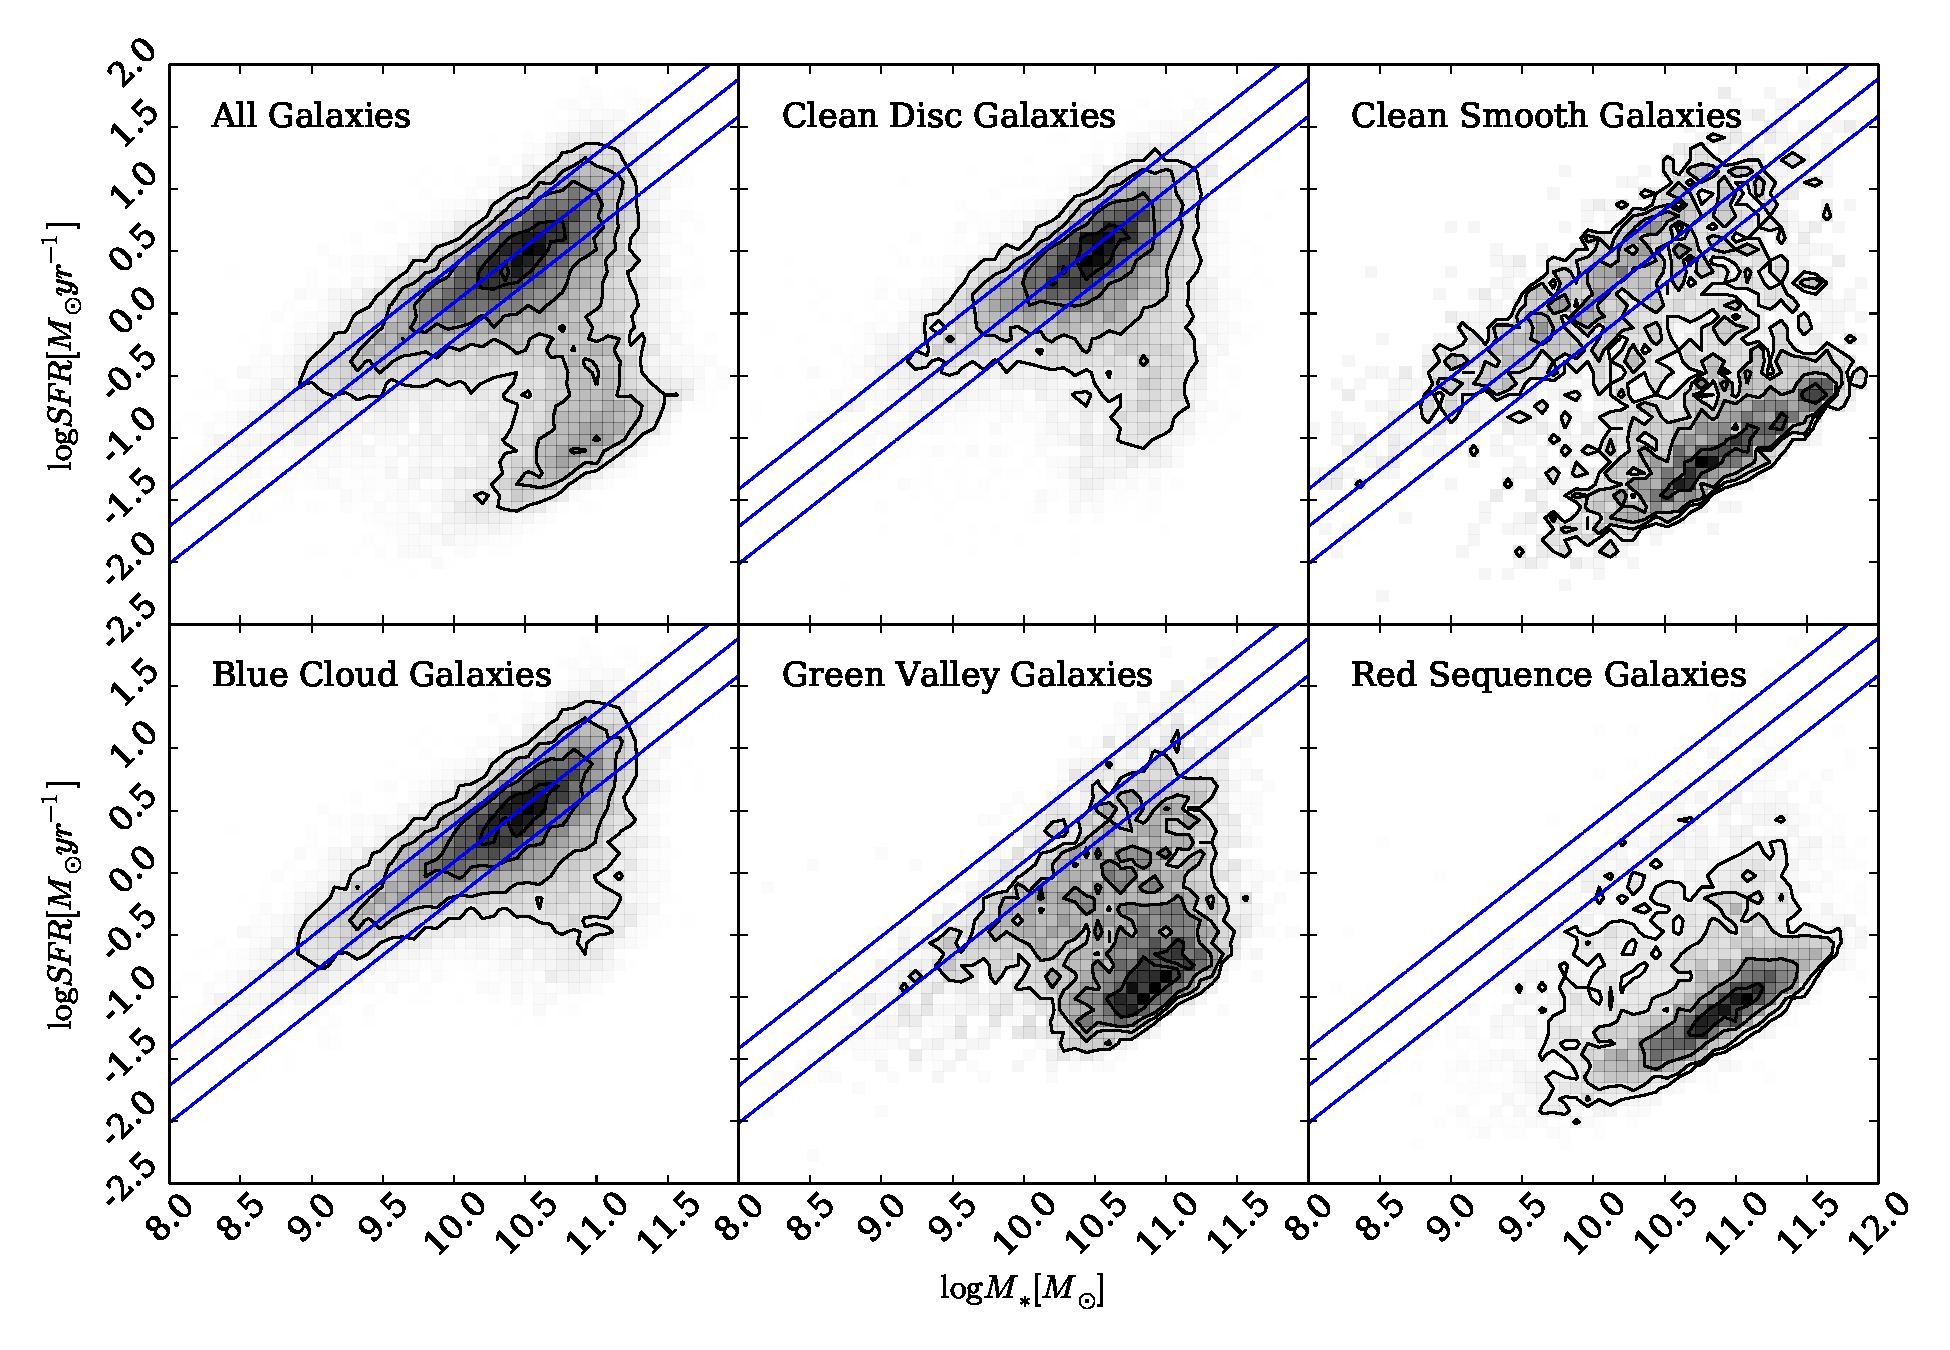
\includegraphics[width=0.9\textwidth]{sfr_mass_subsets.pdf}}
\caption{Star formation rate versus stellar mass diagrams show how the different populations of galaxies contribute to the `main sequence' (from \citet{Peng}, shown by the solid blue line with 0.3 dex scatter by the dashed lines) of star formation for the Galaxy Zoo 2 sample. This shows why the green valley is considered a transitional population between the blue cloud and the red sequence in terms of star formation rate. Interestingly, when we compare those galaxies which reside on the main sequence we find that the tail ends of this population (the low and high mass galaxies) are primarily made up of smooth (i.e. elliptical) galaxies as opposed to disc galaxies. The clean smooth and disc samples are described in \ref{class}.}
\label{sfr_mass_sub}
\end{figure*}

The intermediate green colours of these galaxies have been interpreted as evidence for recent quenching (suppression) of star formation \citep{Salim07}. Quenching causes a galaxy to leave the so-called `main sequence' of star formation \citep{Noeske07, Peng}, as shown in figure \ref{sfr_mass_sub} by the solid blue line (with $\pm ~0.3$ dex scatter shown by the dashed lines). Those galaxies whose star formation has ceased are found below the `main sequence'. The processes which cause these galaxies to depart from this sequence however, are still unknown \citep{Salim07, Peng, Elbaz11, Lee12} .

By studying the galaxies which  have just left this `main sequence' we can probe the quenching mechanisms by which this occurs. We can see from the lower panels of figure \ref{sfr_mass_sub}, which have split our sample into blue cloud, green valley and red sequence galaxies (see section \ref{defGV}), that the green valley galaxies are indeed a population which have either, left, begun to leave the `main sequence' or have some recent star formation. They are therefore an ideal population to probe the mechanisms behind this `crossroads` of galaxy evolution.


There have been many previous theories for the initial triggers of these quenching mechanisms, including negative feedback from AGN \citep{Sch07}, mergers \citep{Darg}, supernovae winds \citep{MFB12} and secular evolution \citep{Masters10, Masters11}. By investigating the \emph{amount} of quenching that has occurred between the blue cloud, green valley and red sequence (the three populations) we can apply a constraint to these mechanisms in order to decipher which, if any, are most dominant. 

We have been motivated by (i) \citet{Peng} who showed there may be at least two different quenching processes causing a migration from the `main sequence', (ii) \citet{Martin07} who used spectroscopic features to obtain information of the star formation histories of green valley galaxies to measure the mass flux across it and (iii) a previous Galaxy Zoo investigation by  \cite{Sch2014}, who by using a toy model found two contrastingly different evolutionary pathways between morphological types across the green valley. Unlike these previous studies this investigation utilises Bayesian statistics (for a comprehensive overview of Bayesian statistics see either \citealt{MacKay} or \citealt{Sivia}) in order to find the most likely toy model description of the star formation histories of galaxies in the three populations. It also provides a direct comparison with our current understanding of galaxy evolution from stellar population synthesis (SPS, see section \ref{SPS}) models. 

\section{Data}\label{data}
\subsection{Multi-wavelength data}\label{multi}
\begin{table*}
\begin{tabular*}{0.9\textwidth}{r| @{\extracolsep{\fill}}cccc}
\hline
\begin{tabular}[c]{@{}c@{}} {\color{white} -} \\ {\color{white} -}  \end{tabular} & All                                                      & Red Sequence                                              & Green Valley                                              & Blue Cloud \\  \hline 
Smooth ($p_s > 0.5$)        & \begin{tabular}[c]{@{}c@{}}42453\\ (33.6\%)\end{tabular} & \begin{tabular}[c]{@{}c@{}}17424\\ (13.8\%)\end{tabular}  & \begin{tabular}[c]{@{}c@{}}10687\\ (8.4\%)\end{tabular}   & \begin{tabular}[c]{@{}c@{}}14342\\ (11.3\%)\end{tabular}  \\ 
Disc ($p_d > 0.5$)          & \begin{tabular}[c]{@{}c@{}}83863\\ (66.4\%)\end{tabular} & \begin{tabular}[c]{@{}c@{}}10722\\ (8.4\%)\end{tabular}   & \begin{tabular}[c]{@{}c@{}}13257\\ (10.5\%)\end{tabular}  & \begin{tabular}[c]{@{}c@{}}59884\\ (47.4\%)\end{tabular}  \\
Early-type ($p_s \geq 0.8$) & \begin{tabular}[c]{@{}c@{}}10517\\ (8.3\%)\end{tabular}  & \begin{tabular}[c]{@{}c@{}}5337\\ (4.2\%)\end{tabular}    & \begin{tabular}[c]{@{}c@{}}2496\\ (2.0\%)\end{tabular}    & \begin{tabular}[c]{@{}c@{}}2684\\ (2.1\%)\end{tabular}    \\
Late-type ($p_s \geq 0.8$)  & \begin{tabular}[c]{@{}c@{}}51470\\ (40.9\%)\end{tabular} & \begin{tabular}[c]{@{}c@{}}4493\\ (3.6\%)\end{tabular}    & \begin{tabular}[c]{@{}c@{}}6817\\ (5.4\%)\end{tabular}    & \begin{tabular}[c]{@{}c@{}}40430\\ (32.0\%)\end{tabular}  \\ \hline
\textbf{Total}                       & \begin{tabular}[c]{@{}c@{}}\textbf{126316} \\ (100.0\%)\end{tabular}                                                & \begin{tabular}[c]{@{}c@{}}28146 \\ (22.3\%)\end{tabular} & \begin{tabular}[c]{@{}c@{}}23944 \\ (18.9\%)\end{tabular} & \begin{tabular}[c]{@{}c@{}}74226 \\ (58.7\%)\end{tabular} \\\hline
\end{tabular*}
\caption{Table showing the break down of the GZ2 sample into the subsets of the colour-magnitude diagram by galaxy type.}
\label{subs}
\end{table*}

Through this novel approach, we aim to determine the following:
\begin{enumerate}
\item What previous star formation history (SFH) causes a galaxy to reside in the green valley at the current epoch?
\item Why is the green valley so sparsely populated?
\item Is the green valley a transitional or static population? 
\item If the green valley is a transitional population then how many routes through it are there? 
\item Are there morphological dependant differences between these routes through the green valley? 
\end{enumerate}

This paper proceeds as follows. Section \ref{data} contains a description of the sample data, which is used in the Bayesian analysis of an exponentially declining star formation history model, all described in section \ref{models}. Section \ref{results} contains the results produced by this analysis, with section \ref{diss} providing a detailing discussion of the results obtained. We also conclude our findings in section \ref{conc}. The zero points of all ugriz magnitudes are in the AB system and where necessary we adopt the WMAP Seven-Year Cosmological parameters \citep{WMAP} with $(\Omega_m, \Omega_{\lambda}, h) = (0.26, 0.73, 0.71)$. 


In this section we will describe the data used in this paper. The galaxy sample is compiled from publicly available data from the Sloan Digitial Sky Survey (SDSS; \citealt{York00}) Data Release 8 \citep{Aihara11}. Optical photometry was obtained from this survey using the CAS-JOBS service on behalf of the Virtual Observatory (VO). Near-ultraviolet (NUV) photometry was obtained from the Galaxy Evolution Explorer (GALEX; \citealt{Martin05}) and was matched using the VO (via TOPCAT; \citealt{Taylor05}) with a search radius of $1''$ in right ascension and declination. 

Observed optical and ultraviolet fluxes are corrected for dust reddening using estimates from \citet{Oh11} of internal extinction by applying the \citet{Cardelli89} law. We also adopt k-corrections $z=0.0$ from the NYU-VAGC \citep{Blanton05, Pad08, BR07} with a typical $u-r$ correction of $\sim 0.05$ mag. Omitting these corrections does not change the results significantly. 

We obtained star formation rates (corrected for aperture and extinction) and stellar masses from the MPA-JHU catalog \citep{Kauff03, Brinch04}, which are in turn calculated from the SDSS spectra and photometry. 

\begin{figure}
\centering{
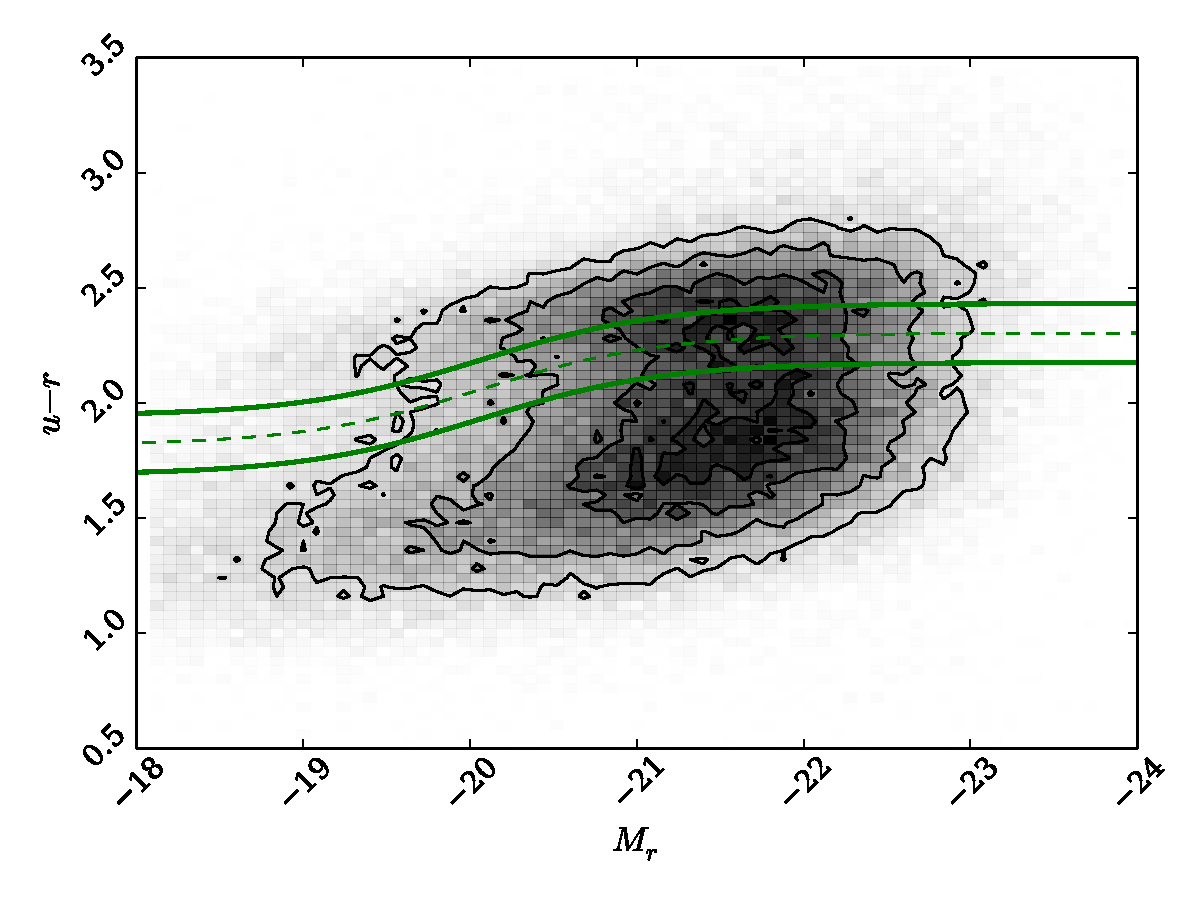
\includegraphics[width=0.45\textwidth]{col_mag_with_GV.pdf}}
\caption{Colour-magnitude diagram for the Galaxy Zoo 2 population showing the definition between the blue cloud and the red sequence from \citet{Baldry04} with the dashed line. The solid lines show $\pm 1\sigma$ either side of this definition; any galaxy within the boundary of these two solid lines is considered a green valley galaxy.}
\label{CMGV}
\end{figure}

\subsection{Galaxy Zoo 2 Morphological classifications}\label{class}

\begin{figure*}
\centering{
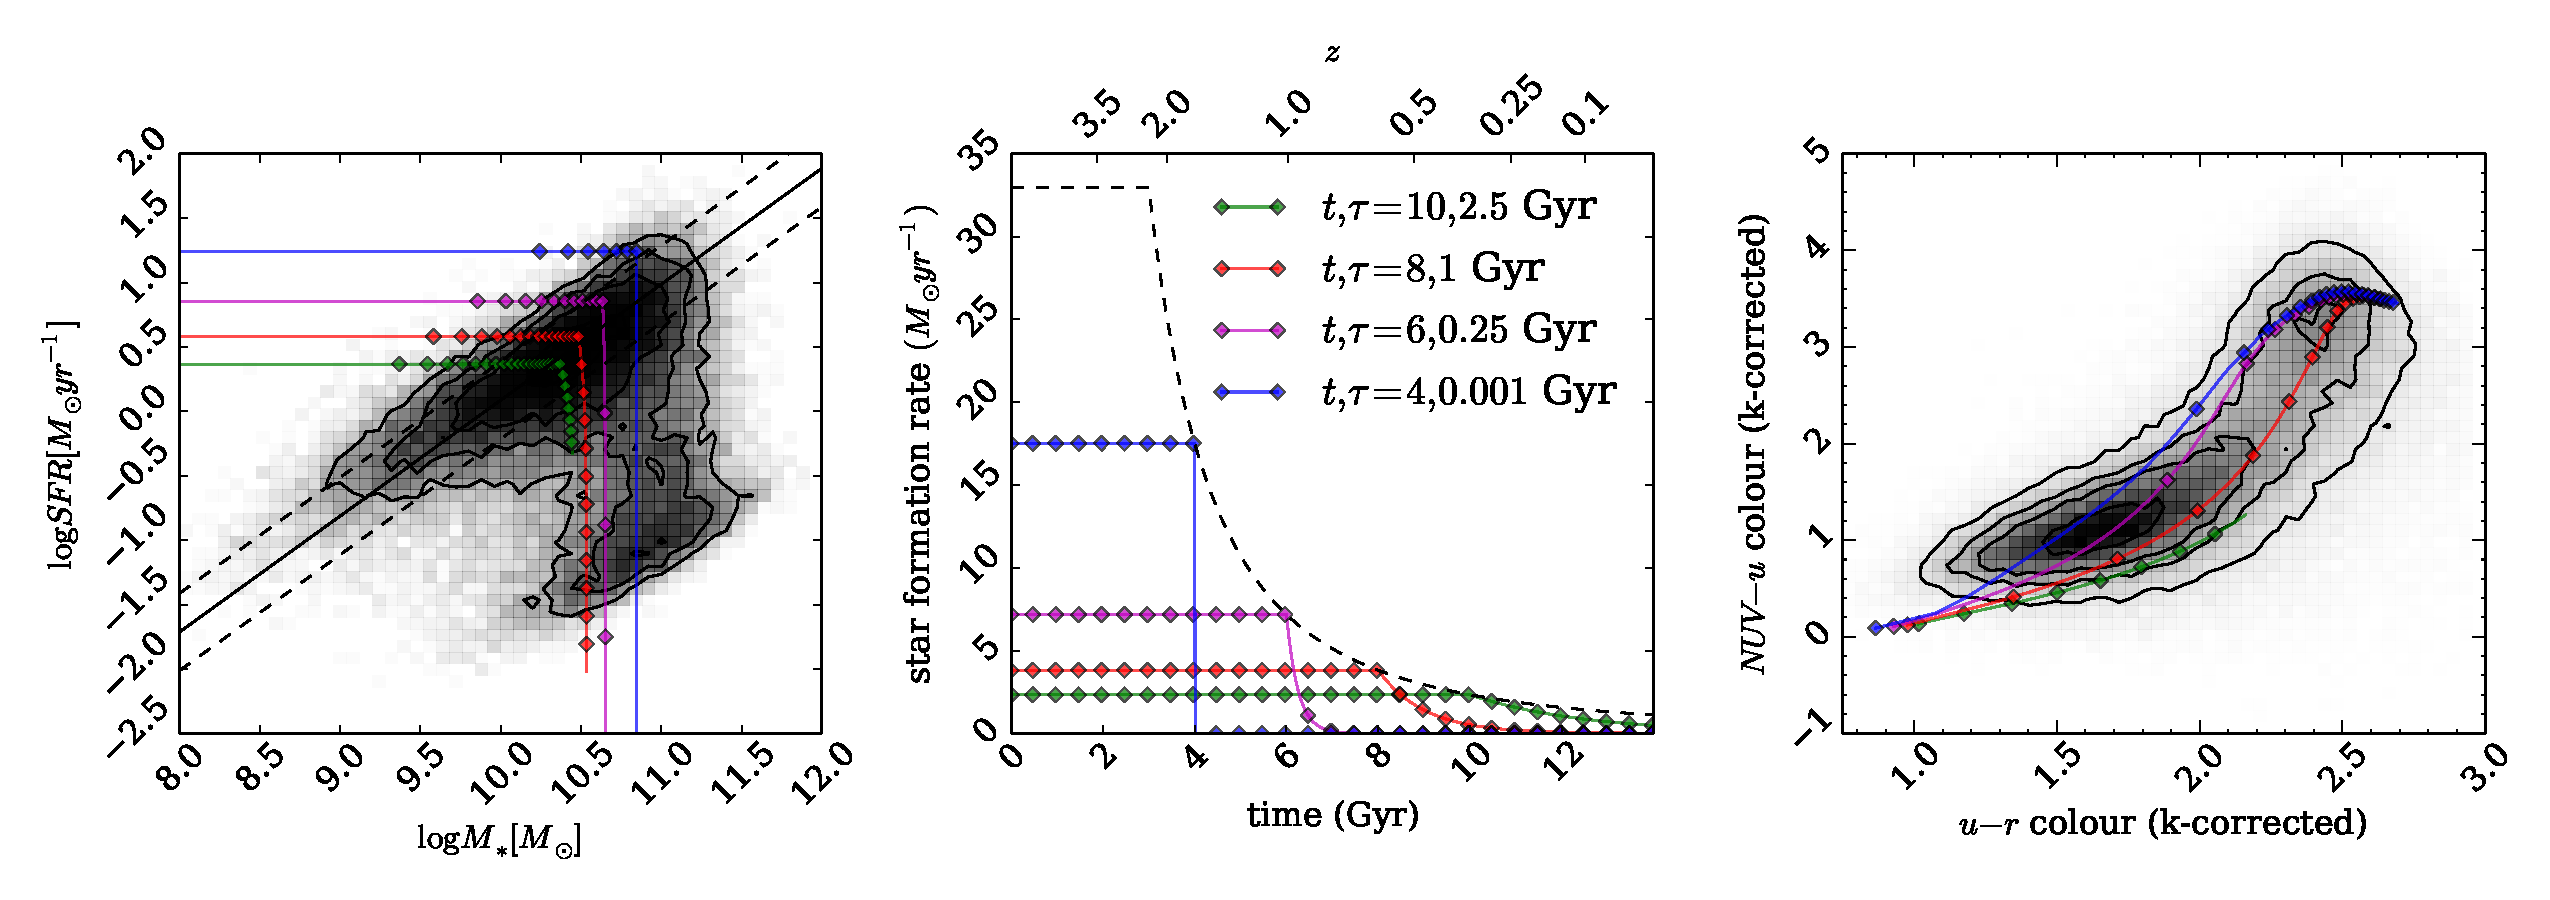
\includegraphics[width=\textwidth]{sfr_mass_colour_diagram.pdf}}
\caption{The SFR versus time for four model galaxies with various star formation histories are shown in the middle panel of this diagram.The dashed line shows the relationship between the sSFR and time from \citet{Peng} which was used to constrain these models at $t=t_{quench}$. The evolution of each of these four model galaxies across the SFR-mass diagram (from $t=0~Gyr$) and optical-NUV colour-colour diagram (from $t=t_q$) are shown in the left and right panels respectively; with each point representing a time step of $t=0.5~Gyr$. These plots show how the models are capable of reproducing the observed properties of the GZ2 sample of galaxies.}
\label{sfr_mass_col}
\end{figure*}

In this investigation we utilise visual classifications of galaxy morphologies from the Galaxy Zoo 2\footnote{\url{http://zoo2.galaxyzoo.org/}} citizen science project \citep{GZ2}. The project is able to provide these morphologies by obtaining multiple independent classifications for each galaxy image. Since it's inception in 2007, more than 1,000,000 SDSS and Hubble galaxy images have been classified by $\sim 40$ independent volunteers each, via a website. The initial version of the project, Galaxy Zoo 1 \citep{Lintott09, Lintott11}, asked a single question for each image (whether the galaxy was spiral or elliptical), however subsequent versions\footnote{\url{http://www.galaxyzoo.org/}} have collected more detailed information about each galaxy's morphology; such as bulge strength, bars and the presence of mergers (for detailed analysis of the classifications from questions such as these see: \citealt{Darg, Sch09, Masters11, Masters12, Simmons13, Cheung13, Melvin14})

This work uses classifications collected during the second release of the project; Galaxy Zoo 2 \citep{GZ2}, for which the full question tree for each image is shown in figure 1 of \citet{GZ2}. The first question posed by the study again asks volunteers to chose whether a galaxy is mostly smooth, is featured or is a star/artifact. Unlike other questions further down in the decision tree, every user who classifies a galaxy image will respond to this question (others, such as whether the galaxy has a bar, is dependant on a user having first classified it as a featured galaxy, therefore the number of classifications for that question depends on the previous responses of a user) therefore we have very statistically robust classifications at this level. 

The classifications from users produce a vote fraction for each galaxy; for example if 80 of 100 people thought a galaxy was disc shaped, whereas 20 out of 100 people thought the same galaxy was smooth in shape (i.e. elliptical), that galaxy would have vote fractions $p_{s} = 0.2$ and $p_{d} = 0.8$. In this example this galaxy would be included in the \emph{`clean'} disc sample ($p_d \geq 0.8$) according to \cite{GZ2} and would be considered a late-type galaxy. These vote fractions allow each galaxy to be considered in a large statistical analysis of how smooth and disc galaxies differ in their SFHs; the like of which has not been possible prior to this investigation and the Galaxy Zoo project. 




Specifically, the Galaxy Zoo 2 project consists of $304, 022$ images from the SDSS DR8 (a subset of those classified in Galaxy Zoo 1) all classified by \emph{at least} 17 independent users, with the mean number of classifications standing at $\sim42$. The only further selection that was made to the sample was for the removal of  objects considered to be stars or artifacts by the volunteers. Further to this, we required NUV photometry from the GALEX survey, within which $\sim42\%$ of the GZ2 sample were observed, giving a total sample size of $126316$ galaxies. 



\subsection{Definining the Green Valley}\label{defGV}


To define which of our sample of $126316$ galaxies were in the green valley, we used the definition outlined in \citet{Baldry04}, which is shown in figure \ref{CMGV} by the dashed line. Any galaxy within $\pm 1\sigma$ of this relationship, shown by the solid lines in figure \ref{CMGV}, was considered a green valley galaxy. A conservative definition for the green valley was adopted in order to remove any influence from tail galaxies from either the red sequence or blue cloud. The break down of our sample into red sequence, green valley and blue cloud galaxies is shown in table \ref{subs} along with a further break down by galaxy type. 


\section{A Bayesian Analysis}\label{models}
\subsection{Stellar Population Synthesis Models}\label{SPS}
The observed features of galactic spectra can be modelled using simple stellar population techniques which sum the contributions of individual stars to the spectra, assuming that these stars are coeval and form with the same metallicity. The accuracy of these predictions therefore depends on the stellar completeness of the input physics. Comprehensive knowledge is therefore required of (i) stellar evolutionary tracks and (ii) the initial mass function (IMF) to synthesise a stellar population accurately. These stellar population synthesis (SPS) models are an extremely well debated area of astrophysics \citep{Maraston06, Eminian08, CGW09, Falk09, Chen10, Kreik10, MRC11, Mel12}. In this investigation we utilised the \citet{BC03} \emph{GALEXEV} SPS models along with a Chabrier (ref) IMF, across a large wavelength range ($91 \AA < \lambda < 160 \mu m$), at solar metalicity (m62 in the \citet{BC03} models), across cosmic time. 

\subsection{Star Formation Histories}\label{sfh}
\begin{figure*}
\centering{
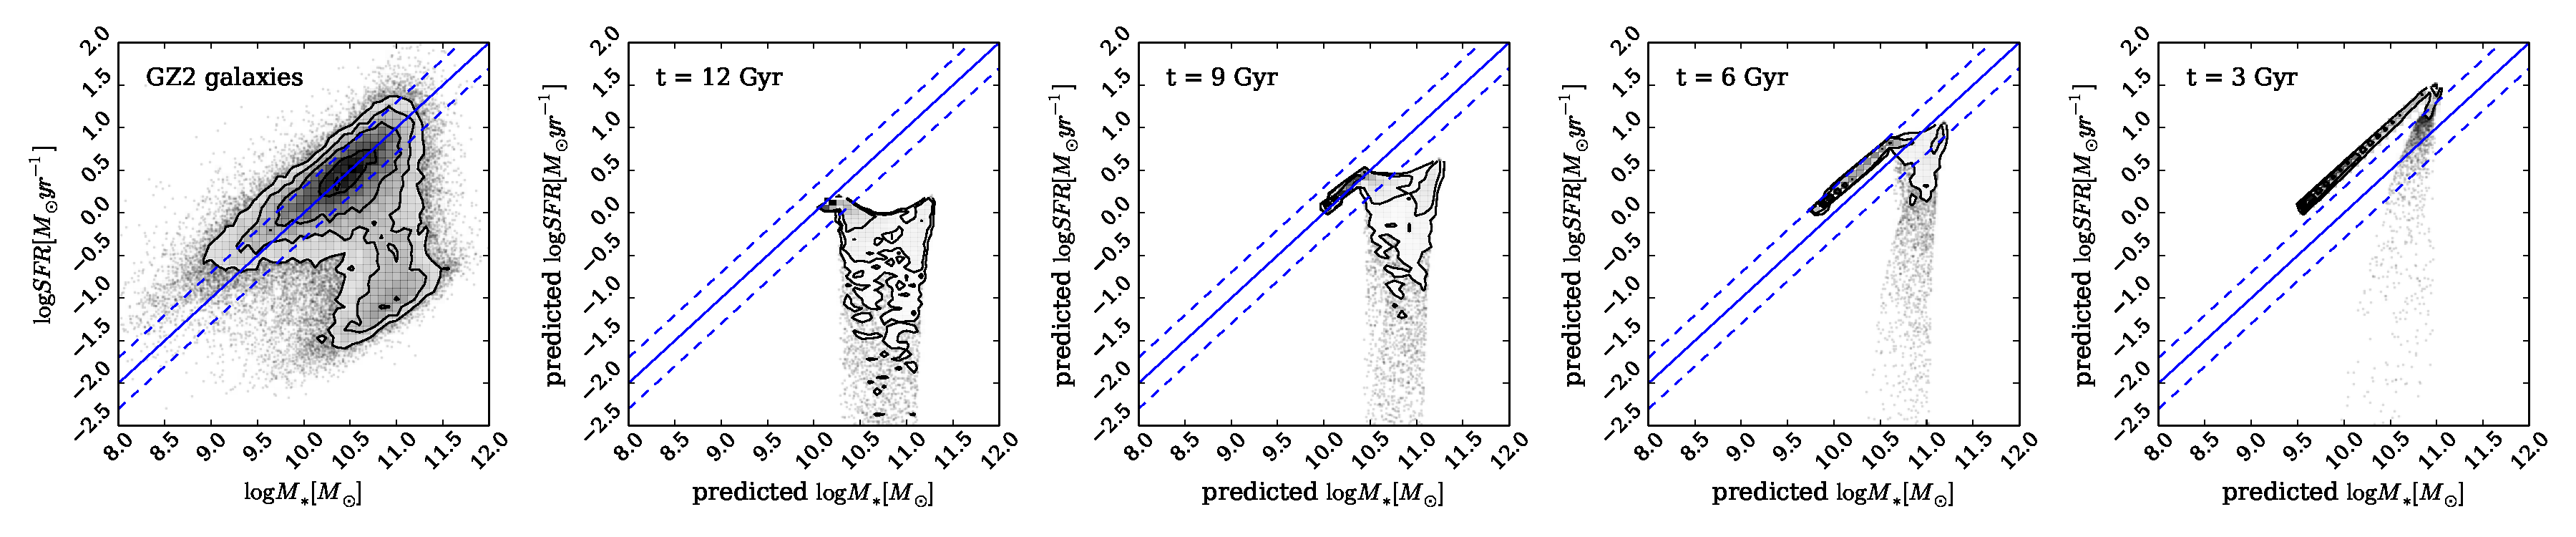
\includegraphics[width=\textwidth]{sfr_mass_evo.pdf}}
\caption{Plots to show the evolution of the SFR against the mass as predicted by the most likely exponential SFH model for each GZ2 galaxy. Each panel shows the models at different look-back times in the history of the Universe. The panel on the far left also includes the contours of the observed SFR against the mass of the GZ2 galaxies. Each panel also shows the `main sequence' of star formation from \citet{Peng} for a galaxy of mass $M=10^{10.27} M_{\odot}$ at the various epochs; hence the apparent deviation from the model `main sequence' with cosmic time.}
\label{sfr_mass_evo}
\end{figure*}

In our model we assume the following:
\begin{enumerate}
\item galaxies evolve only from blue to red colours
\item all galaxies formed at a time t=0 with an initial burst of star formation 
\item the star formation history (SFH) of a galaxy can be modelled as an exponentially declining star formation rate (SFR) across cosmic time ($0 \leq t [Gyr] \leq 13.8$) as:

\[
SFR = 
\begin{cases}
c_{SFR} & \text{if } t < t_{q} \\
c_{SFR} \times exp{\left( \frac{-(t-t_{q})}{\tau}\right)} & \text{if } t > t_{q}
\end{cases}
\]
\end{enumerate}
where $t_{q}$ is the onset time of quenching, $\tau$ is the timescale over which the quenching occurs and $c_{SFR}$ is a constant star formation rate. This constant star formation rate is set using \citet{Peng}, who defined a relation (in their equation 1) between the average SFR and cosmic time as:
\begin{equation*}
sSFR(m,t) = 2.5 \left( \frac{m}{10^{10} M_{\odot}} \right)^{-0.1} \left(\frac{t}{3.5}\right)^{-2.2} Gyr^{-1}
\end{equation*}



At the point of quenching, $t_{q}$, the models are defined to have a SFR which lies on this relationship for a galaxy with mass, $M = 10^{10.27} M_{\odot}$, the average mass of the GZ2 sample; see figure \ref{sfr_mass_col}. \citet{Peng} state that beyond $z \sim 2$ the characteristic SFR flattens and is roughly constant back to $z\sim6$. The cause for this change is not well understood but can be seen across similar observational data (\cite{Gonzalez} and \cite{Beth}). Motivated by these observations, we took the relation as defined in \citet{Peng} up to a cosmic time of $t=3~Gyr (z \sim 2.3)$ and prior to this assumed a constant average SFR, as shown by the dotted line in the middle panel of figure \ref{sfr_mass_col}.
 
We are aware that the average SFR of our models will result in a lower value than the relation defined in \citet{Peng} at all cosmic times with this treatment; each galaxy only resides on the `main sequence' at the point of quenching. However, as \citet{Beth} and \citet{Heinis14} point out, galaxies cannot remain on the `main sequence' from early to late times throughout their entire lifetimes given the resultant stellar masses and SFR this would infer at the current epoch in the local Universe. If we were to include prescriptions for no quenching, starbursts, mergers, AGN etc. into our models we would improve on our reproduction of the average SFR across cosmic time; however in the interest of Occam's razor \citep{Sivia, Sok02} we decided to focus entirely on a quenching only model. 


The left panel in figure \ref{sfr_mass_col} shows how well these models reproduce the observed relationship between the SFR and the mass of a galaxy, including how at the time of quenching they reside on the \emph{`main sequence'} of star formation, shown by the solid black line for a galaxy of mass, $M = 10^{10.27} M_{\odot}$.  We can also see in figure \ref{sfr_mass_evo} how this diagram evolves with cosmic time according to our model predictions. 



In our models a smaller $\tau$ value corresponds to a rapid quench (almost instantaneous suppression of star formation), whereas a large value of $\tau$ corresponds to a slower quench (slower than the dynamical timescale of a galaxy).  This model assumes that all of the populations form an initial burst of stars at $t=0$, the mass of which is set by the value of $c_{SFR}$. %The $c_{SFR}$ value is set by using the relation defined in \citet{Peng} between the average sSFR and the lookback time (i.e. redshift); at $t_{quench}$ the SFR is set to lie on this relationship (see bottom panel of figure \ref{kev}). 

Once this evolutionary SFR is obtained, we convolve it with the \citet{BC03} population synthesis models to generate a model SED at each time step. We suppress the fluxes from stars younger than $3~Myr$ to mimic the effect of birth clouds, then apply filter transmission curves to obtain AB magnitudes and therefore colours. How these colours evolve from the point of quenching onwards in the optical-NUV colour space can be seen in the right panel of figure~\ref{sfr_mass_col}.



Given that we have information about these modelled populations across all cosmic time, we can \emph{`observe'} these model stellar populations at a given time in their history; this correlates to the lookback time and therefore, if they were real populations, a measurable redshift (assuming all galaxies are formed at a time $t=0$). This lookback time $t^{lb}$ can be thought of as a galaxy's age, again if we assume that all galaxies formed with an initial burst of star formation at $t=0$. Therefore, for each galaxy in the GZ2 sample, the lookback time was calculated from the redshift (using the \emph{cosmolopy} package provided in the Python module \emph{astroPy}\footnote{\url{http://www.astropy.org/}}; \citealt{Rob13}) in order to compare the observed colours to the predicted models colours at that time. 

Figure \ref{pred} shows the predicted optical and NUV colours at a time of $t^{lb} = 12.8 ~Gyr$ (the average look back time of the Galaxy Zoo 2 sample, $z~0.076$) provided by the exponential SFH model. These predicted colours will be referred to as $d_{c,p}(t_{q}, \tau, t^{lb})$ (where c=\{opt,NUV\}). The SFR at a time of $t^{lb}=12.8~Gyr$ is also shown in Figure \ref{pred} to compare how this correlates with the predicted colours. The $u-r$ predicted colour shows an immediate correlation with the SFR, however the $NUV-u$ colour is more sensitive to the value of $\tau$ and so is ideal for tracing any recent star formation in a population . At small $\tau$ (rapid quenching timescales) the $NUV-u$ colour is insensitive to $t_{q}$, whereas at large $\tau$ (slow quenching timescales) the colour is very sensitive to $t_{q}$. Together the two colours are ideal for tracing the effects of $t_{q}$ and $\tau$ in a population. 


\begin{figure}
\centering{
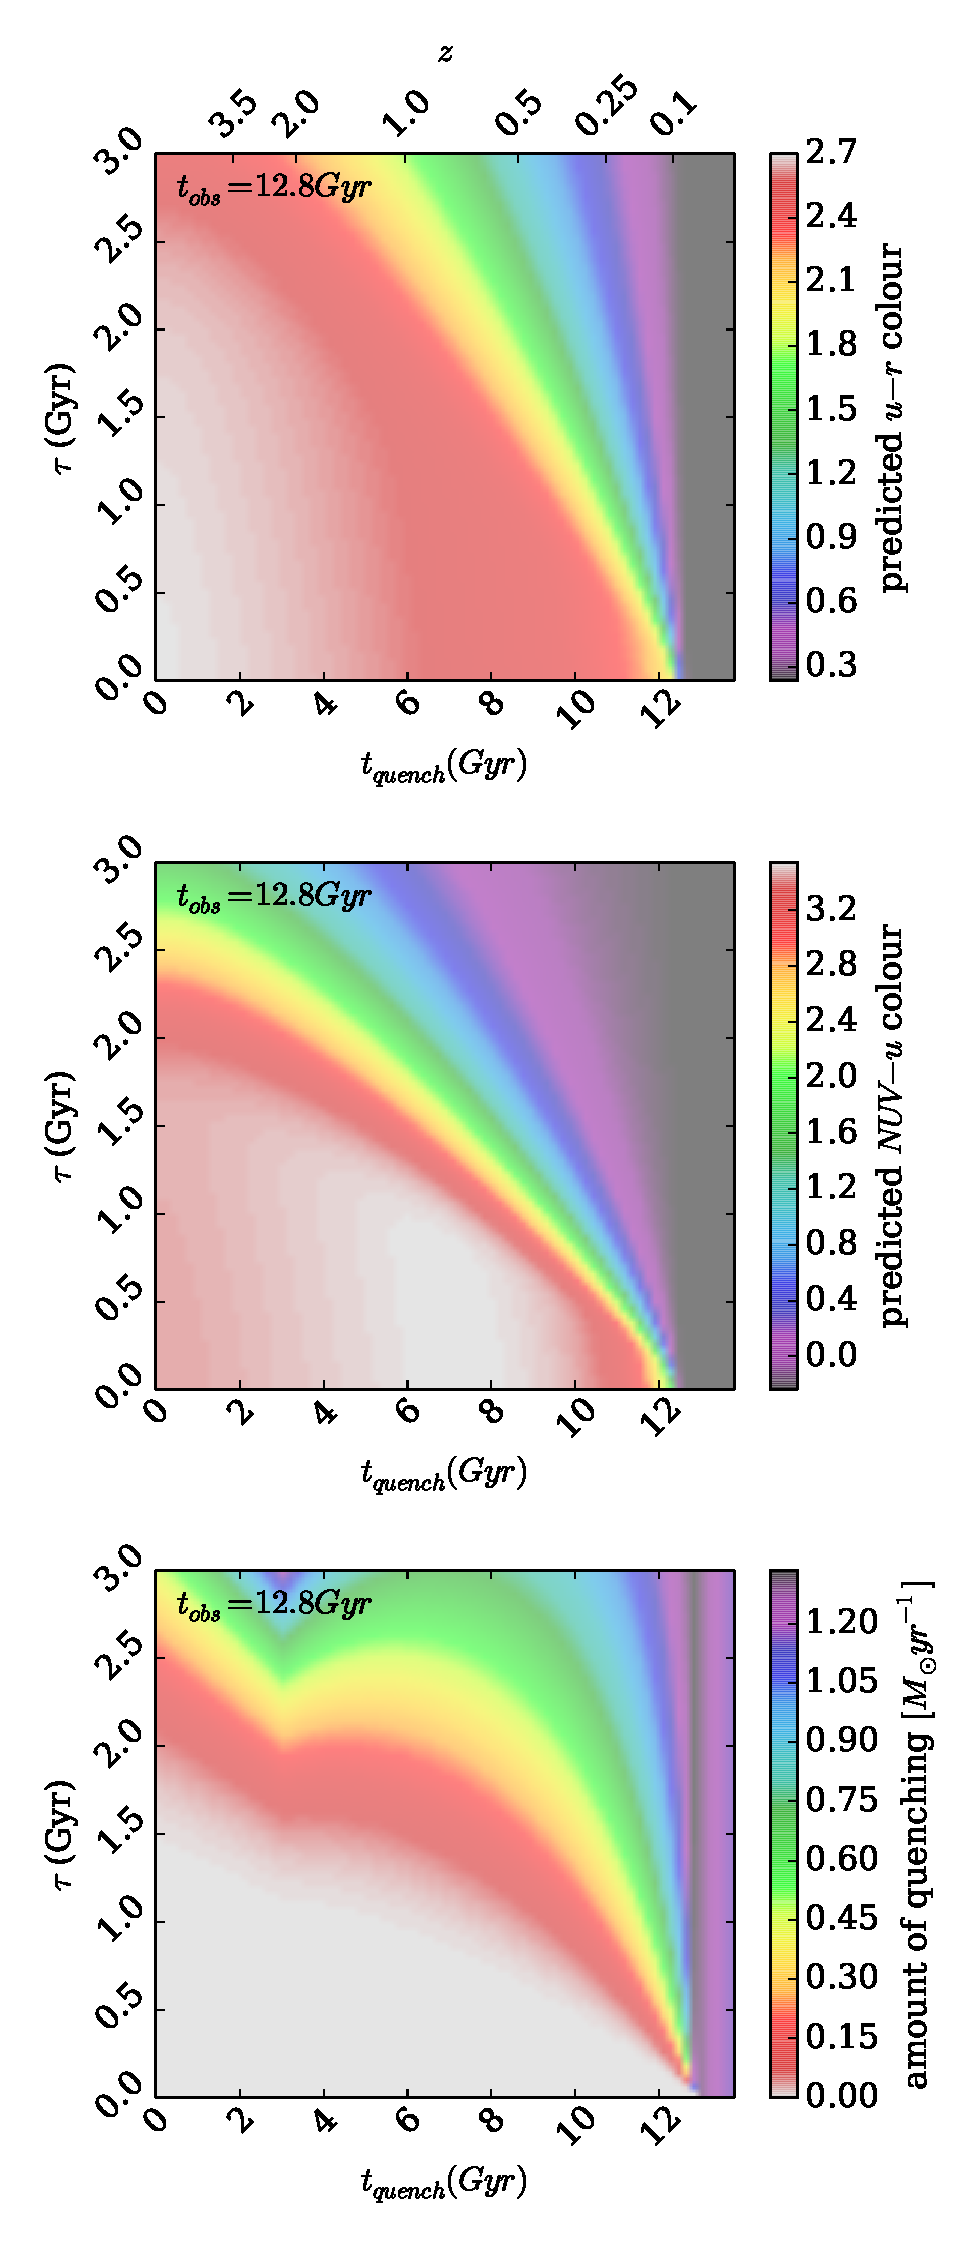
\includegraphics[width=0.45\textwidth]{colours.pdf}}
\caption{Model predictions of the $u-r$ and $NUV-u$ colours in the top and  middle panels respectively when the populations are observed at $t^{lb} = 12.8~Gyr$ (the average look back time of the GZ2 sample, calculated from the observed redshifts). In the bottom panel, the SFR at a time of $t^{lb} = 12.8 ~Gyr$ predicted by the models is shown. In all three plots, it can be seen that the models with $t_q > 12.8~Gyr$ have not undergone any quenching, as they have been `observed' before this time. They are therefore still star forming and show the bluest colours and highest SFRs.}
\label{pred}
\end{figure}


\subsection{Bayesian Analysis}\label{stats}
In order to achieve robust conclusions we conduct a a fully Bayesian analysis \citep{Sivia, MacKay} of our SFH models in comparison to the observed GZ2 sample data. To do this we must consider all possible combinations of $(t_{q}, \tau) = \theta$ which will be distributed with a mean, $\mu$ and standard deviation, $\sigma$, so that:
\begin{equation*}
w = (\mu_{\theta}, \sigma_{\theta}) = (\mu_{t_{q}}, \sigma_{t_{q}}, \mu_{\tau}, \sigma_{\tau})
\end{equation*}
We can then define a Bayesian probability for a combination of $\theta$ values \underline{given} what we know about $w$: $P(\theta|w) = P(t_{q}, \tau|w) = P(t_{q}|w)P(\tau|w)$ assuming that $ P(t_{q}|w)$ and $P(\tau|w)$ are independent of each other, so that:
\begin{multline*}
P(t_{q}, \tau|w) = \frac{1}{\sqrt[]{4\pi^2\sigma^2_{t_{q}}\sigma^2_{\tau}}} \exp\left[-\frac{(t_{q}-\mu_{t_{q}})^2}{2\sigma^2_{t_{q}}}\right] \\ \exp\left[-\frac{(\tau-\mu_{\tau})^2}{2\sigma^2_{\tau}}\right].
\end{multline*}
This is equivalent to:
\begin{equation*}
P(\theta|w) = \frac{1}{Z_{\theta}} \exp\left[-\frac{\chi_{\theta}^2}{2}\right].
\end{equation*}
Therefore if we work in logarithmic probabilities:
\begin{equation*}
\log[P(\theta|w)] = - \log(Z_{\theta}) - \frac{\chi_{\theta}^2}{2}.
\end{equation*}
We must also find the probability of all of the GZ2 data ($\underline{d}$) \underline{given} a SFH model, i.e. a single combination of $\theta$ values, $P(\underline{d}|\theta, t_{k}^{lb})$:
\begin{equation*}
P(\underline{d}|\theta, t_{k}^{lb}) = \prod_{k} P(d_{k}|\theta, t_{k}^{lb}),
\end{equation*}
where $d_{k}$ is a single data point of one galaxy. Assuming that all galaxies formed at $t=0~Gyr$ with an initial burst of star formation, we can assume that the `age' of each galaxy in the GZ2 sample is equivalent to it's look-back time, $t^{lb}_{k}$, which can be calculated from it's observed redshift (see section \ref{class}). We then use this  `age' to calculate the predicted model colours at this cosmic time for a given combination of $\theta$: $d_{c,p}(\theta, t^{lb}_{k})$ for both optical $(c=opt)$ and NUV $(c=NUV)$ colours. We can now directly compare our model colours with the observed GZ2 galaxy colours, so that for a single galaxy k with optical ($u-r$) colour, $d_{opt, k}$ and NUV ($NUV-u$) colour, $d_{NUV,k}$, the Bayesian probability $P(d_{k}|\theta, t^{lb}_{k})$:

%We calculate $P(d_{k}|\theta, t_{k}^{lb})$ using the predicted values for the optical ($c=opt$) and NUV ($c=NUV$) colours, $d_{c,p}(\theta, t_{k}^{lb})$, for a given combination of $\theta = (t_{q}, \tau)$ and a calculated galaxy age $t^{lb}$ (look back time, calculated from a galaxy's redshift, equivalent to the age of the galaxy assuming that all galaxies formed at $t=0~Gyr$):

\begin{multline*}
P(d_{k}|\theta, t^{lb}_{k}) = \frac{1}{\sqrt{2\pi\sigma_{opt, k}^2}}\frac{1}{\sqrt{2\pi\sigma_{NUV, k}^2}} \\ \exp{\left[ - \frac{(d_{opt, k} - d_{opt, p}(\theta, t_{k}^{lb}))^2}{\sigma_{opt, k}^2} \right]} \\ \exp{\left[ - \frac{(d_{NUV, k} - d_{NUV, p}(\theta, t_{k}^{lb}))^2}{\sigma_{NUV, k}^2} \right]},
\end{multline*}
where for one combination of $\theta$,
\begin{equation*}
\chi_{c, k}^2 = \frac{(d_{c, k} - d_{c, p}(\theta, t_{k}^{lb}))^2}{\sigma_{c, k}^2}
\end{equation*}
and
\begin{equation*}
Z_{k} = \sqrt[]{2\pi\sigma_{c, k}^2}.
\end{equation*}
Again working in logarithmic probabilities:
\begin{equation*}
\log{(P(d_{k}|\theta, t^{lb}_{k}))} = \sum_{c} - \log{Z_{c,k}} - \sum_{c} \frac{\chi_{c, k}^2}{2}.
\end{equation*}
So that for all of the GZ2 galaxies:
\begin{equation*}
\log{(P(\underline{d}|\theta, \underline{t}^{lb}))} = \sum_{c, k} \log{(P(d_{c, k}|\theta, t_{k}^{lb}))}
\end{equation*}
\begin{equation*}
\log{(P(\underline{d}|\theta,  \underline{t}^{lb}))}  = K - \sum_{c, k} \frac{\chi_{c, k}^2}{2},
\end{equation*}
where K is a constant:
\begin{equation*}
K = - \sum_{c, k} \log{Z_{c, k}},
\end{equation*}
where $c=\{opt, NUV\}$. 



This gives us the probability of the data \underline{given} a specific model, however what we need is the probability of each combination of $\theta$ values \underline{given} the GZ2 data: $P(\theta|\underline{d}, t^{lb}, w)$, i.e. how likely is a single SFH model given the observed colours of all of the GZ2 galaxies. We can find this by:
\begin{equation*}
P(\theta|\underline{d}, t^{lb}, w) = \frac{P(\underline{d}|\theta, \underline{t}^{lb})P(\theta | w)}{\int P(\underline{d}|\theta, \underline{t}^{lb})P(\theta | w) d\theta},
\end{equation*}
where,
\begin{equation*}
P(\underline{d}|\theta, \underline{t}^{lb})P(\theta | w) = \exp{\left[\log{[P(\underline{d}|\theta, \underline{t}^{lb})]} + \log{[P(\theta | w)]}\right]},
\end{equation*}
The denominator is a mere normalisation factor, therefore when we compare the likelihoods between two different SFH models, i.e. two different combinations of $\theta = (t_{q}, \tau)$ we need only compare the numerator and can also remain in logarithmic probability space. So, given the data from the GZ2 sample, we can calculate $\log[P(\theta|\underline{d}, \underline{t}^{lb}, w)]$ for all possible $\theta$ values and compare these to determine the most likely values for $\theta$ given the GZ2 data. In order to this robustly, we performed a Markov Chain Monte Carlo (MCMC; \citealt{MacKay, Dan, GW10}) sampling method to cycle through the defined parameter space using a Python implementation of an affine invariant ensemble sampler by \cite{Dan}; \emph{emcee}.

This method allows for a speedier exploration of the parameter space by avoiding those areas with low likelihood. A large number of `walkers' are started at an initial position where the likelihood is calculated, from there they individually `jump' to a new area of parameter space. If the likelihood in this new area is greater than the original position then the `walkers' retain this position. This new position then influences the direction of the  `jumps' of other walkers.  This is repeated for the defined number of steps until the `walkers' have found the regions of highest likelihood.

In addition to the colours, the GZ2 data is unique in that it provides information on a galaxy's morphology, therefore we utilise the user vote fractions, see section \ref{class}. Specifically we consider how smooth-like, $p_s$ or disc-like, $p_d$ a galaxy is considered by volunteers. If either of these fractions is over $80\%$ then the galaxy is considered to be in the `clean' smooth or disc sample according to \citet{GZ2}. 

If we ran the above sampling method on galaxies in either of the \emph{clean} samples, we would lose all the information about the intermediate galaxies and how these contribute to the likelihood of $P(\theta|\underline{d})$. It is the intermediate galaxies which are thought to be crucial to the morphological changes between early- and late-type galaxies; if this change is associated with the green valley in any way then these vote fractions are information we wish to keep in our analysis. 

\begin{figure*}
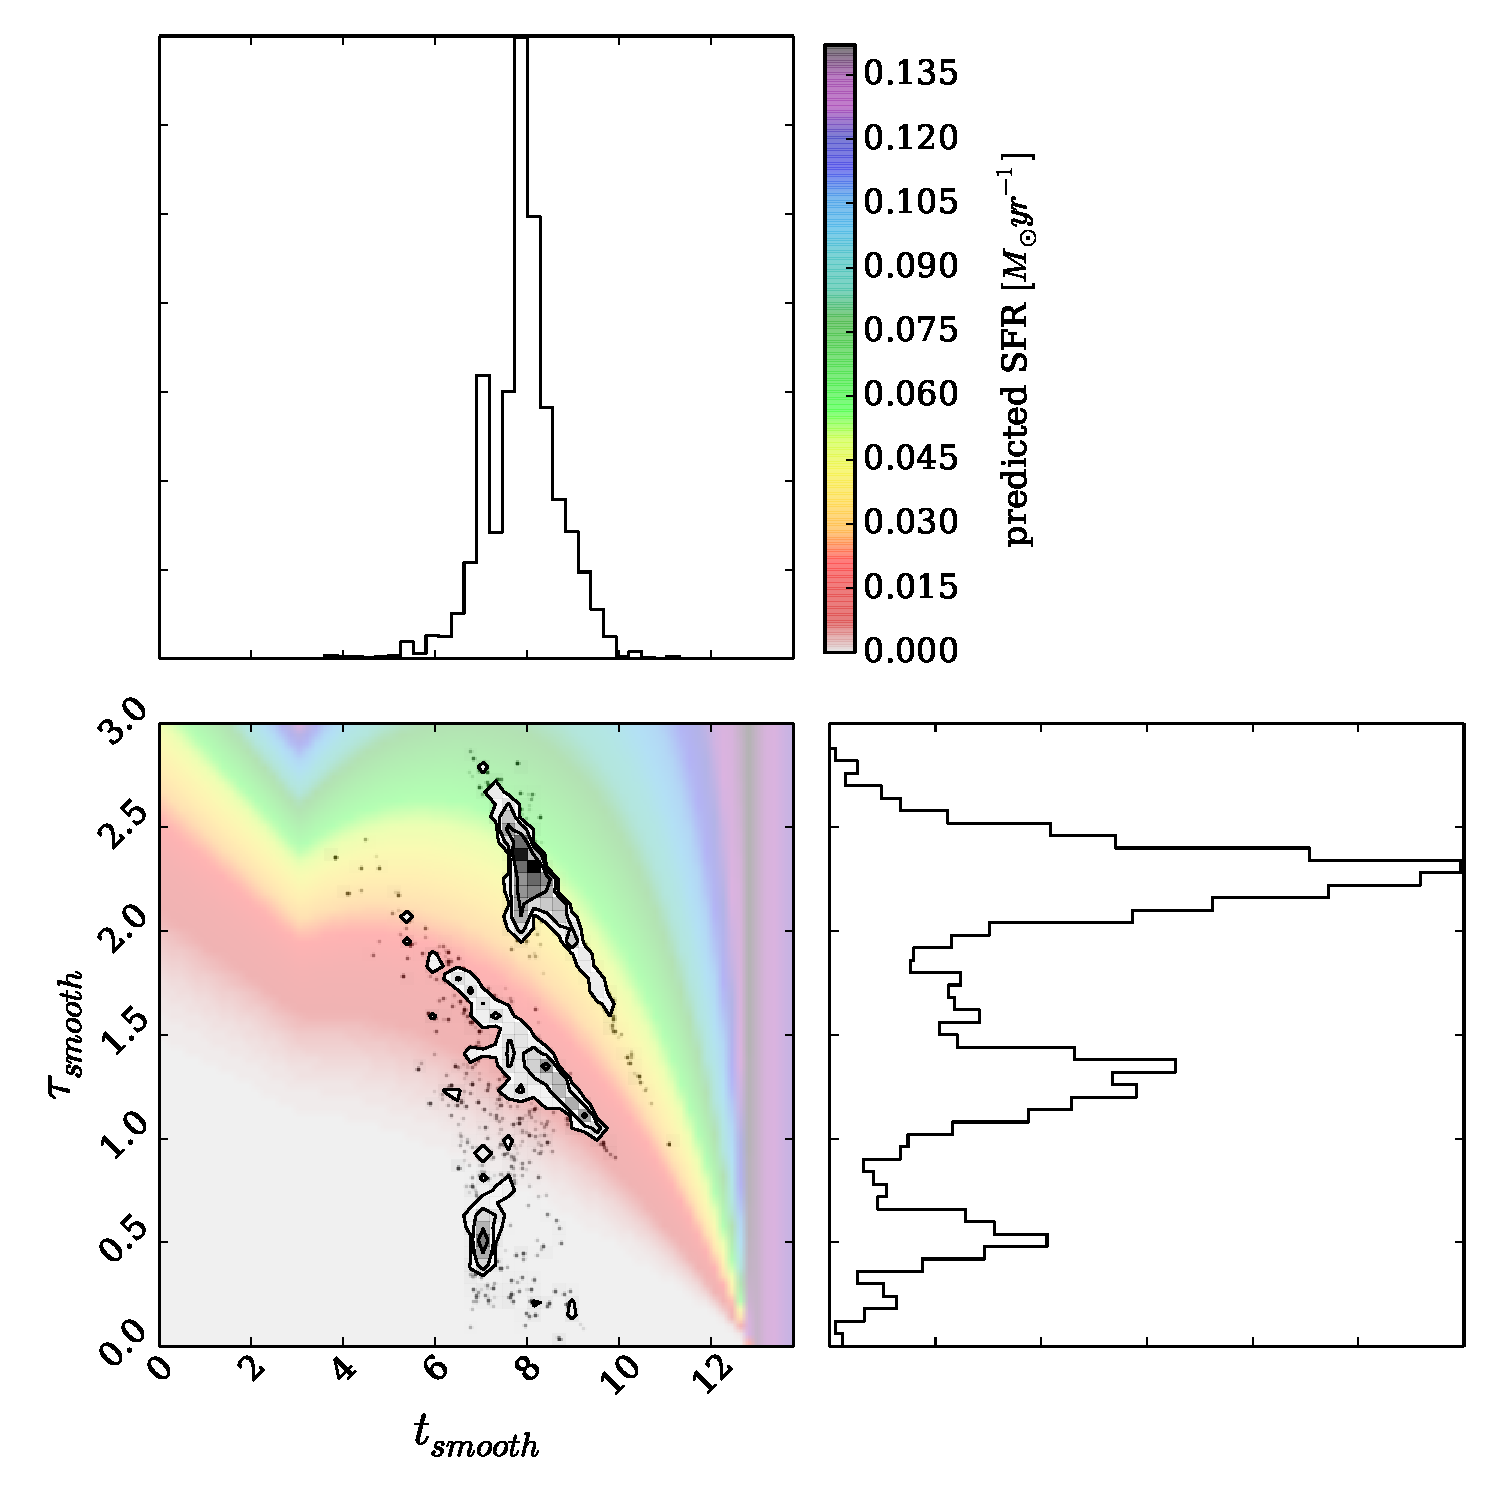
\includegraphics[width=0.4975\textwidth]{all_smooth.pdf}
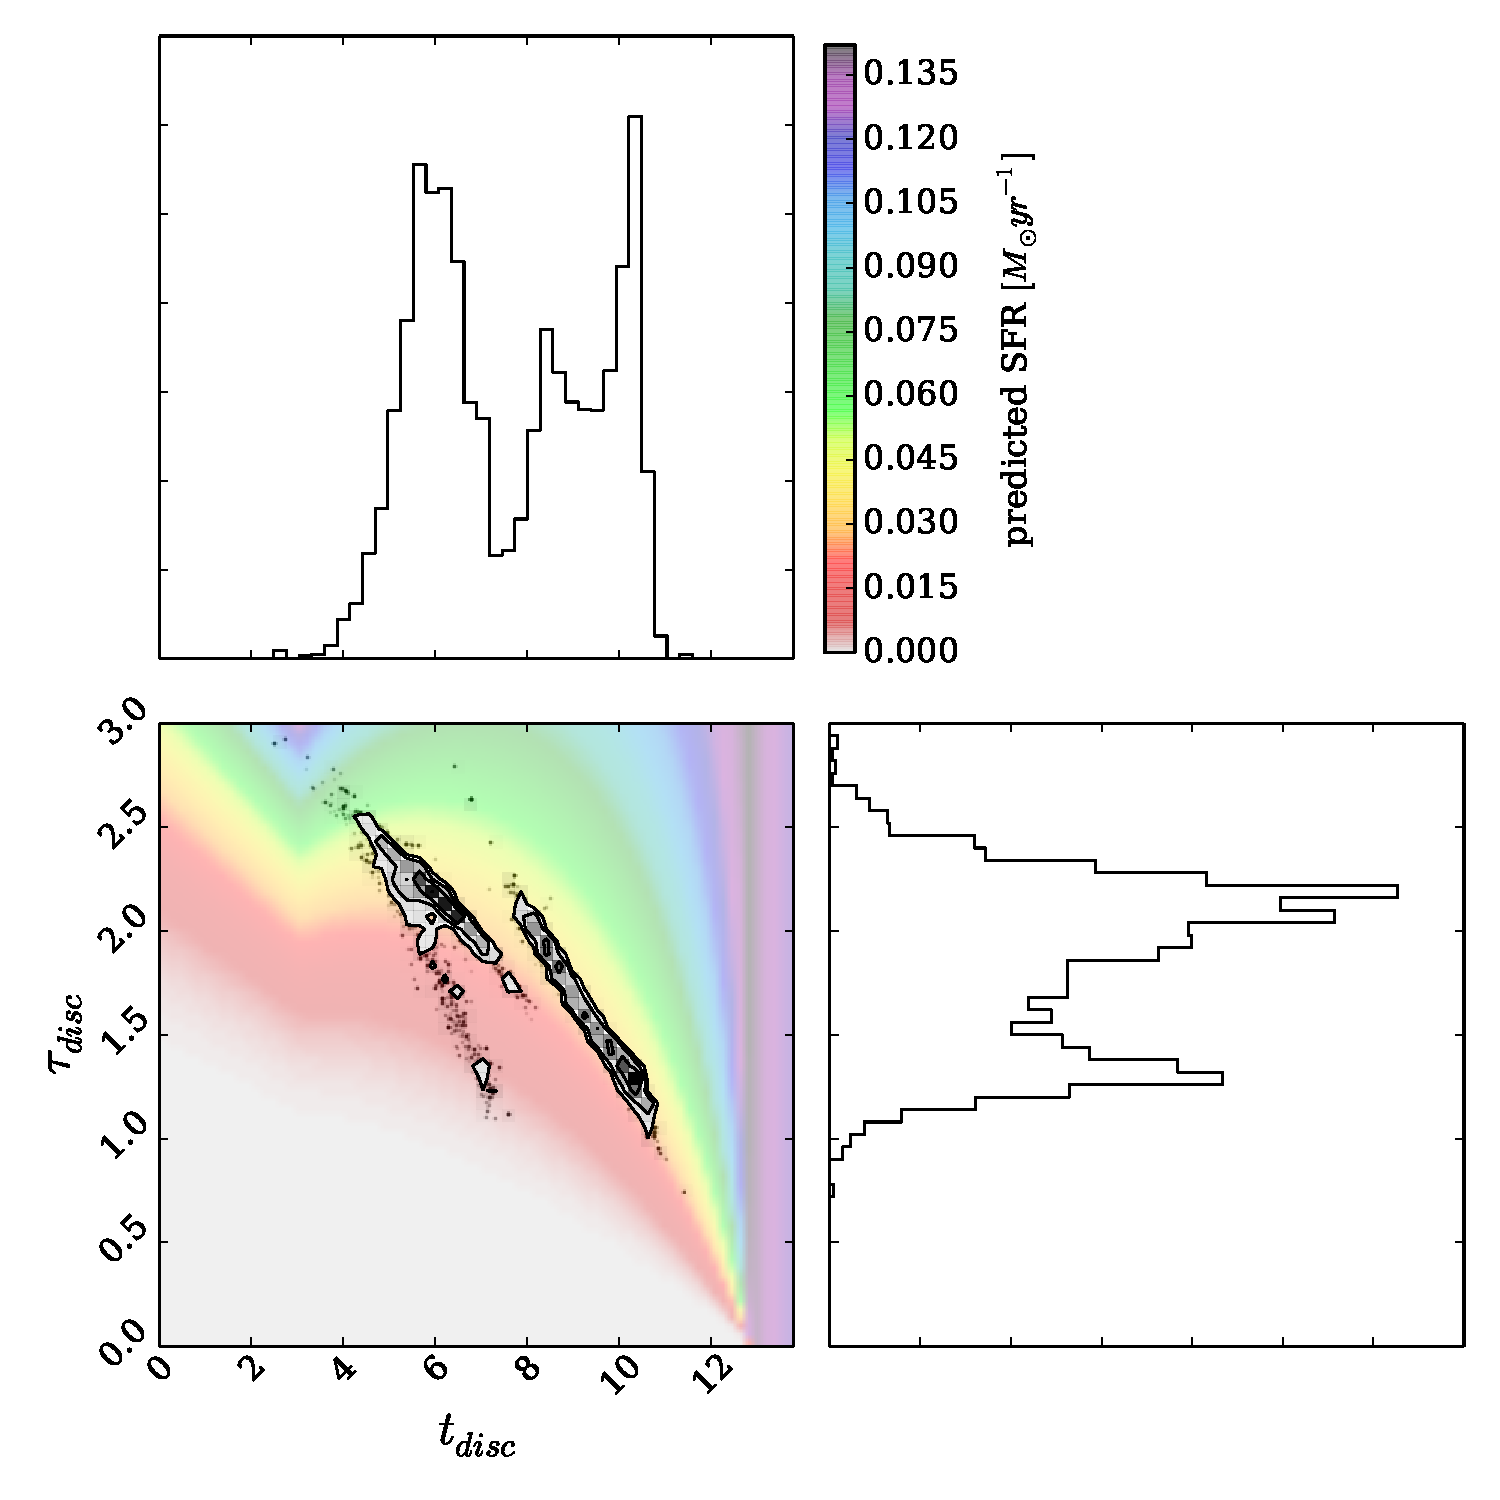
\includegraphics[width=0.4975\textwidth]{all_disc.pdf}
\caption[8pt]{For all the galaxies in the Galaxy Zoo 2 sample, contour and histogram plots show the regions of greatest likelihood for an exponential model star formation history parameters $[t_{quench}$ and $\tau_{quench}]$ for both smooth-like(left) and disc-like (right) galaxies. $t_{q}$ is the time at which quenching occurs (Gyr) and $\tau_{q}$ is the time scale on which quenching occurs (Gyr; the larger the $\tau_{q}$, the slower the quenching). Background colours show the star formation rate predicted by this model after a time $t \sim 12.8~Gyr$, which is the mean look back time of the galaxies in the GZ2 sample. Galaxies contribute  to $[t_{q}, \tau_{q}]_{smooth}$ and $[t_{q}, \tau_{q}]_{disc}$ according to their Galaxy Zoo 2 vote fraction (i.e. a galaxy with $p_{disc} \sim p_{smooth} \sim 0.5$ will contribute equally to each set of parameters).}
\label{all}
\end{figure*}

We incorporate these GZ2 vote fractions  into our sampling by considering them as weights to the likelihood $P(d_{k}|\theta, t^{lb}_{k})$ to which that galaxy contributes to $P(\underline{d}|\theta, \underline{t}^{lb})$. For example a galaxy which has $p_{s} = 0.9$ should carry more weight in the likelihoods for the model parameters to describe smooth galaxies than a galaxy with $p_{s} = 0.1$. Therefore the likelihood can now be thought of as:
\begin{equation*}
P(\underline{d}|\theta, \underline{t}^{lb}) = \prod_{k} p_{k} P(d_{k}|\theta, t_{k}^{lb}),
\end{equation*}
where $p_{k}$ is either $p_{s}$ or $p_{d}$ for a single galaxy, k. We can then run the code with the GZ2 sample along with firstly, the $p_{s}$ vote fractions to find the most likely parameters for $\theta$ for smooth-like galaxies and secondly, with the $p_{d}$ vote fractions to find the most likely parameters for $\theta$ for disc-like galaxies. However, this is costly in computing time, therefore we perform our sampling across four parameters: $\theta = (t_{s}, \tau_{s}, t_{d}, \tau_{d}) = (\theta_{s}, \theta_{d})$ and our likelihood function becomes:
\begin{equation*}
P(\underline{d}|\theta, \underline{t}^{lb}) = \prod_{k} \left [p_{s, k} P(d_{k}|\theta_{s}, t_{k}^{lb}) + p_{d, k} P(d_{k}|\theta_{d}, t_{k}^{lb}) \right],
\end{equation*}
or,
\begin{equation*}
\log \left[ P(\underline{d}|\theta, \underline{t}^{lb}) \right] = \sum_{k} \log \left [p_{s, k} P(d_{k}|\theta_{s}, t_{k}^{lb}) + p_{d, k} P(d_{k}|\theta_{d}, t_{k}^{lb}) \right]. 
\end{equation*}
The \emph{emcee} algorithm searches through the $\theta$ parameter space to find the region that maximises $P(\theta|\underline{d})$ to return four parameter values for $t_{s}, \tau_{s}, t_{d}$ and $\tau_{d}$. If we find that $t_{s}~\sim~t{d}$ and $\tau_{s} ~\sim~ \tau{d}$ for the green valley galaxies then we can conclude that this area of the colour-magnitude diagram consists of a single population that all have a similar SFH. The model outlined above has been coded using the \emph{Python} programming language into a package named: \emph{StarfPy} which has been made freely available to download\footnote{Coming soon to a website near you..}.


\section{Results}\label{results}

The contour plots in figure \ref{all} show the regions of high likelihood for the SFH model parameters $\theta = (t, \tau)$ for both smooth- and disc-like galaxies (left and right panels respectively) when considering all of the galaxies in the GZ2 sample. These plots were produced by \emph{Starfpy} using the output of the MCMC sampling method outlined in section \ref{stats}. The histograms show the distribution for the individual parameters and the colours in the background are provided as a reference to the predicted SFR at the average look-back time of the GZ2 sample ($t^{lb}=12.8~Gyr$, see figure \ref{pred}). 

We also consider how these areas of highest likelihood for each parameter changes when we consider different subsets of the GZ2 galaxy sample in figures \ref{red_s} - \ref{blue_c_clean}.

It is expected that those subsets of galaxies with large numbers will rapidly converge the \emph{`walkers'} (see section \ref{stats}) into the regions of high likelihood without the need to explore the whole parameter space. Conversely the smaller galaxy subsets will allow a full exploration of the parameter space. It is also expected that those subsets of galaxies with narrow ranges of either NUV or optical colours will also cause the \emph{`walkers'} to converge rapidly into the regions of high likelihood without the need to explore the whole of the parameter space.


This raises the issue of whether the sampling method is capable of finding multiple likelihood peaks, however the figures in this section show that \emph{StarfPy} is capable of finding multiple peaks in both parameters. 

\subsection{All galaxies}

\begin{figure*}
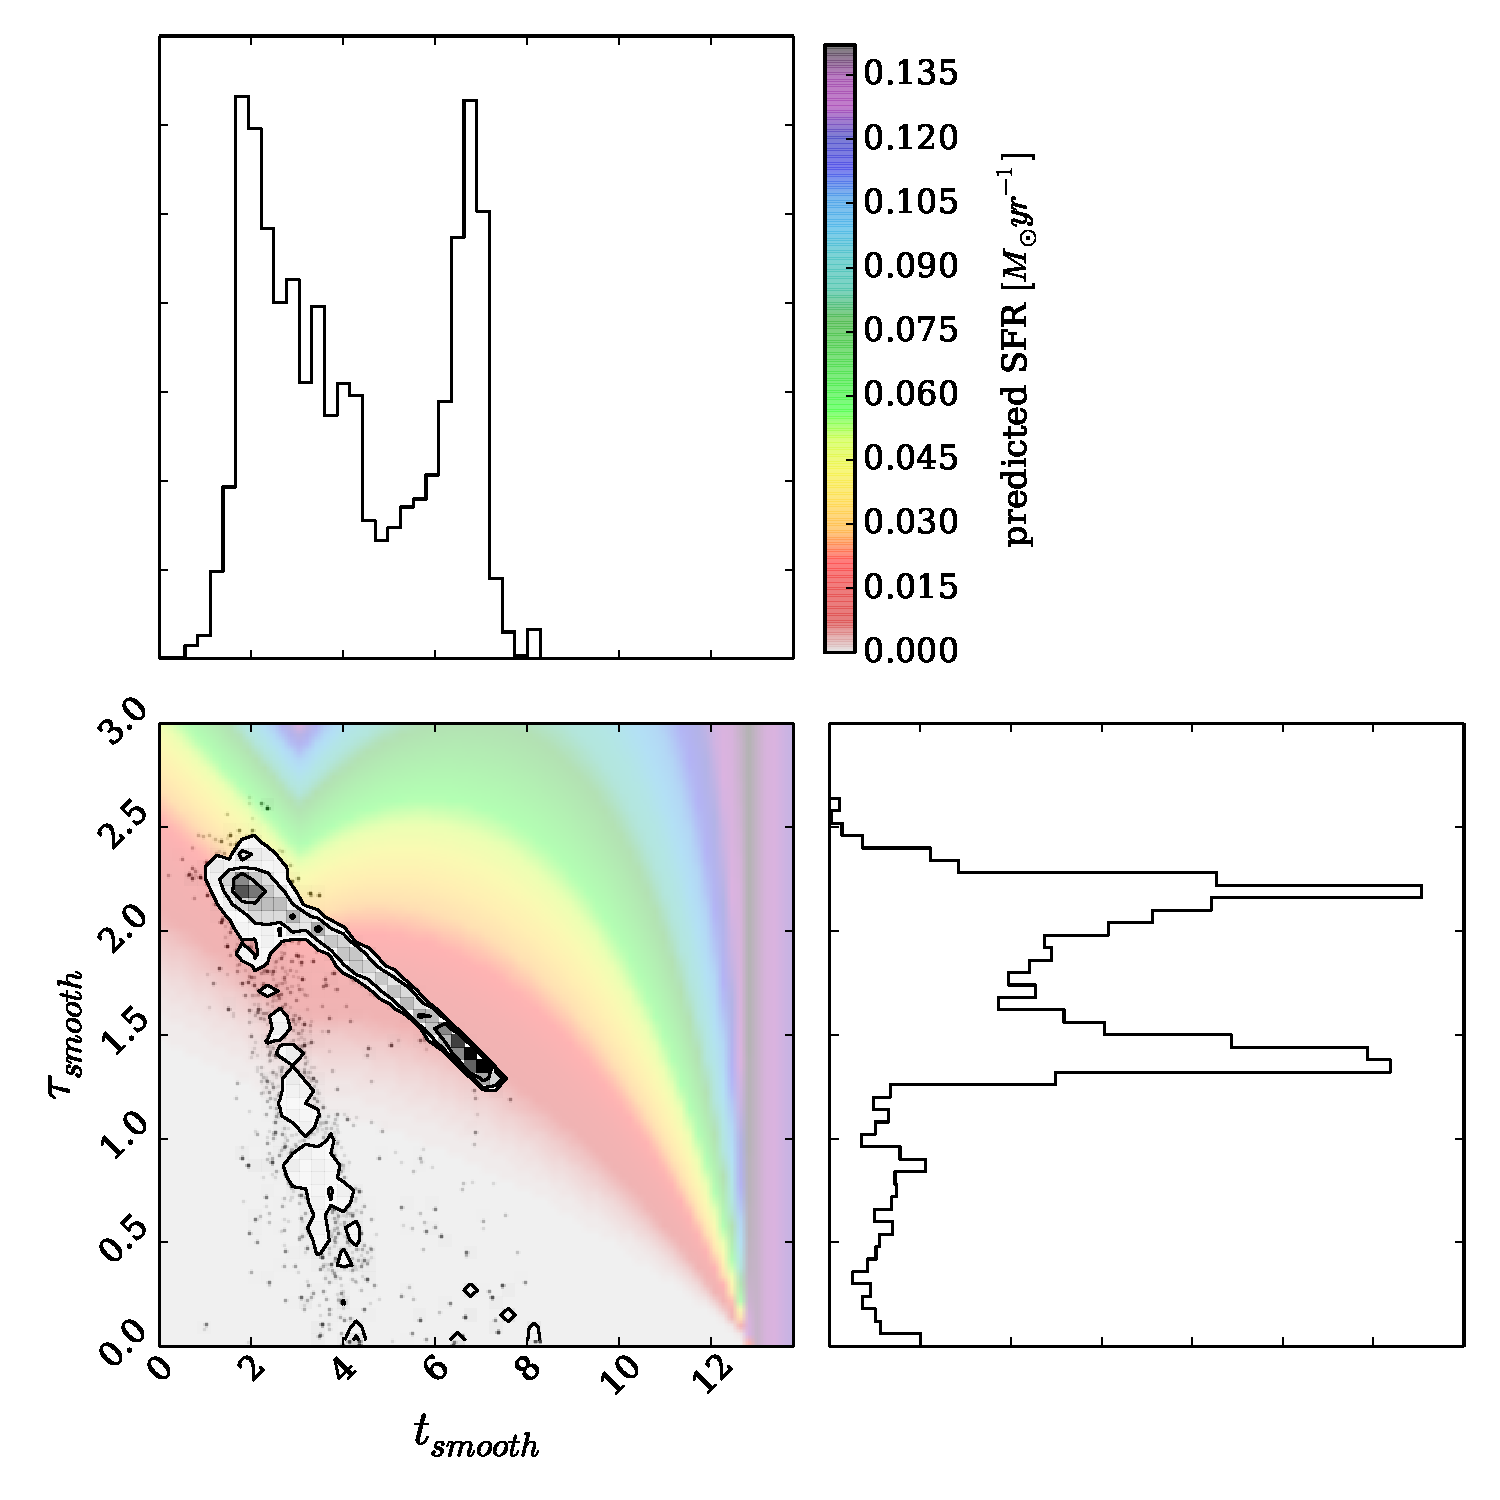
\includegraphics[width=0.4975\textwidth]{red_s_smooth.pdf}
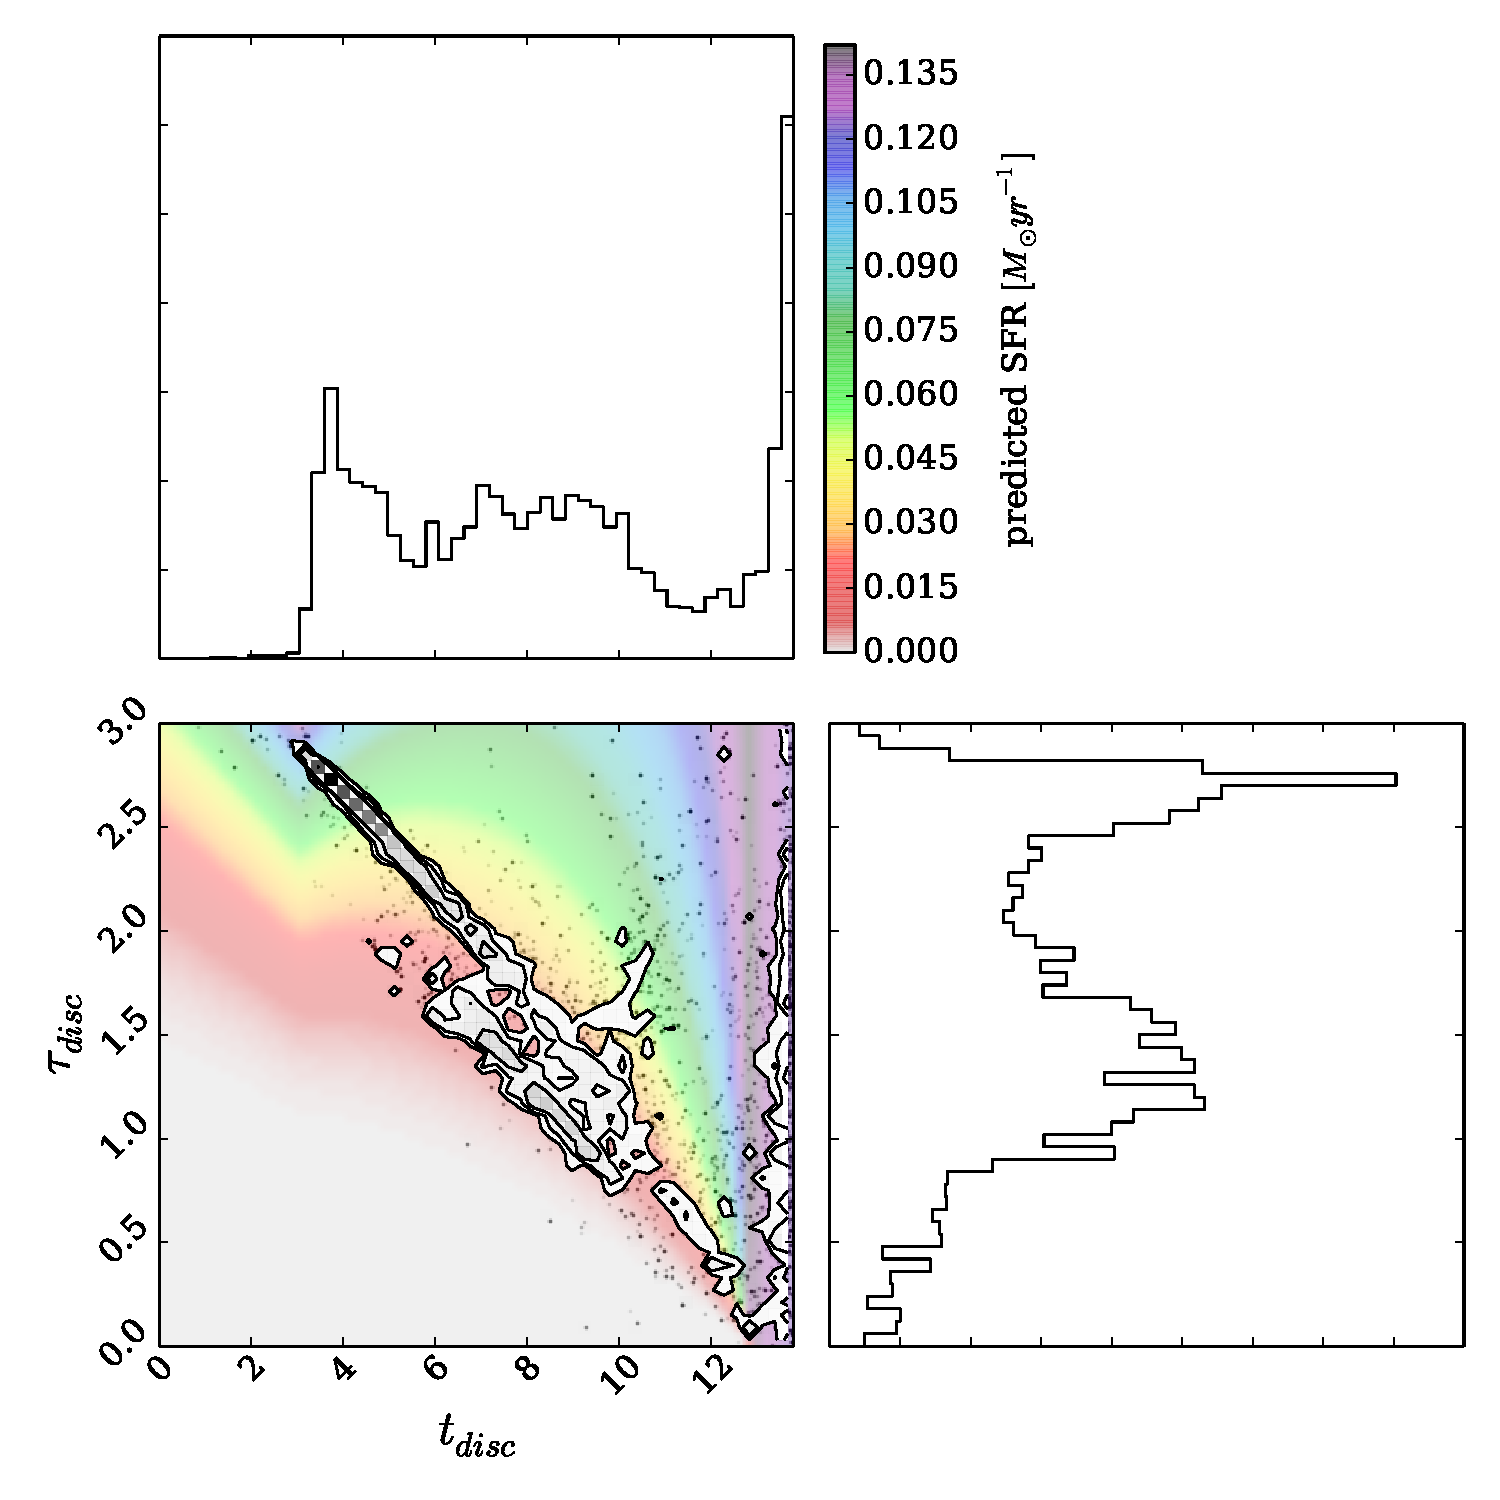
\includegraphics[width=0.4975\textwidth]{red_s_disc.pdf}
\caption[8pt]{Same as for Figure \ref{all} but for galaxies defined as optical Red Sequence \cite{Baldry04}.}
\label{red_s}
\end{figure*}


\begin{figure*}
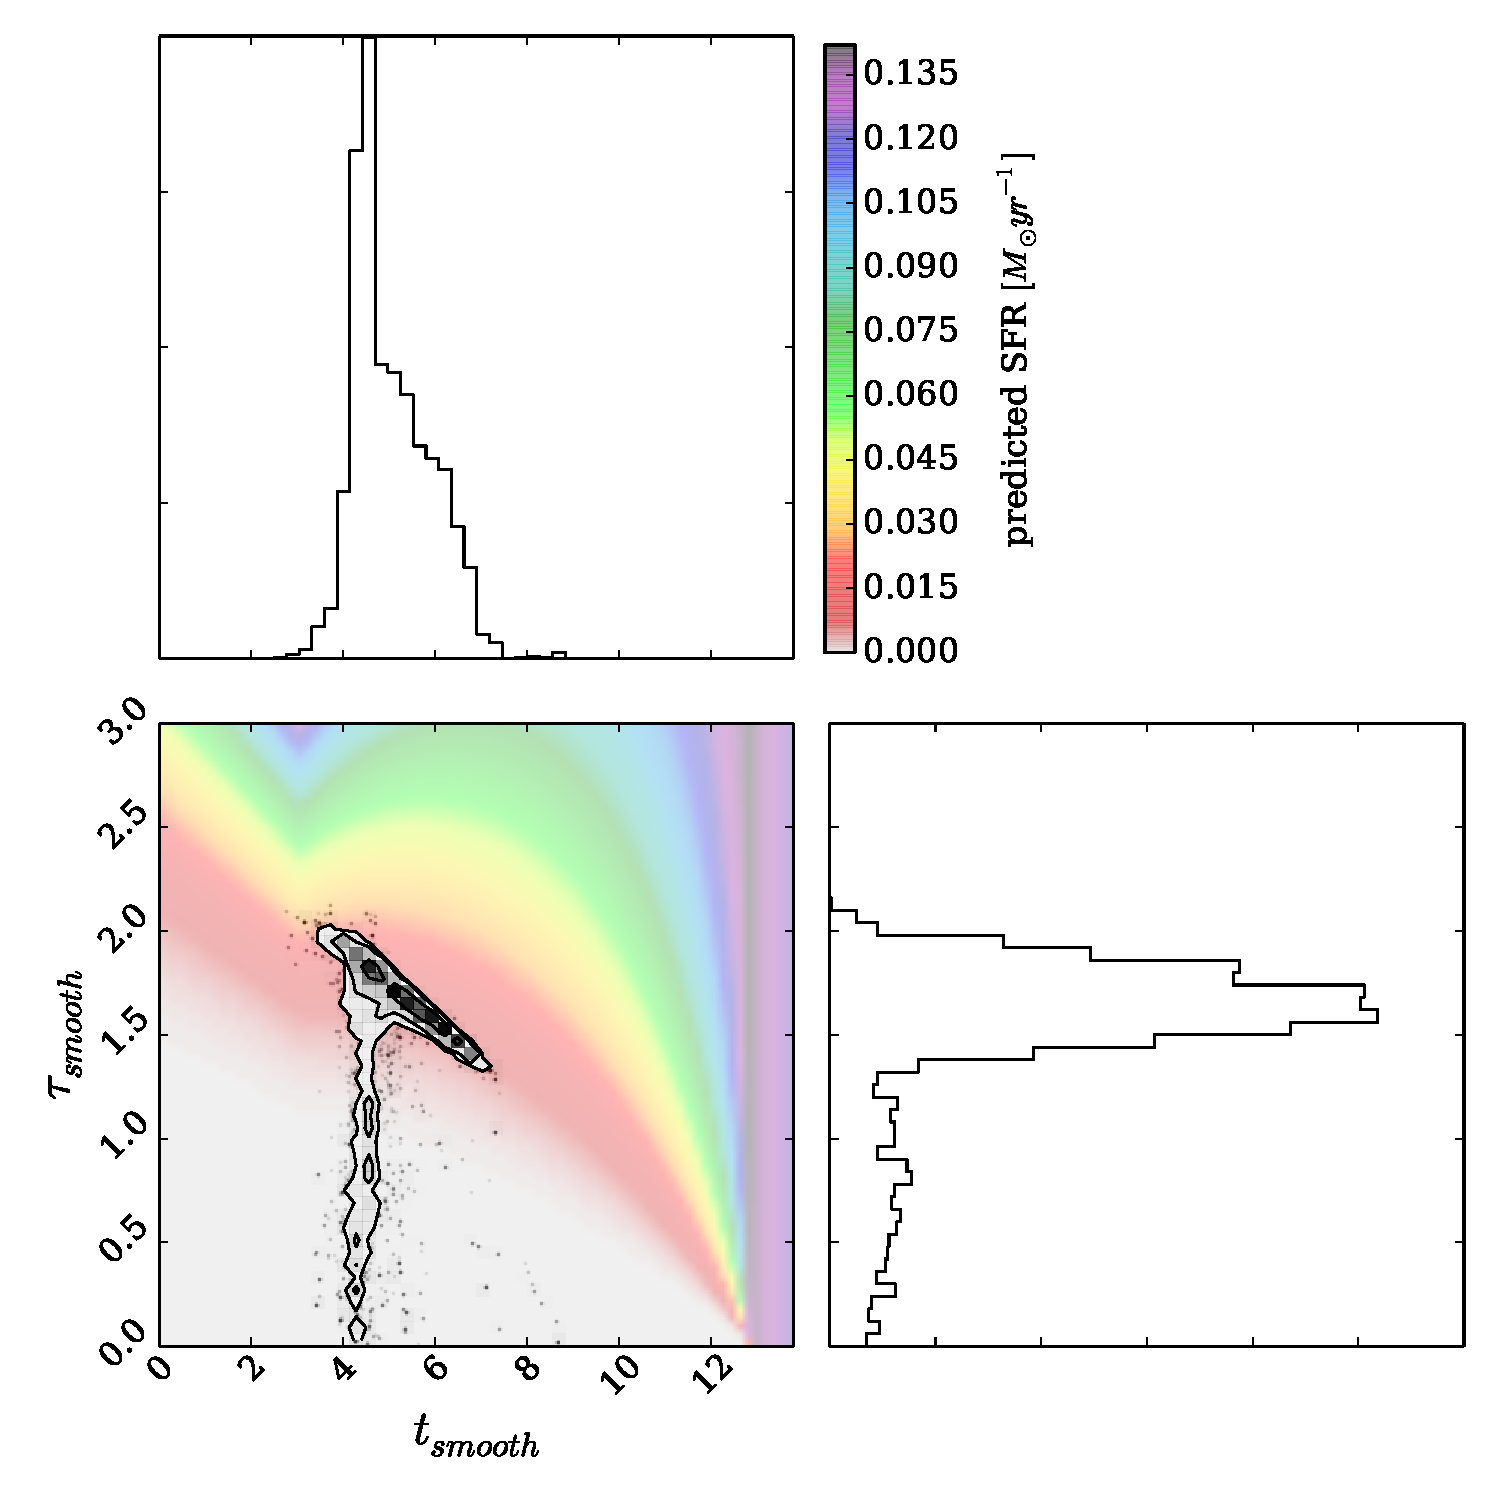
\includegraphics[width=0.4975\textwidth]{red_s_smooth_clean_new.pdf}
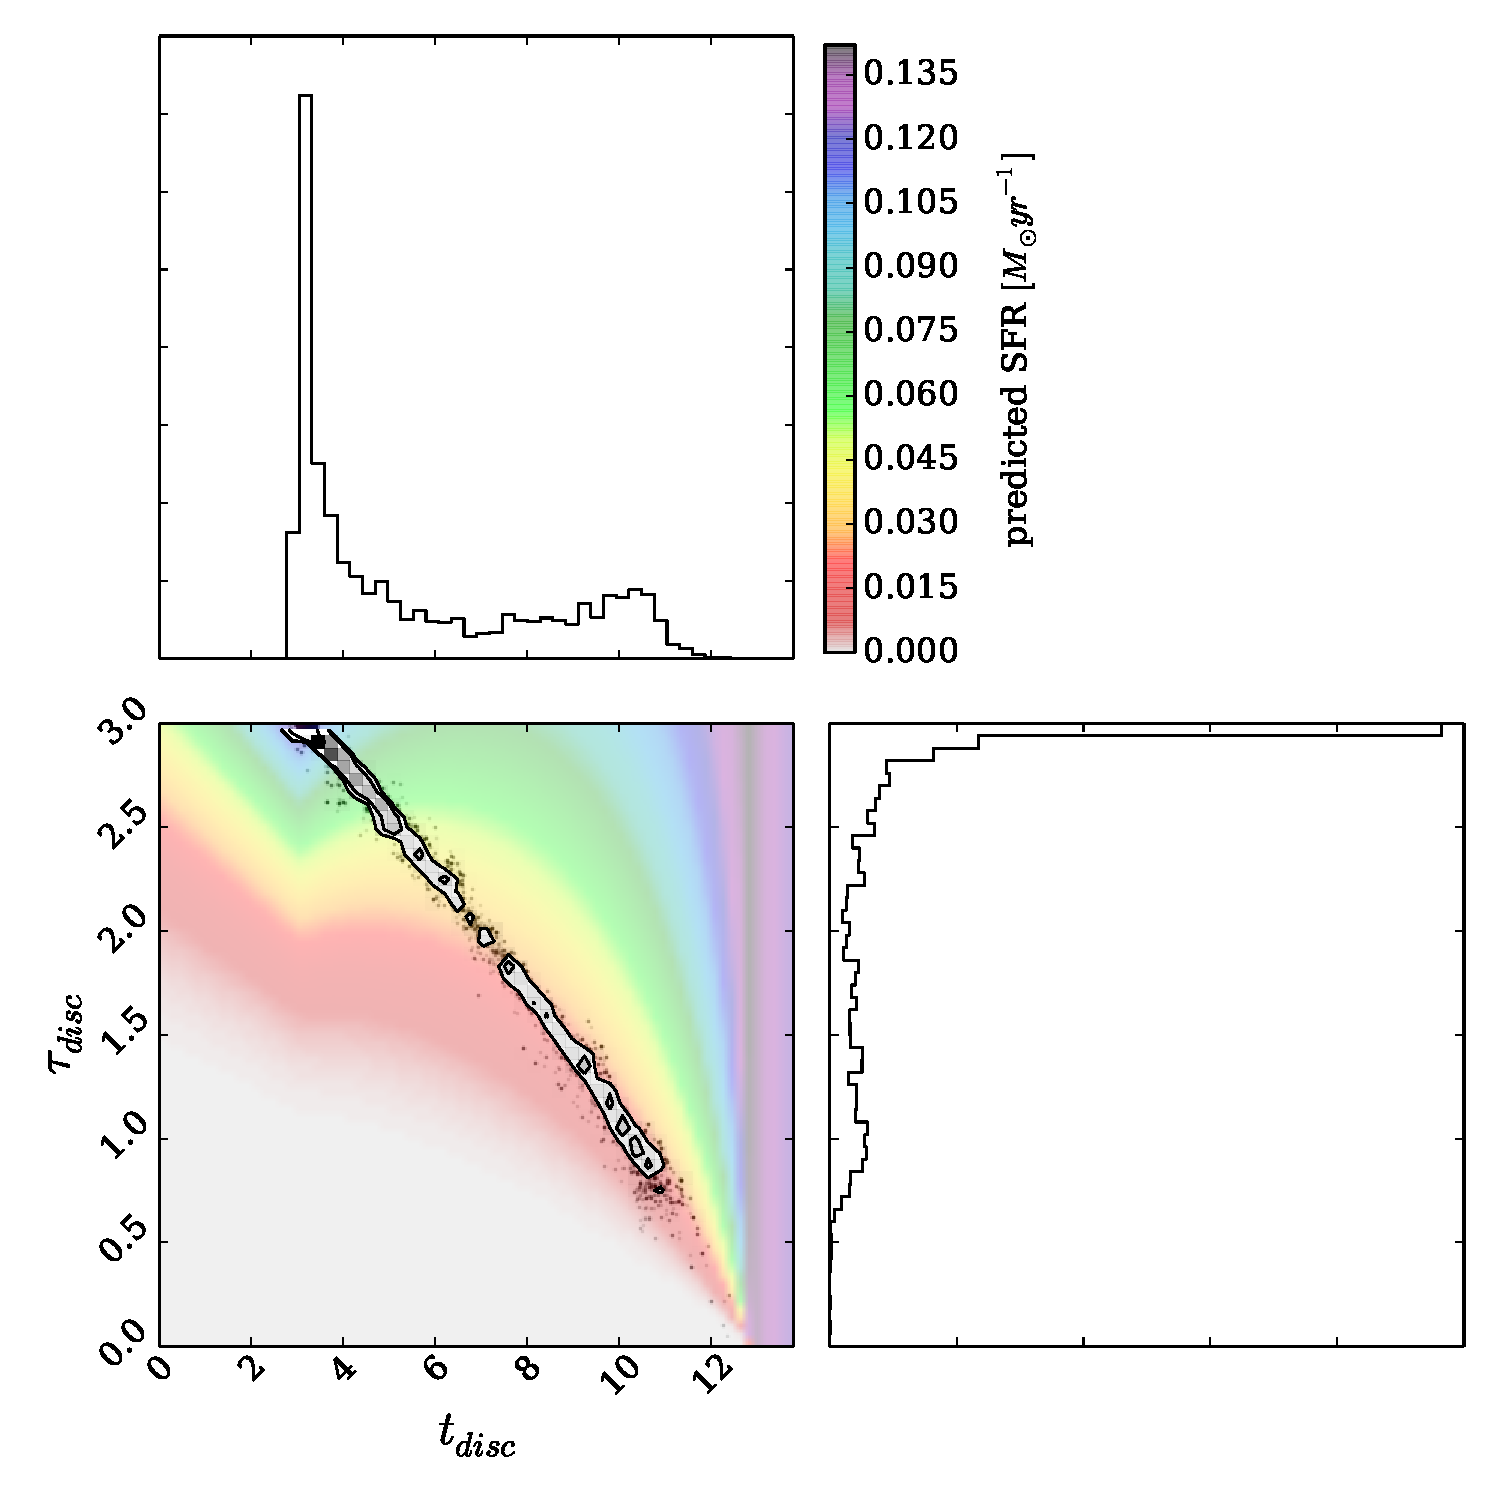
\includegraphics[width=0.4975\textwidth]{red_s_disc_clean_new.pdf}
\caption{Same as for Figure \ref{all} but for galaxies from the clean sample and defined as optical Red Sequence \cite{Baldry04}.}
\label{red_s_clean}
\end{figure*}

\begin{figure*}
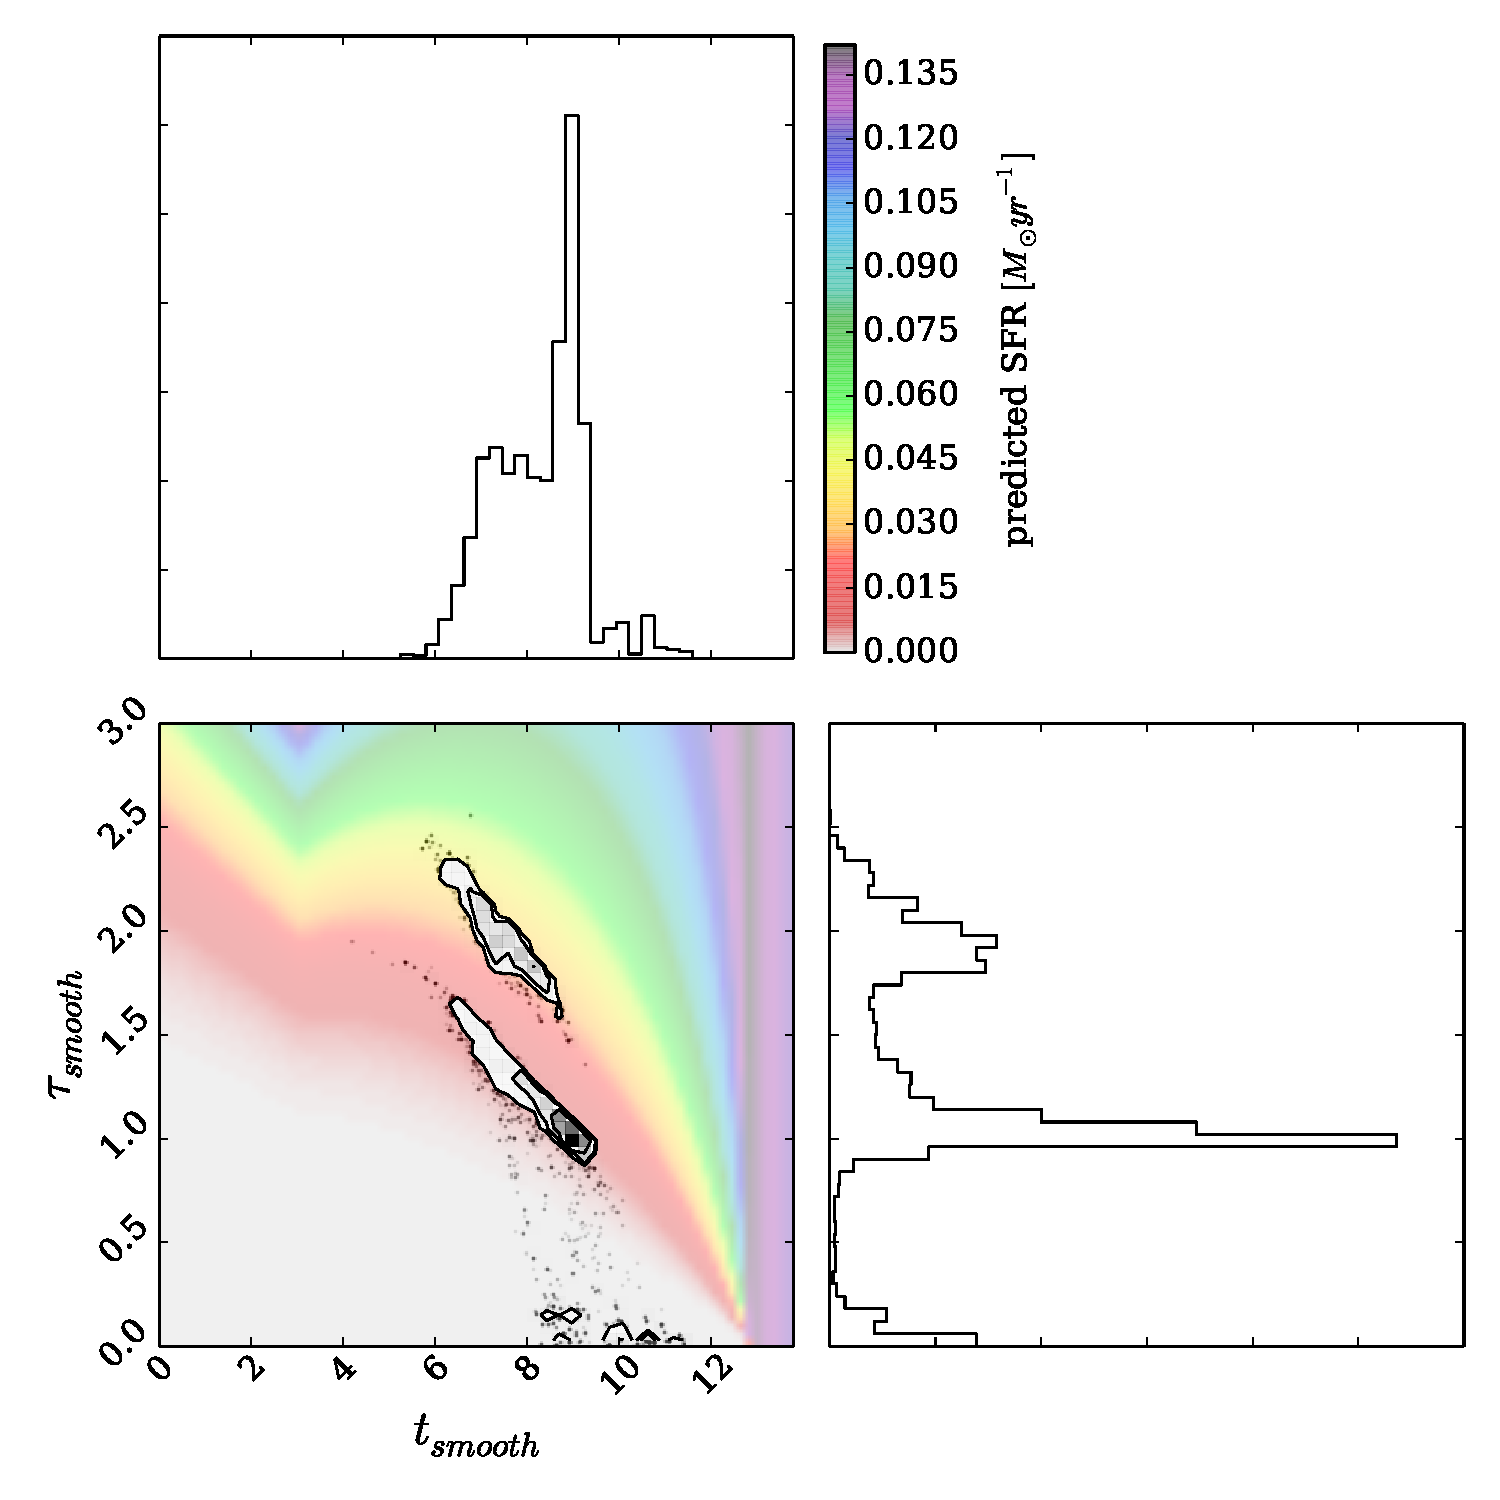
\includegraphics[width=0.4975\textwidth]{gv_smooth.pdf}
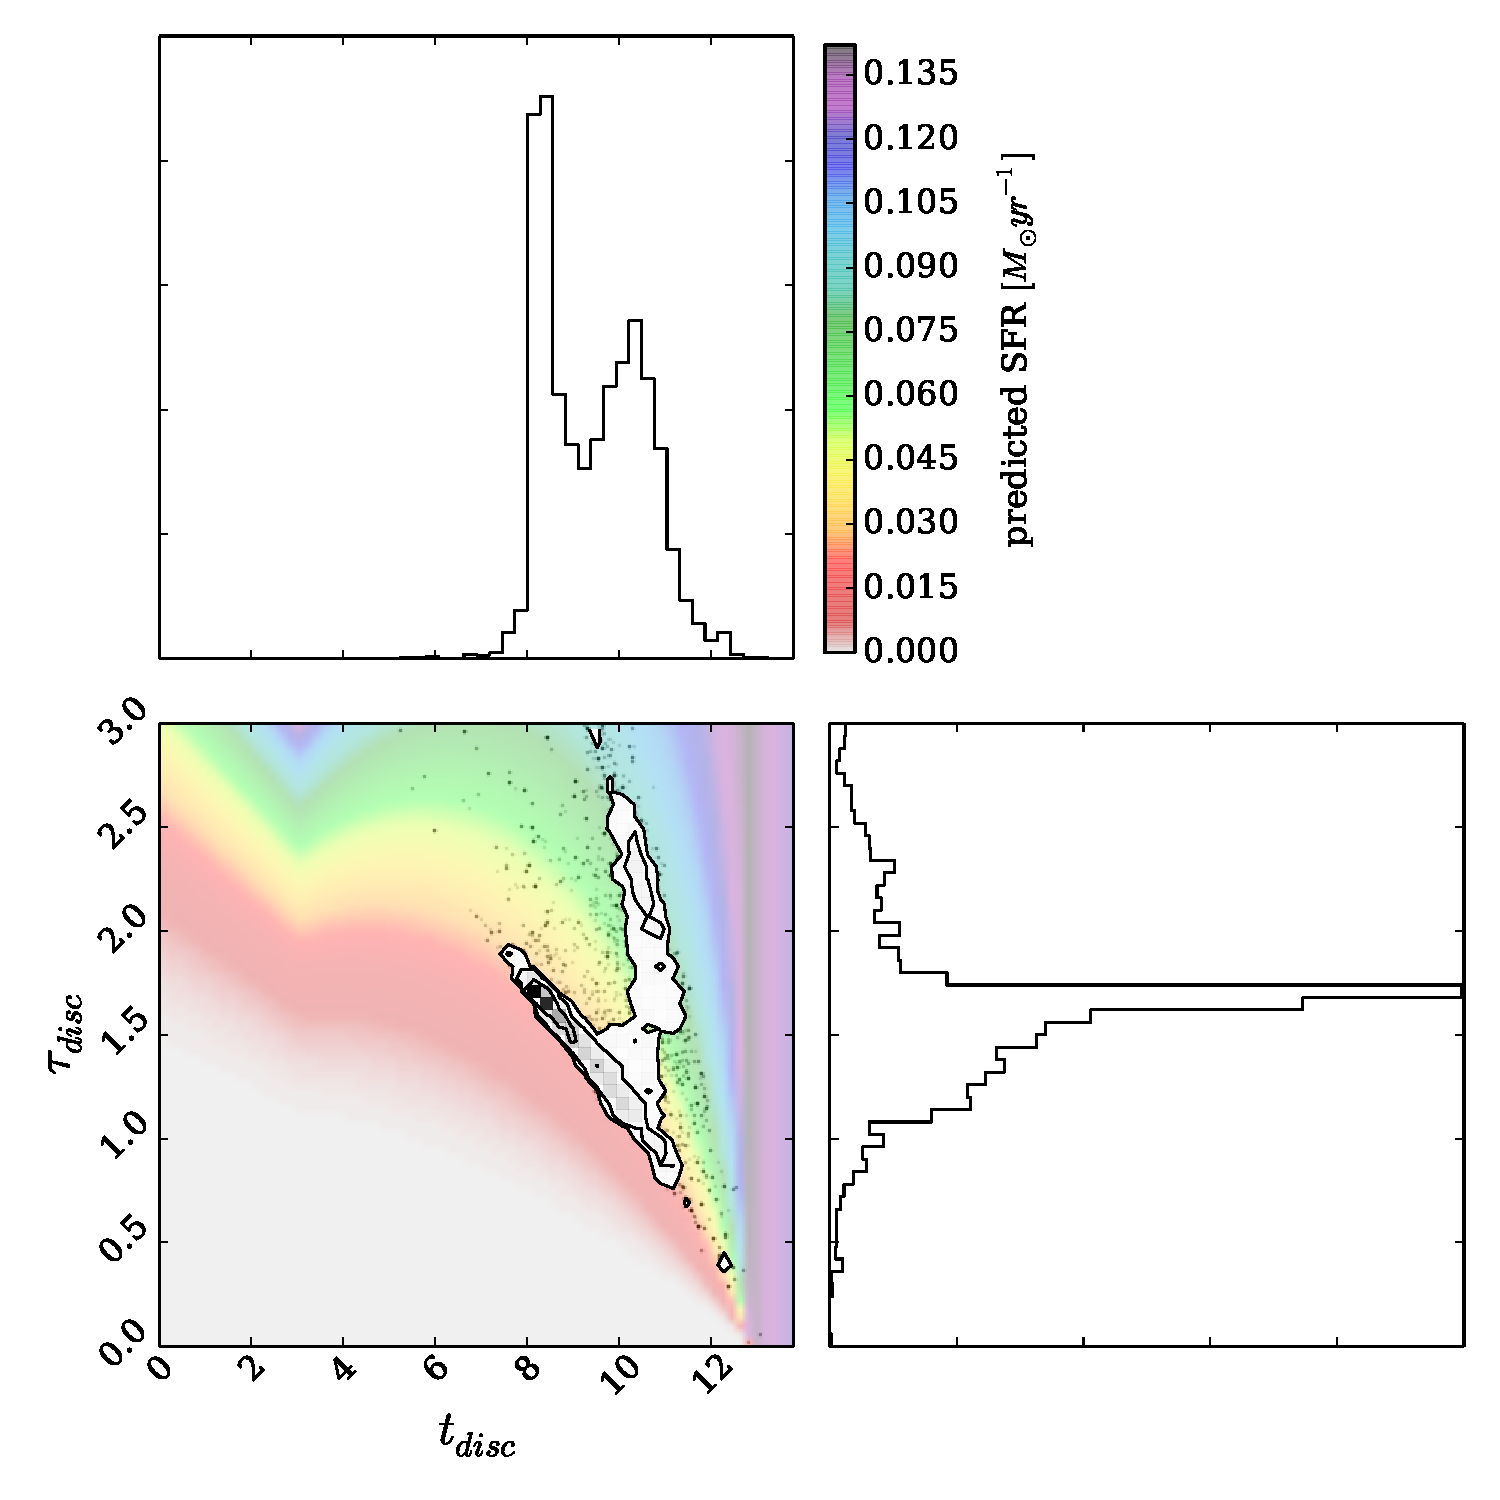
\includegraphics[width=0.4975\textwidth]{gv_disc.pdf}
\caption{Same as for Figure \ref{all} but for galaxies defined as optical Green Valley \cite{Baldry04}.}
\label{gv}
\end{figure*}

\begin{figure*}
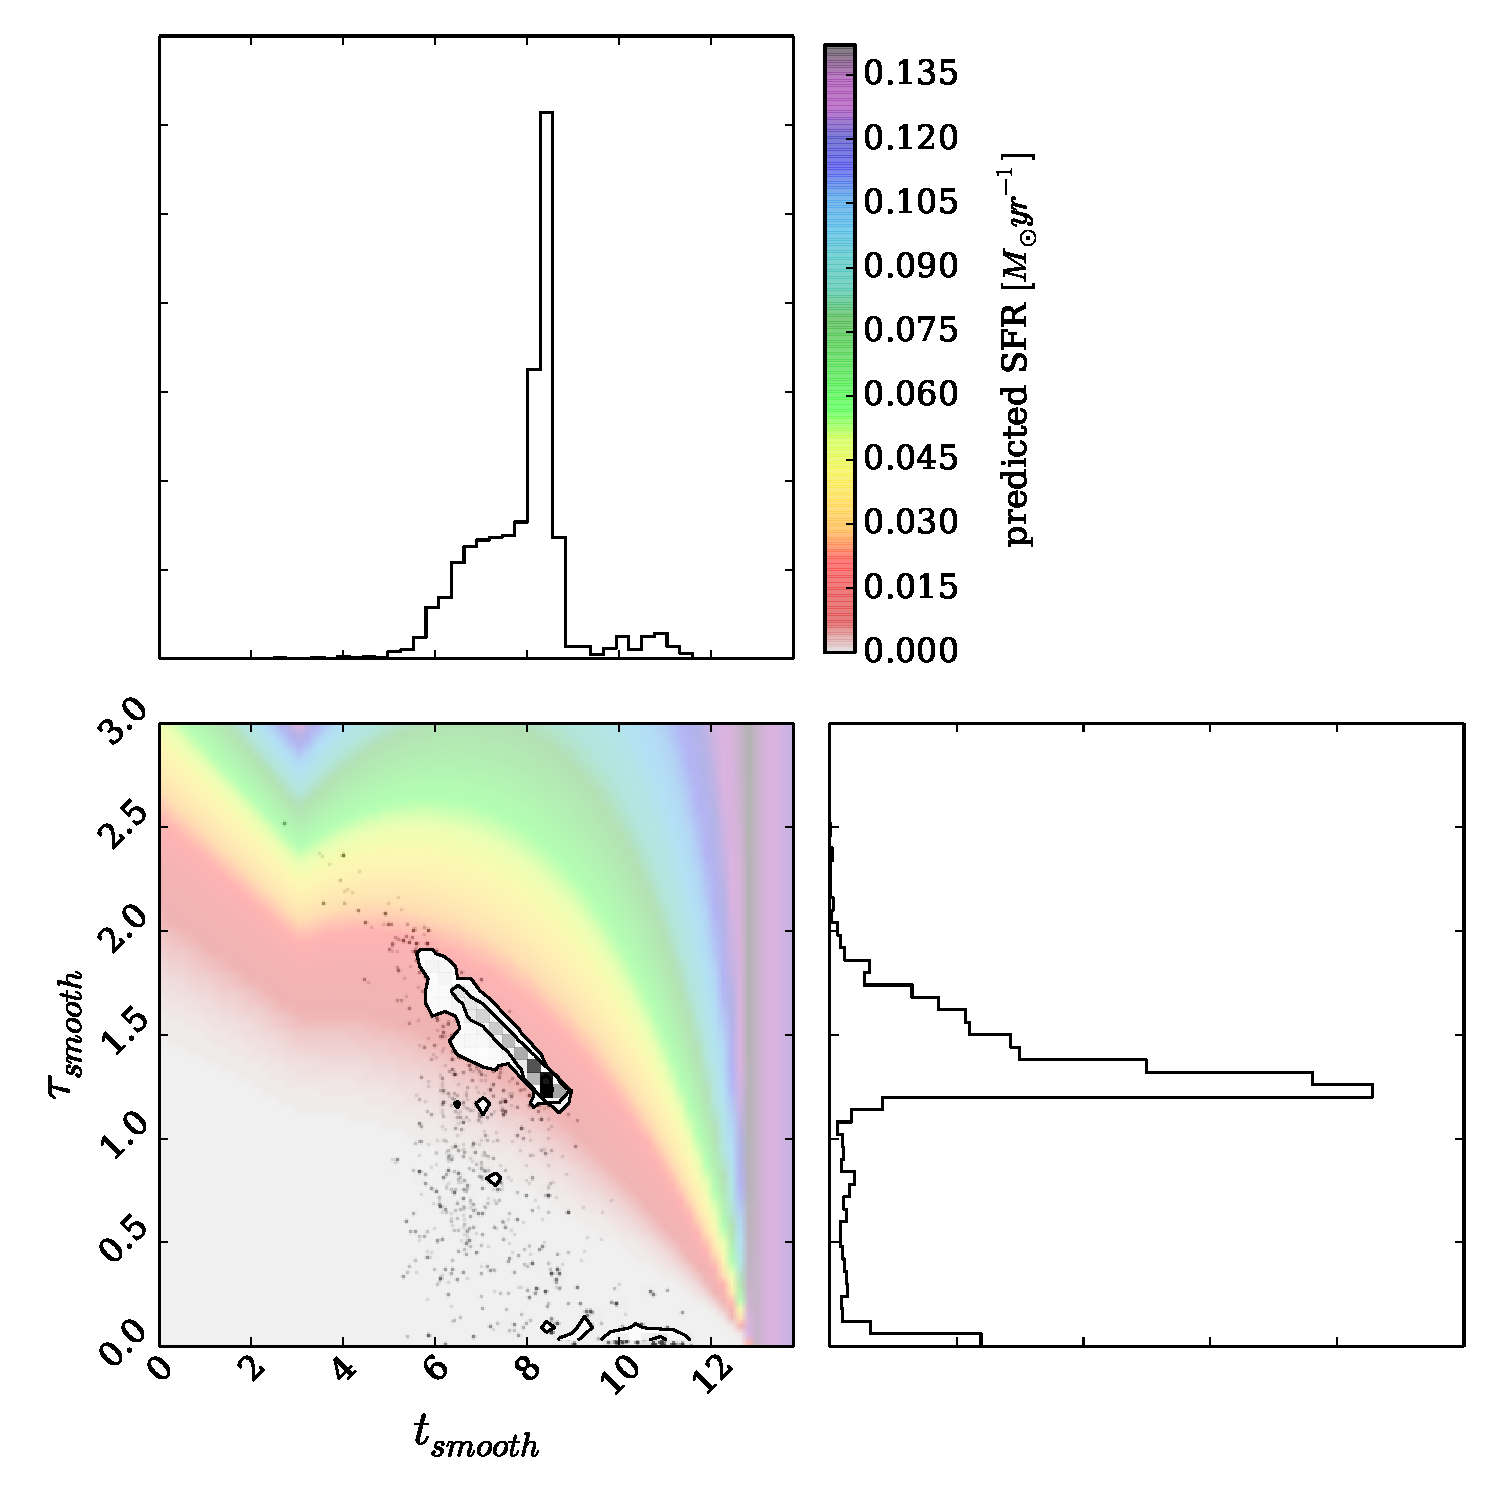
\includegraphics[width=0.4975\textwidth]{gv_smooth_clean.pdf}
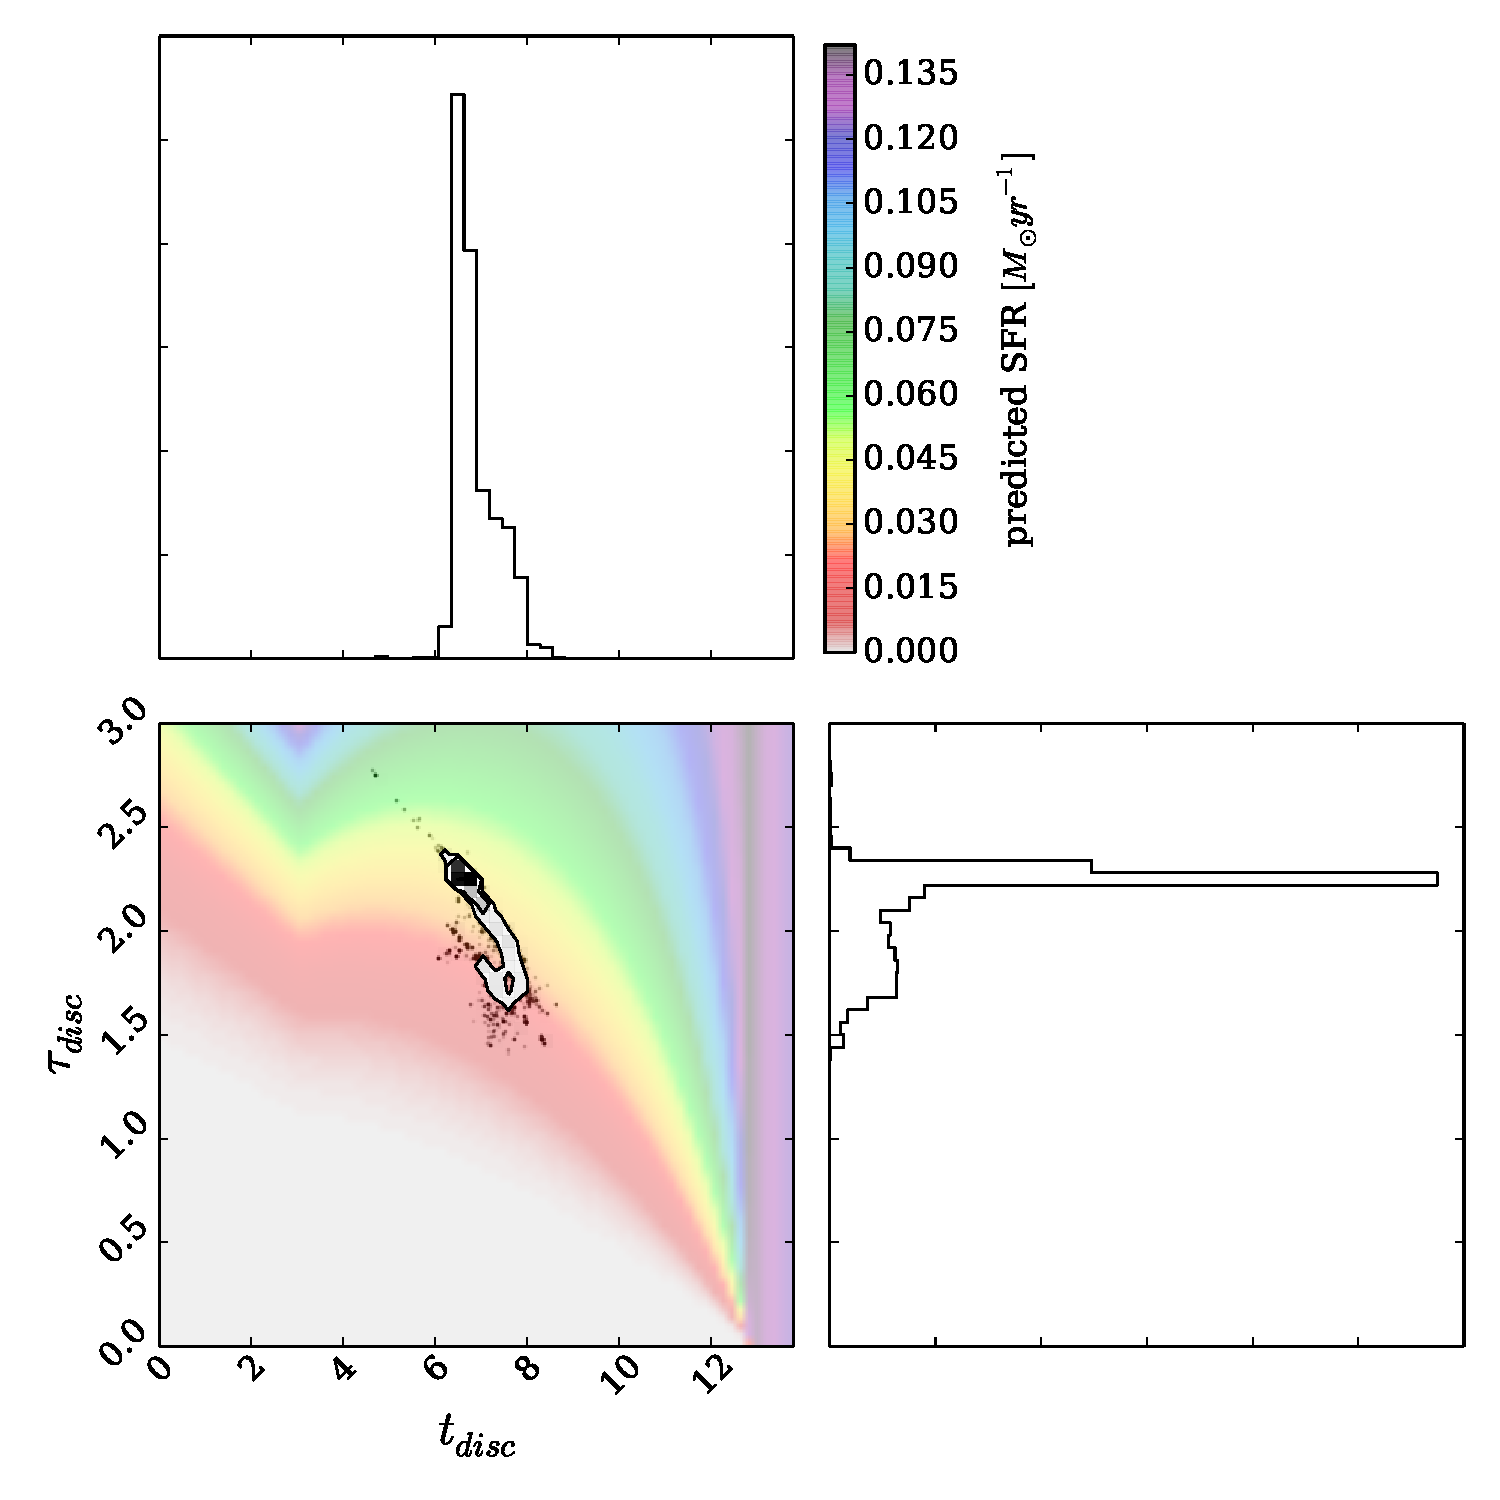
\includegraphics[width=0.4975\textwidth]{gv_disc_clean.pdf}
\caption{Same as for Figure \ref{all} but for galaxies from the clean sample and defined as optical Green Valley \cite{Baldry04}.}
\label{gv_clean}
\end{figure*}

\begin{figure*}
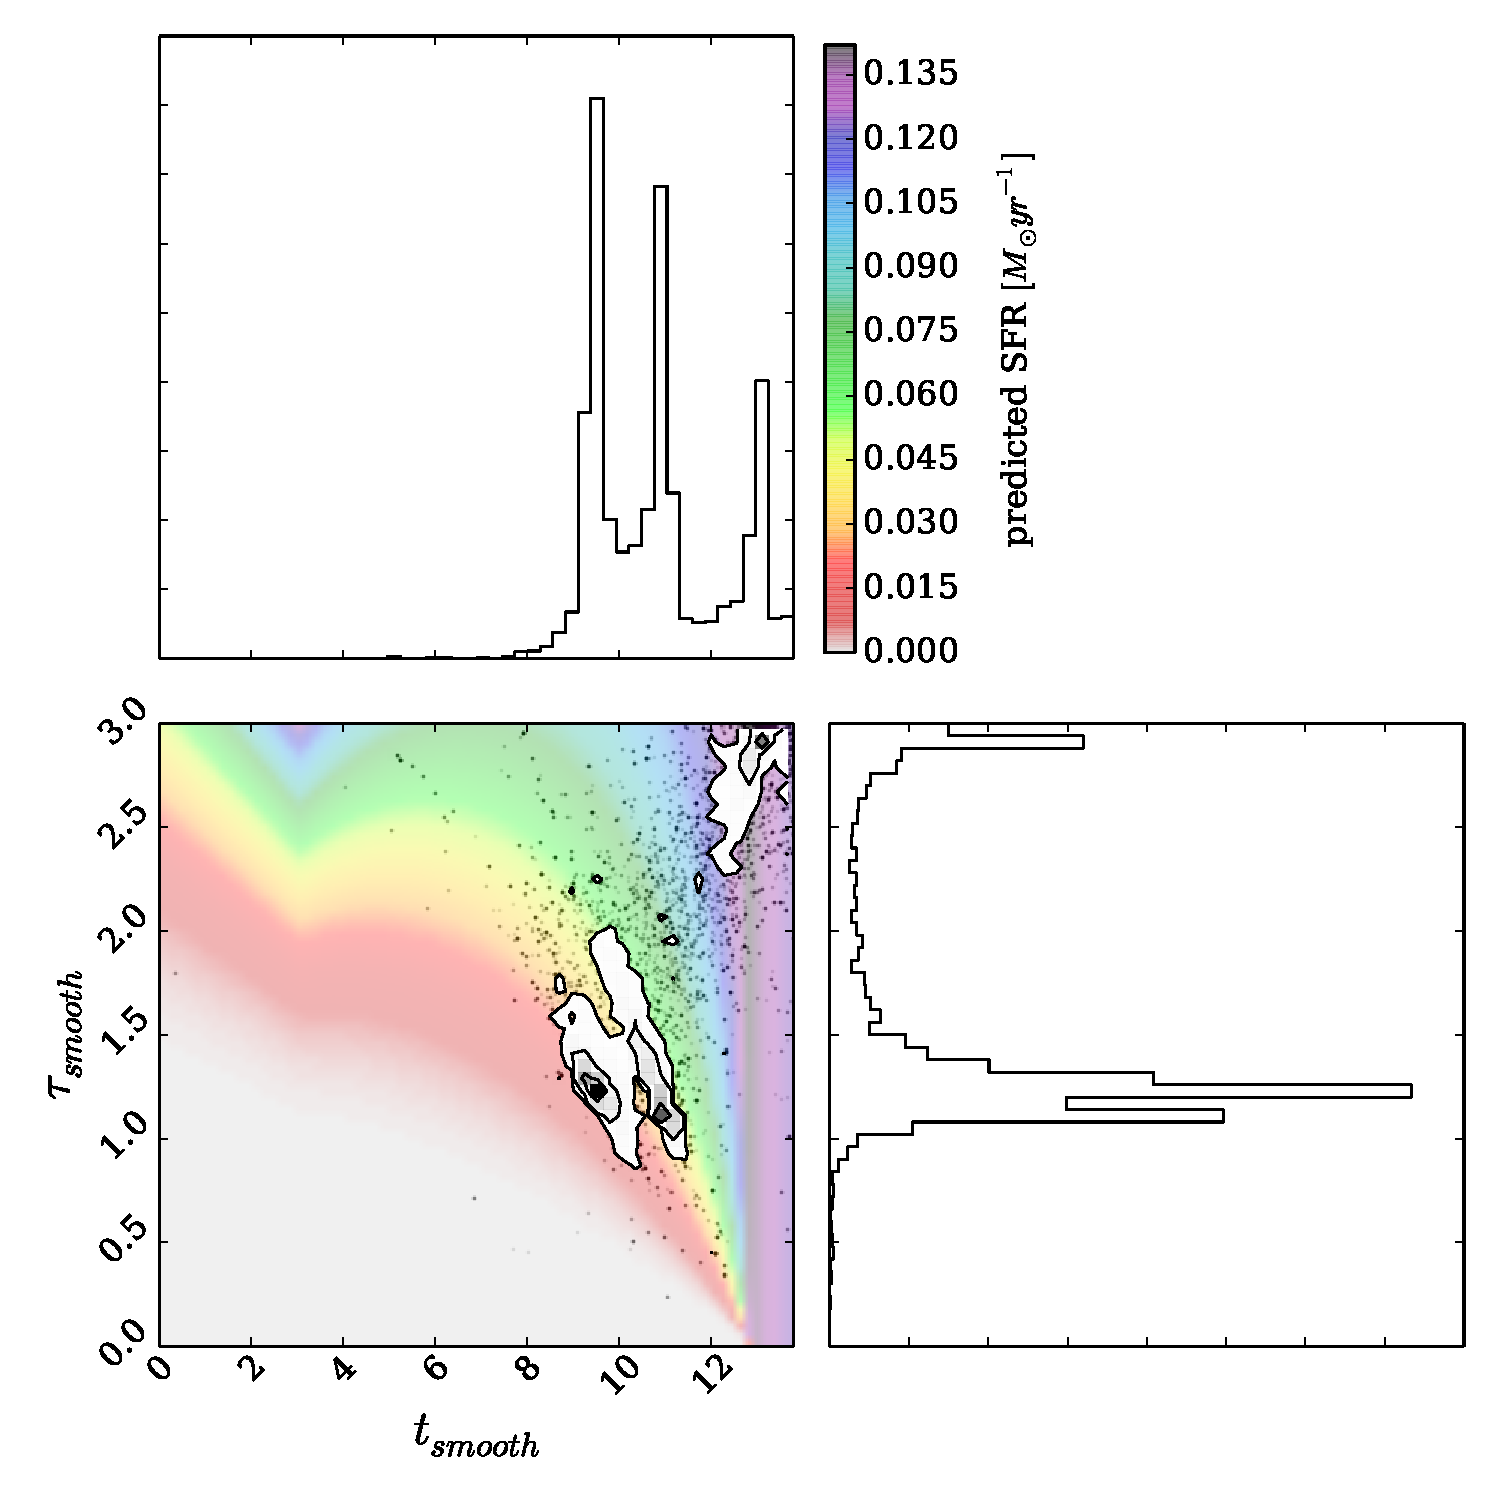
\includegraphics[width=0.4975\textwidth]{blue_c_smooth.pdf}
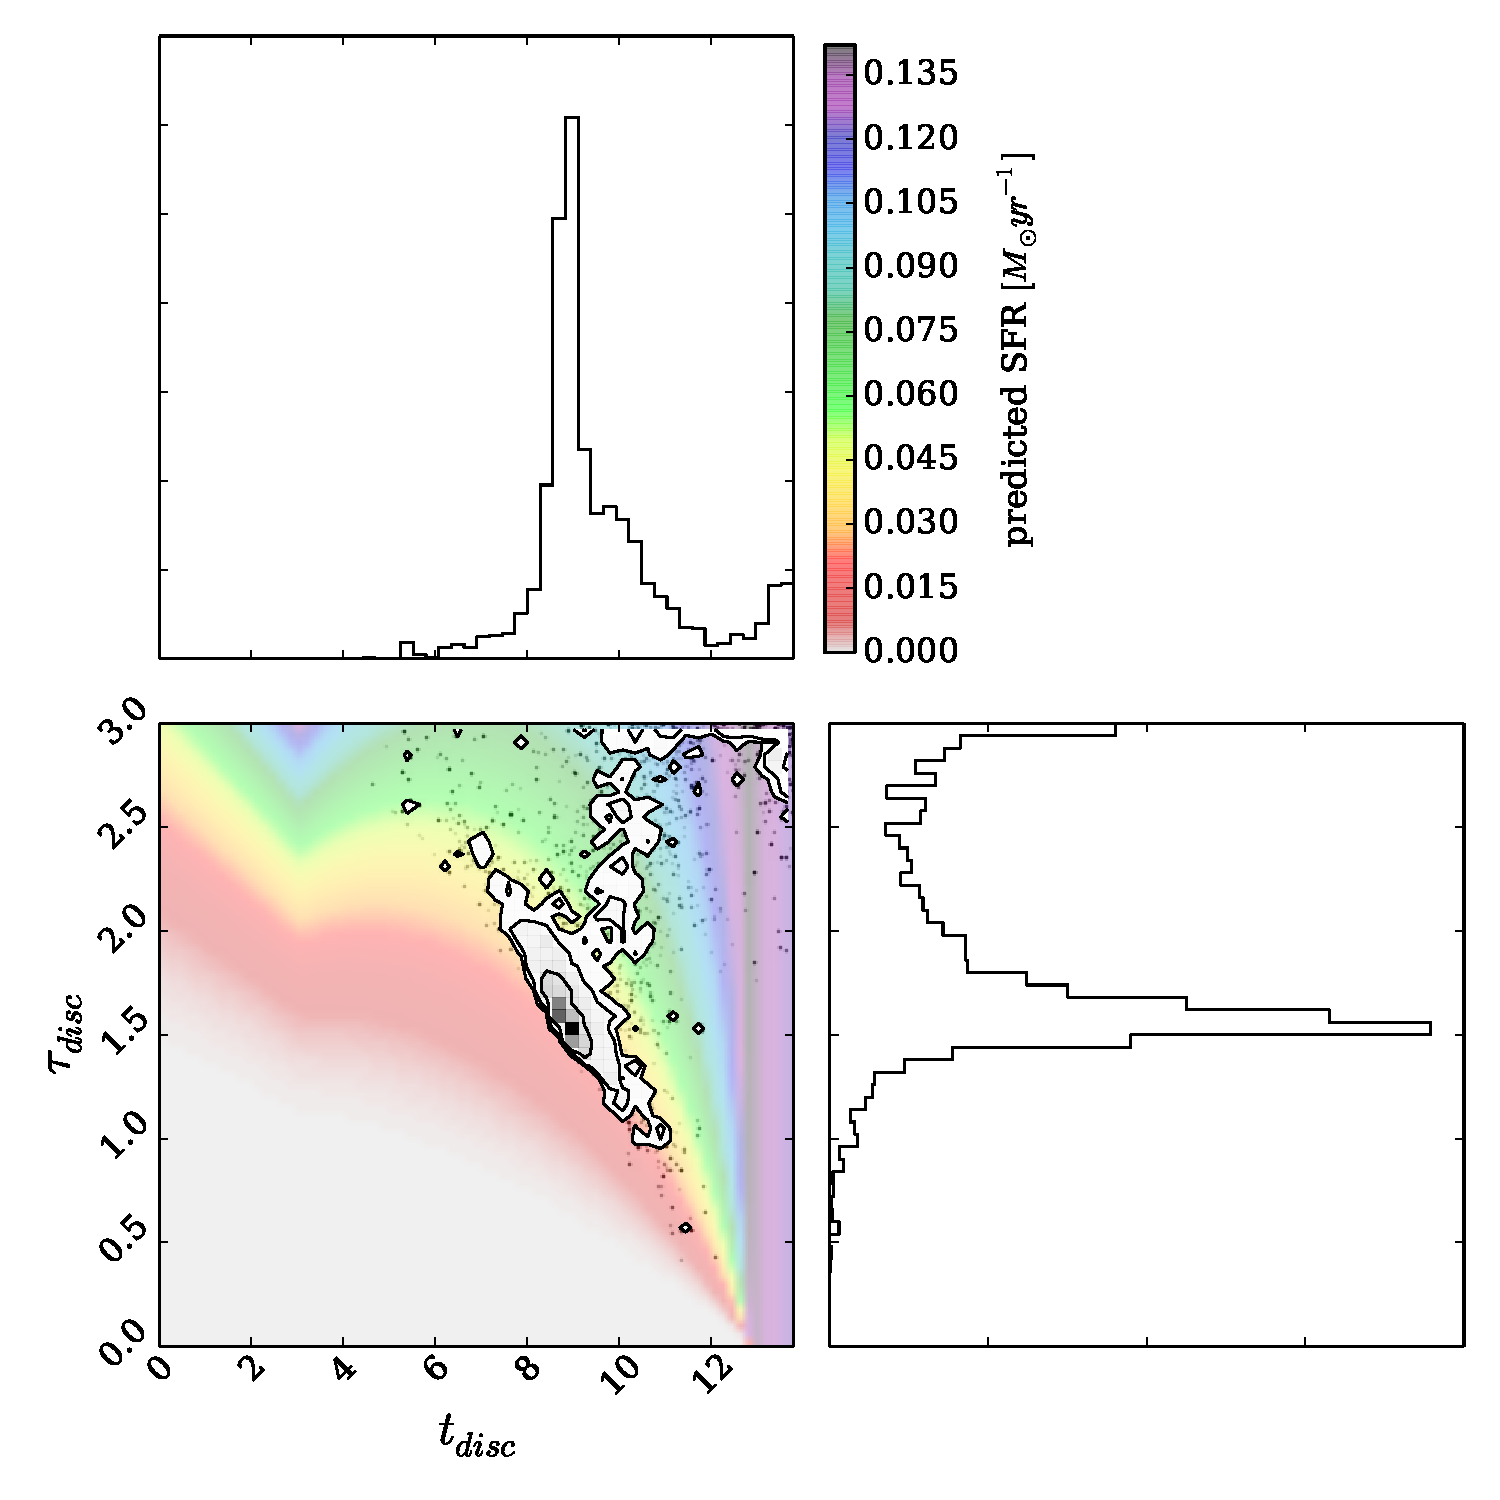
\includegraphics[width=0.4975\textwidth]{blue_c_disc.pdf}
\caption{Same as for Figure \ref{all} but for galaxies defined as optical Blue Cloud \cite{Baldry04}.}
\label{blue_c}
\end{figure*}

\begin{figure*}
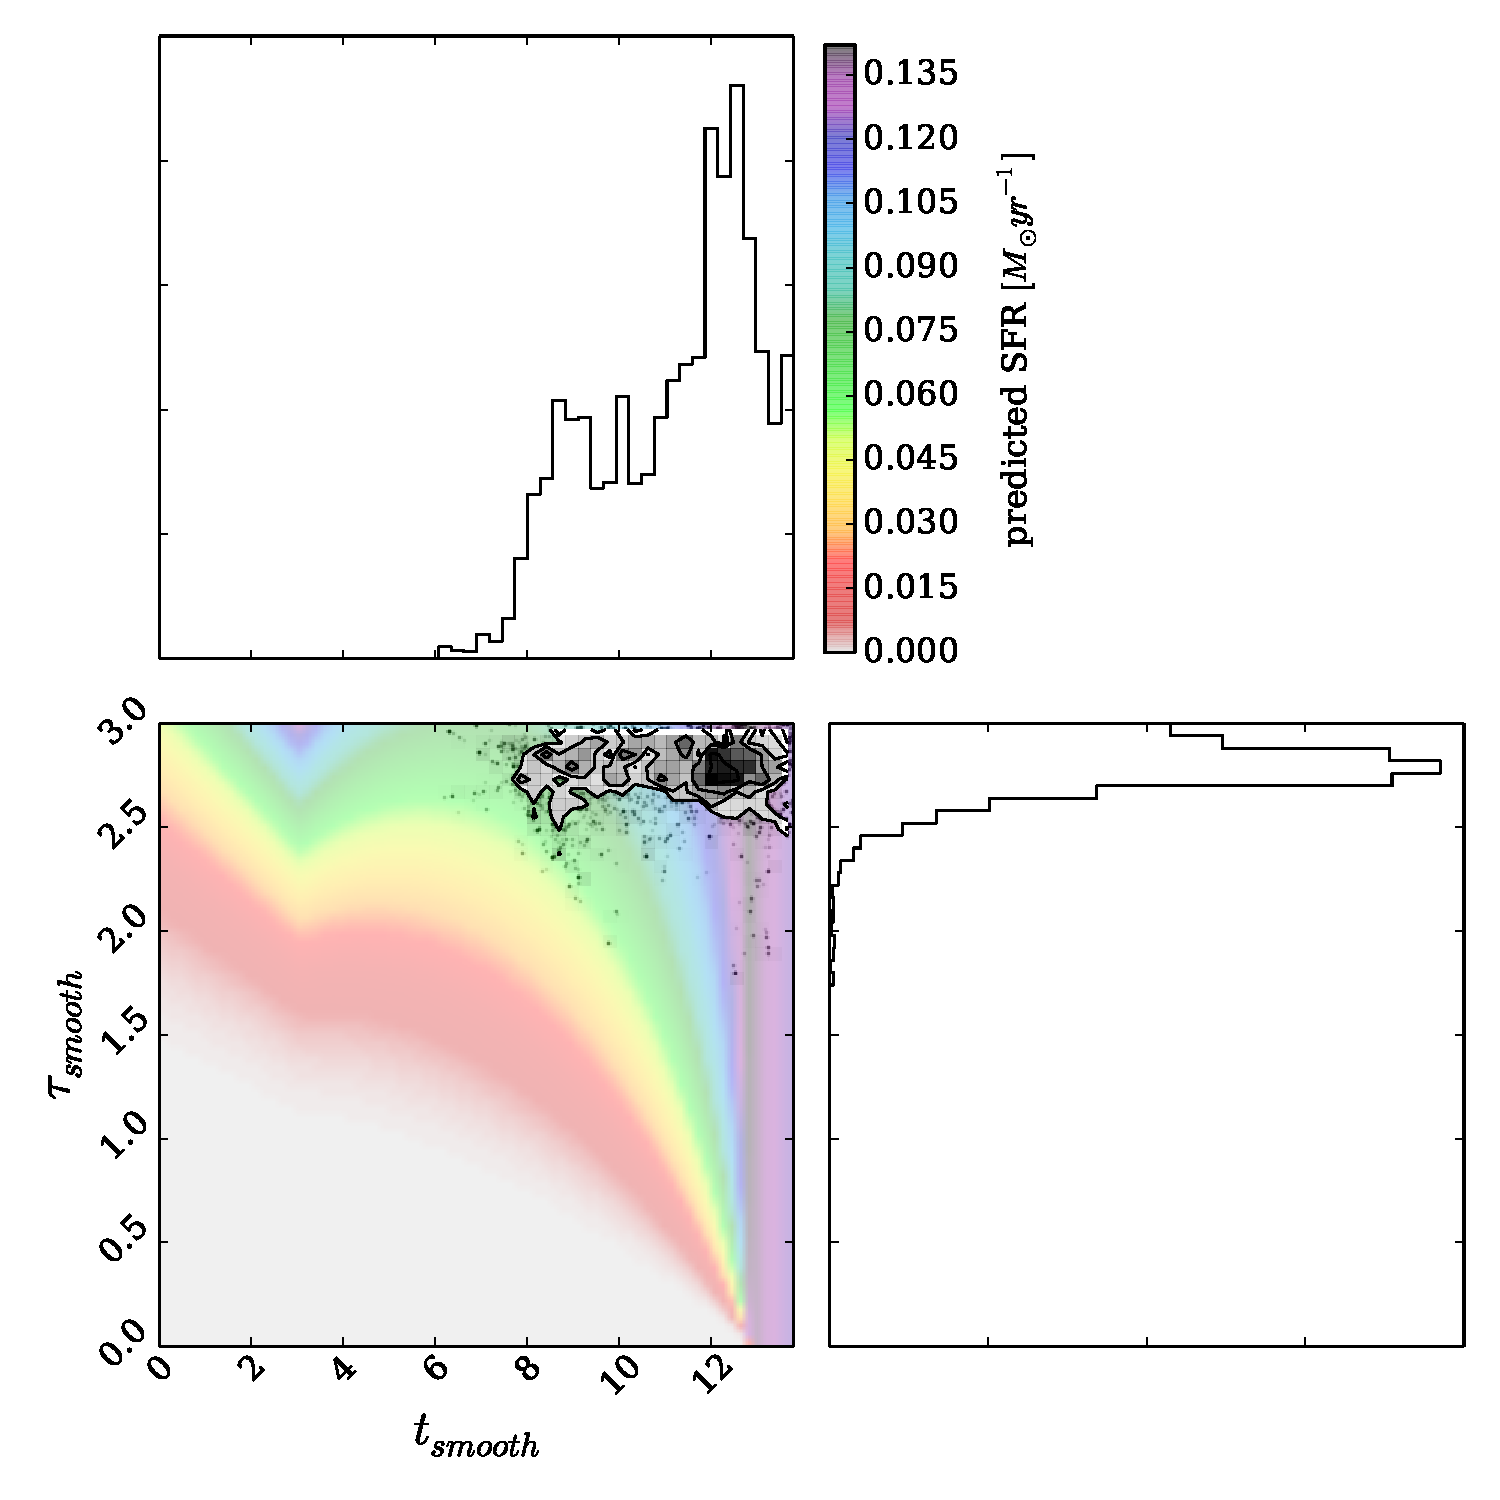
\includegraphics[width=0.4975\textwidth]{blue_c_smooth_clean.pdf}
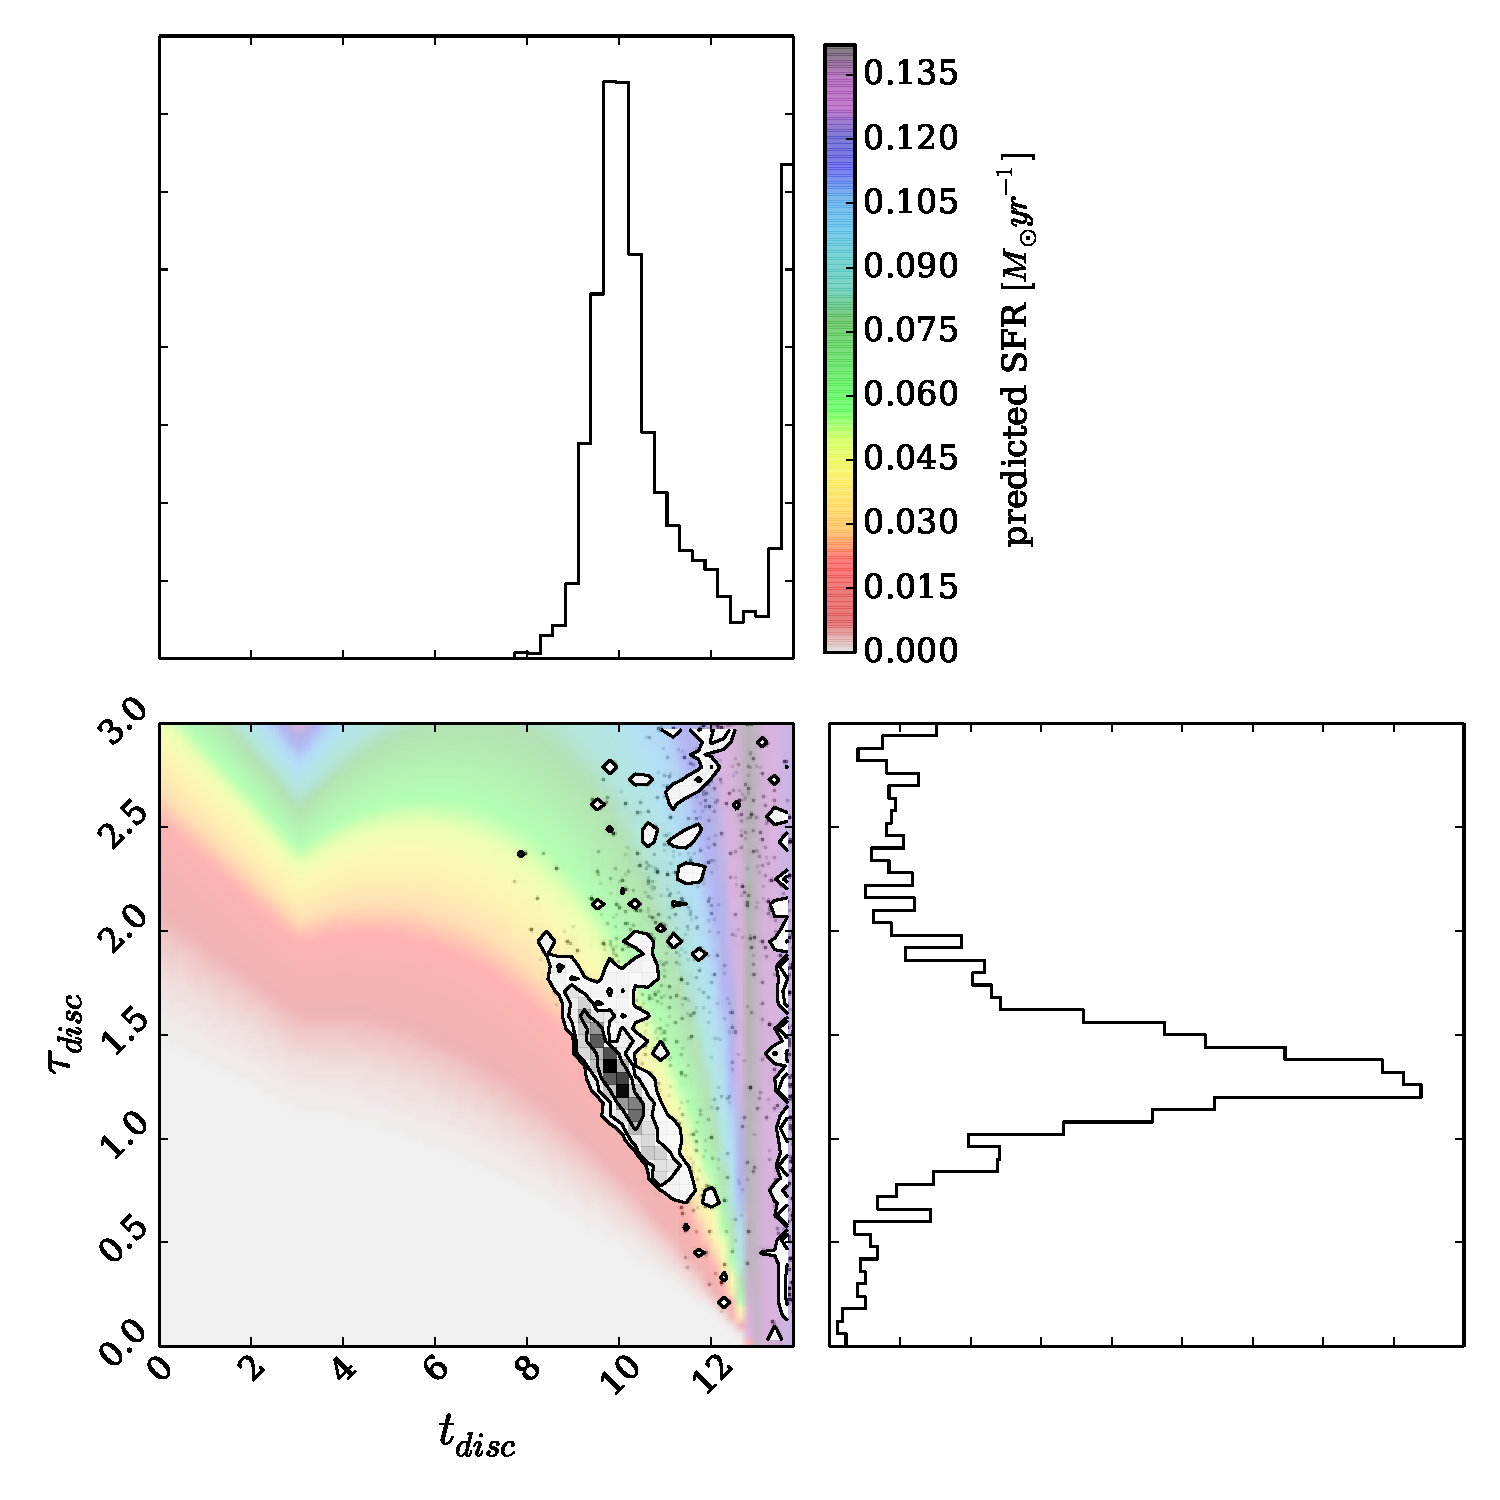
\includegraphics[width=0.4975\textwidth]{blue_c_disc_clean.pdf}
\caption{Same as for Figure \ref{all} but for galaxies from the clean sample and defined as optical Blue Cloud \cite{Baldry04}.}
\label{blue_c_clean}
\end{figure*}

In figure \ref{all} we can immediately see that the two populations occupy very different locations in the $\theta$ parameter space supporting the conclusion in \citet{Sch2014} that early- and late- type galaxies quench on different timescales. For the disk-like galaxies we can also see a significant \emph{correlation} between the two parameters $t$ and $\tau$ (if quenching occurs earlier, then the quenching timescale increases). Perhaps this is due to a dependancy on the environment which galaxies occupied at earlier times compared to later times. 

For the disc-like galaxies we have a bimodal likelihood in the SFH parameter space, whereas for the smooth-like galaxies we have a trimodal likelihood. For the disc galaxies we see no likelihood below $\tau \sim 1~Gyr$ (rapid quenching; the right panel of figure \ref{sfr_mass_col} shows models with $\tau \leq 1.0~Gyr$ reside in the red sequence within $\sim 3~Gyr$), whereas we do see an area of likelihood for the smooth galaxies - most likely caused by typical `red and dead' early type galaxies. The areas of high likelihood for $t$ for the disc-like galaxies also span a much larger range than for the smooth-like galaxies.


\subsection{Red Sequence Galaxies}


%\begin{figure*}
%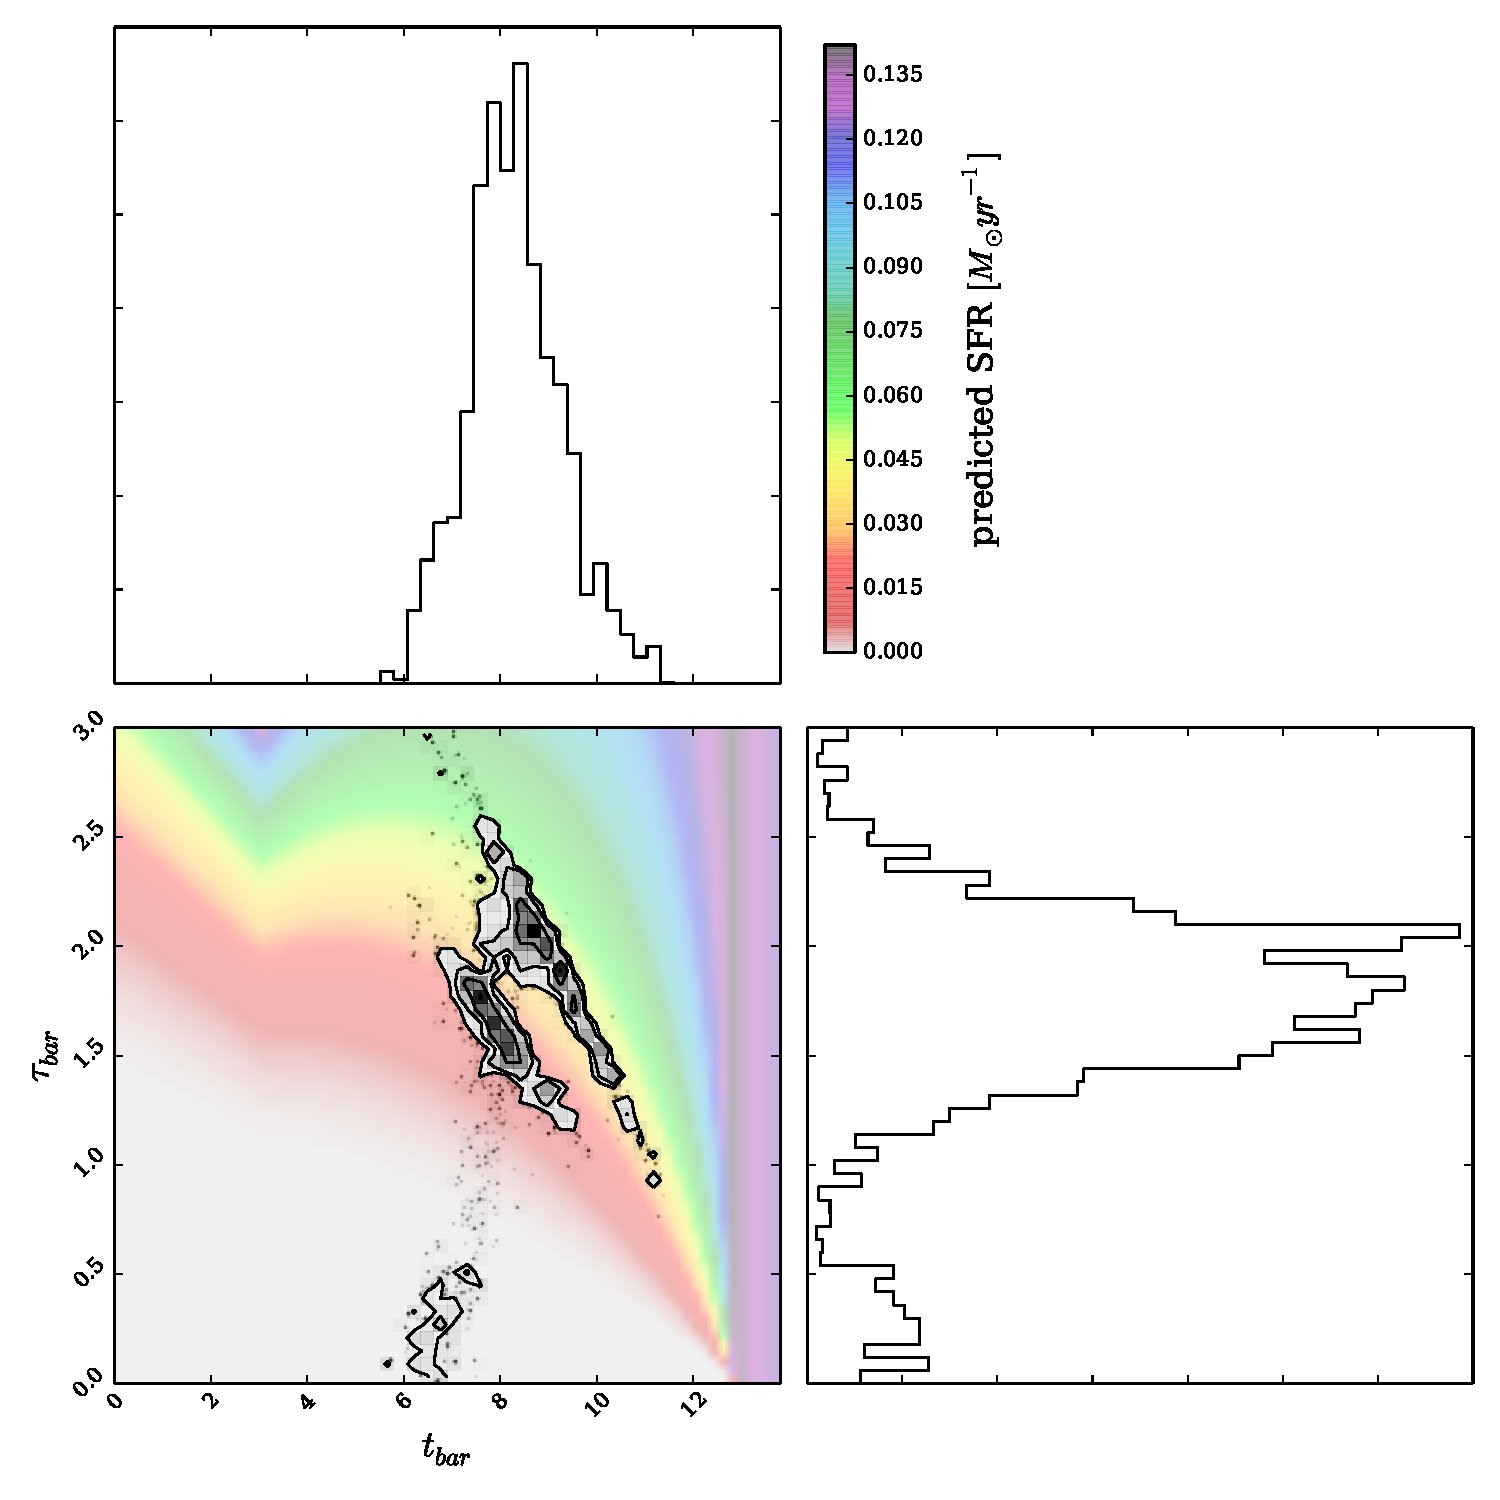
\includegraphics[width=0.4975\textwidth]{bars.pdf}
%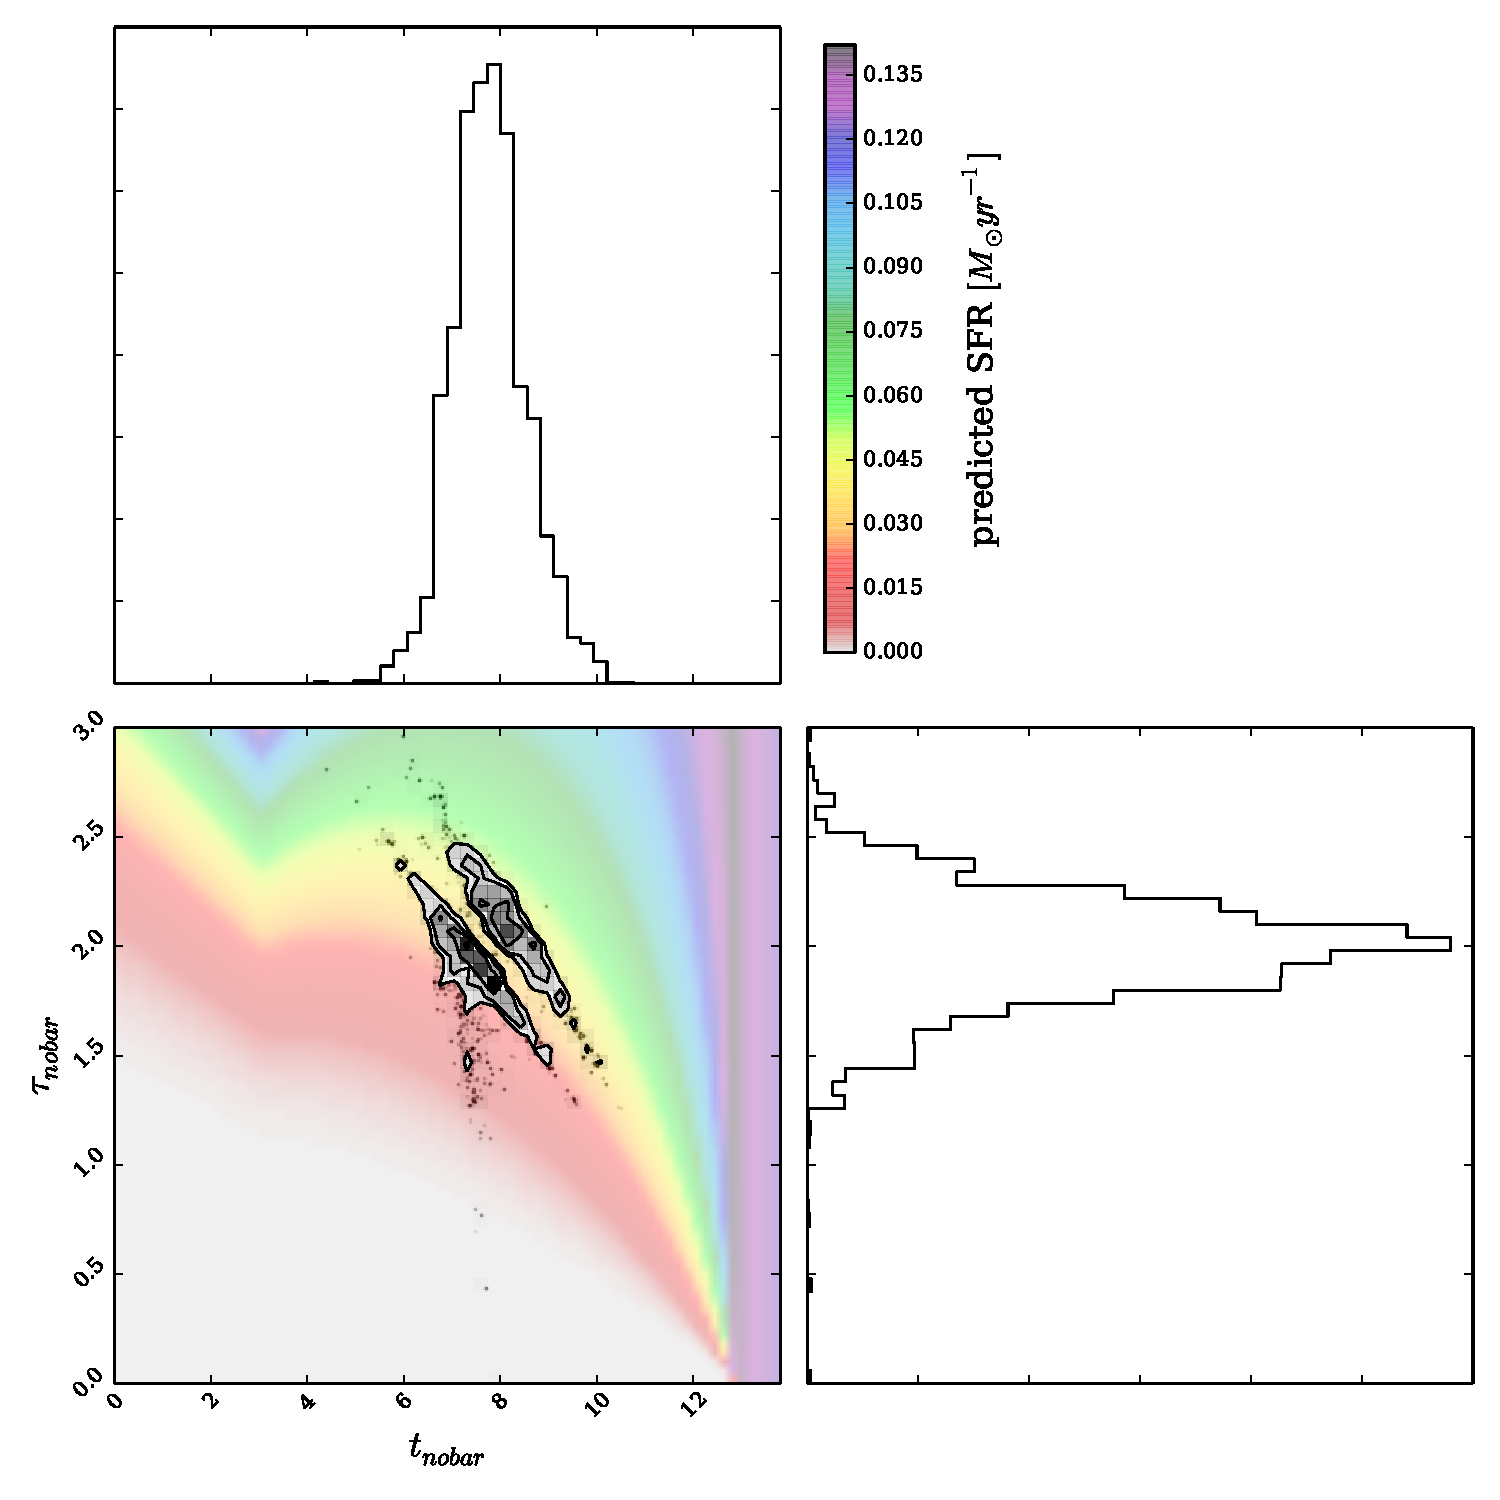
\includegraphics[width=0.4975\textwidth]{no_bars.pdf}
%\caption{Same as for Figure \ref{all} but for barred and non barred galaxies.}
%\label{bars}
%\end{figure*}

In figure \ref{red_s} we can see those galaxies which are defined to be in the optical red sequence, show a prevalence for medium quenching timescales ($\tau \sim1.5~Gyr$) at early times for the smooth-like galaxies and slow quenching timescales ($\tau > 1.5~Gyr$) at medium for the disc-like galaxies; again confirming the results found by \citet{Sch2014}. We can see that the areas of high likelihood for the disc-like galaxies occupy areas that also have some residual star formation occurring after evolving with very slow quenching timescales, suggesting that the disc galaxies which make up the red sequence seem to reside at its edge, on the border with the green valley. 

For the smooth parameters in the left panel of figure \ref{red_s} we also get some high likelihood for slow quenching timescales ($\tau > 1.5~Gyr$) at very early times, which according to figure \ref{all} should not be the case. Perhaps this is the influence of intermediate galaxies (with $p_s \sim p_d \sim 0.5$), hence why similar high likelihood areas exist for both the smooth-like and disc-like galaxies. Considering there are far more of these intermediate galaxies than those that are definitively early-types (see table \ref{subs}) these galaxies have overwhelmed the likelihoods creating a bimodality in the likelihoods. This is also the case for the disc-like galaxies suggesting that there is still a morphological bimodality in both populations.

In figure \ref{red_s_clean} we try to remove the influence from these intermediate galaxies; the figure shows the SFH parameters but only for those galaxies defined to be both in the optical red sequence and the GZ2 `clean' samples (i.e. $p_d \geq 0.8$ and $p_s \geq 0.8$). This enables us to disentangle which galaxies are contributing to which areas of high likelihood in figure \ref{red_s}. We can therefore see that the typical clean, smooth, red sequence galaxy has undergone a SFH with a relatively rapid quench at various early times, resulting in a very low current SFR. These are therefore the typical \emph{`red and dead'} galaxies expected to be found in the red sequence. Note however that still, there is only a small amount of likelihood for quenching timescales below ($\tau < 1.0~Gyr$) and that the early-type galaxies favour a medium quenching. 

What has disappeared from the parameter likelihood space is the preference for slow quenching at very early times, this suggests that it is the intermediate galaxies with $0.5 < p_s < 0.8$ which were contributing to this region of likelihood. These galaxies are those whose morphology cannot easily be distinguished or deliberated either because it is at a large distance or because it is an S0 galaxy whose morphology can be deliberated by different users in different ways. These galaxies were behaving more like disc galaxies than smooth ones. 

%However for the clean disc  galaxies in the red sequence (presumably the red spiral galaxies, ?) there is no region of the parameter space which has a preferred higher likelihood, suggesting that although these disc galaxies are optically red, they have a wide range of NUV-u colours, giving rise to a wide range of timescales for the most recent episode of star formation. Although we can pick out a similar region of high likelihood, for fast quenching at early times for disc galaxies as seen for smooth galaxies in the left panel of figure \ref{red_s_clean}, we can see a preference for high likelihood across all regions of the parameter space. This suggests that there is no `typical' red sequence disc galaxy and that there are many possible routes for a disc galaxy to the red sequence. 

We can also see the influence from removing the intermediate galaxies on the likelihoods for the disc parameters; we no longer have a bimodal distribution, instead one that clearly favours very slow quenching at relatively early times. However we do still have a tail towards a preference for more rapid quenching at more recent times, however none with $\tau < 1.0~Gyr$ suggesting that disc galaxies do not make it to the red sequence via this rapid mechanism.

This preference for large quenching timescales suggests that these galaxies have only just reached the red sequence after a very slow evolution across the colour-magnitude diagram. Considering their limited number it is likely that these galaxies are currently on the edge of the red sequence having recently (and finally) moved off the green valley.

This has many implications for green valley galaxies, as all of these routes must have passed through this region on their way to the red sequence. We therefore expect to see a similar distribution of likelihoods for the green valley disc-like and smooth-like galaxies but perhaps at later quenching times, pre-empting what will become the red sequence over time. 

\subsection{Green Valley Galaxies}


In figures \ref{gv} and \ref{gv_clean} we can make similar comparisons for the green valley galaxies as we did previously for the red sequence. In figure \ref{gv} we still see the correlation between the two parameters as seen in figure \ref{all} but the areas of high likelihood for the parameters have changed. We no longer have a trimodal likelihood in the parameter space for smooth galaxies but retain a bimodal likelihood for the parameters for the disc-like green valley galaxies. 

We can also see that quenching for the green valley occurs on similar quenching timescales to that of the red sequence; there is little to no likelihood for $\tau$ below $\sim 1.0 ~Gyr$ for either the smooth- or disc-like galaxies, unlike in the previous plots, however at differing quenching times. We also see for the disc-like galaxies a preference for very slow quenching at recent times which we believe to be those galaxies that have only just left the edge of the blue cloud and entered the green valley, hence they have some higher recent star formation than the other galaxies in the blue cloud.

There is a very little likelihood however, for rapid quenching of the smooth-like galaxies. This may be counter intuitive at first, as one of the main arguments for the lack of galaxies in the green valley is due to the hypothesised rapid movement across it; however, if this is the case then catching a galaxy with this quenching history will be difficult. Especially considering the amount of intermediate galaxies which are present in the green valley compared to those that are in the clean samples. These galaxies will be overwhelming the `walker' positions in the algorithm. 

Therefore if we remove the influence of such galaxies as in figure \ref{gv_clean}, which shows the regions of high likelihood for the model parameters for only the `clean' green valley galaxies, we can see that we do indeed detect some very rapid quenching at very recent times. However we only find this for smooth galaxies, just as in figure \ref{red_s_clean} suggesting again that it is only early-type galaxies which can progress through the green valley and into the red sequence in such a way. 

For the disc-like galaxies, whose parameters were also overwhelmed by the sheer number of intermediate galaxies in the green valley, we can see a large shift in likelihood for the clean disc galaxies seen in the right panel of figure \ref{gv_clean}. Upon removal of the intermediate galaxies the regions of high likelihood now reside at much longer quenching timescales, as expected for a late-type galaxy.  We still retain some likelihood for galaxies with higher SFR than the other galaxies, suggesting there are also some late-type galaxies that have just progressed from the blue cloud into the green valley. 

Given enough time, these galaxies will eventually pass fully through the green valley and make it out to the other side in the red sequence (the right panel of figure \ref{sfr_mass_col} shows galaxies with $\tau > 1.0~Gyr$ do not approach the red sequence within $3~Gyr$ post quench). This is most likely the origin of the `red spirals' and explains why there are currently so few of them. If our Universe was older this suggests we would observe more red spirals on the red sequence. 

We can see by comparing figure \ref{gv_clean} with figure \ref{red_s_clean} for the clean red sequence galaxies, that both populations the parameters occupy similar regions of space in the $\tau$ parameter but have gained a shift to later times in the $t$ parameter. This means that both populations are tracing the evolution of the red sequence confirming that green valley is indeed a transitional population between blue cloud and red sequence regardless of morphology. Currently as we observe the green valley, it's main constituent are very slowly evolving disc-like galaxies along with intermediate- and some smooth-like galaxies which manage to pass across it within $\sim 1.0-1.5~Gyr$.

All of this evidence suggests that there are not just two routes for galaxies through the green valley but \emph{three}: with the smooth- ($1.0 < \tau < 1.5 ~Gyr$), intermediate- ($1.5 < \tau < 2.0~Gyr$) and disc-like ($\tau > 2.0~Gyr$) galaxies each having different SFHs which lead them across the green valley, given enough cosmic time. In this instance, the grass is always redder on the other side.


\subsection{Blue Cloud Galaxies}
Since the blue cloud is considered to be primarily made of star forming galaxies we expect the model to have some difficulty in determining the most likely quenching model to describe them, considering . In figure \ref{blue_c} both sets of parameters show high likelihood for slow quenching at late times, with a higher likelihood for the disc-like galaxies. We believe that this is the model picking up on those galaxies which have so far not undergone any quenching. However we also see a trimodality in both sets of parameters, again which is more pronounced in the disc-like galaxies, suggesting that there is still quenching occurring within the blue cloud. We note that in this case there is no quenching below $\tau \sim 1.0~Gyr$ for either population, confirming that any galaxy undergoing a rapid quench will very quickly leave the blue cloud. 

There is also high likelihood in both samples for medium rate quenching at relatively recent times which could account for those galaxies near the edge of the blue cloud that have begun to quench. This area of high likelihood is again at very similar ranges of the quenching timescale $\tau$, but occurring at yet earlier quenching times, $t_q$, suggesting that those galaxies which have begun to quench in the blue cloud are already tracing the parameters of the green valley. Confirming once more that the green valley is a transitional population between the blue cloud and red sequence regardless of morphology.

The SFH parameter space for the smooth-like and disc-like galaxies appear very similar, suggesting so too are galaxies in the blue cloud, irrespective of their morphology. Of all of the regions of the CMD, this is to be expected in the blue cloud since it consists of galaxies that are mostly still star forming. The way these galaxies differ is the mechanisms and triggers by which they have formed their stars, having no effect on the observed colours but a discernible effect on their morphologies.

When we compare figures \ref{blue_c} and \ref{blue_c_clean} which shows the likely model parameters for the `clean' blue cloud galaxies, only the smooth galaxies have high likelihood for a slow quench model at late times, suggesting that most of the obviously smooth blue galaxies in the GZ2 sample still have star formation occurring. 

The disc-like galaxies in the right panel of figure \ref{blue_c_clean} show a high likelihood for any timescale of quenching at late times, which again is most likely indicative of star formation still occurring. We still retain some preference however for medium quenching at recent (late) times (which we do not for the smooth parameters), suggesting that the edge of the blue cloud is made primarily of disc-like galaxies rather than the smooth-like galaxies, as is observed.


\section{Discussion}\label{diss}
%Build up of red sequence - many paths passed through the green valley previously.
%\\ Green valley both static and transitional
%\\ Spare because fraction of galaxies quenching at any one time is few
%\\ Different paths across for smooth, intermediate and disc galaxies
%\\ Methods for quenching - Binney + fountain models cut off when galaxy starts to move through IGM. 
The results from the previous section allow us to build up a picture of a galaxy's journey from the blue cloud to the red sequence as it evolves. Firstly, there is a definitive morphological dependance on the evolution of a galaxy; smooth- and disc-like galaxies evolve with very different quenching timescales, but what is the mechanism driving this difference? We can put constraints on this by considering how they evolve differently.

We can confirm that the green valley is indeed a transitional population for all morphologies, with many different SFH parameters to describe the possible path of a galaxy through it, as shown by the parameters for the green valley galaxies tracing those of the red sequence but at earlier quenching times. The only morphological difference is for the rate at which galaxies transition through it; only smooth-like galaxies pass through rapidly, whereas disc-like galaxies pass through much more slowly. We therefore theorise that with enough cosmic time, eventually late-type galaxies will come to populate the red sequence as well as early-types. At our current epoch and at the timescales at which disc-like galaxies are found to be quenching we therefore would not see a large number of red disc-like galaxies, which is supported by our observations of the frequency of `red-spiral' galaxies \citep{Bamford09, Skibba09, Masters10, Masters10b}.

Therefore the green valley consists of a composite transiting population of disc-like galaxies which pass very slowly though (with only a small number having it made it to the red sequence at the current time) and smooth-like galaxies which pass through so rapidly we have very minimal likelihood for rapid quenching. We also argue that there is a third population residing in the green valley from the intermediate galaxies (by comparing figures \ref{gv} and \ref{gv_clean}) which are passing through at middling quenching timescales. Since \citet{Sch2014} did not consider intermediate galaxies, their conclusions that there are 2 routes through the green valley for galaxies contradicts with our statements that their are currently three routes, dependant on whether a galaxy is early-, intermediate- or late-type. 

Clean blue cloud early-type galaxies have high likelihoods clustered only at late times with slow quenching timescales suggesting that these galaxies have not undergone any quenching and cannot be described by our quenching model. This confirms the theories concerning blue early-type galaxies \citep{Sch09} as previously `red and dead' ellipticals that have had recently promoted new star formation.

Another important point to discuss is the lack of likelihood for rapid quenching timescales $\tau < 1.0~Gyr$. This is most apparent in the disc parameters where no likelihood below this is detected, except at very recent times for the clean disc blue cloud galaxies. For the smooth galaxies only a small amount of likelihood is found for these extremely rapid quenching timescales, this suggests the mechanism which drives this quenching is only apparent for smooth-like galaxies and not for disc-like galaxies and is also extremely rare. We believe that this coincides with what we know about major mergers. 

Major mergers, once thought to be the main drivers of galactic evolution \citep{WR78, KWG93, LC93, DeL06, BLB08} are now believed to be much rarer events \citep{Darg, Hopkins12, Brook12}. They are also considered to be very violent events causing huge bursts of star formation which rapidly use all of the available cold gas for star formation, triggering AGN activity which in turn is thought to quench star formation \citep{Sch10, Sanders88, Hopkins06, Sch2014} and trigger a major morphological transformation to an early-type galaxy \citep{BH96, Darg}. Hence, we do not detect likelihood at rapid quenching for disc galaxies because all of those which have undergone a quench such as this (for example our own galaxy when it collides with M31 in $2~Gyrs$ time) have become smooth in morphology. We then find a scattering of likelihood (due to the rarity of major mergers) at these rapid quenching timescales for the smooth-like galaxies; the remnants of these major mergers. 

There is also a strong preference at all quenching times for the intermediate galaxies to have middle quenching timescales ($\tau \sim 1.5~Gyr$). Minor mergers, which are thought to promote star formation in a similar but not as drastically as major mergers \citep{Darg, Kav09}, are thought to also trigger AGN activity \citep{Sch10, Sch2014} which can cause a quenching of star formation but at a slower rate than a major merger. Such minor mergers can cause some morphological changes to a featured galaxy but do not completely destroy the disc \citep{Darg}. In figure 6 of \citet{Darg} we can see that minor mergers with mass ratio's over 1:100 are typically spiral-spiral interactions and also display typically green optical colours; the merger remnants would be classified as green valley. We therefore believe that a minor merger can cause both a quench on a medium timescale along with a morphological change from a spiral to an intermediate galaxy.

However minor mergers are also as rare as major mergers. Therefore any trigger of AGN activity could also have the same effect, along with galaxy harassment, interactions, ram pressure stripping and cluster interactions; any mechanism that can cause a depletion in the cold gas available without disturbing the disc structure within a galaxy would fall into the \emph{medium quenching} category. These along with major mergers can be considered as external quenching processes. Considering the majority of galaxies reside in clusters it is not surprising that the majority of our galaxies are considered to be intermediate in morphology. 

For the clean disc galaxies across all of the populations the highest likelihood always occurs at the largest quenching timescales. This means for those disc galaxies whose morphology is least contested, i.e. most obviously spiral or barred, they evolve across the colour-magnitude diagram with cosmic time extremely slowly. Such a SFH does not deplete a galaxy of it's cold gas supply entirely but merely reduces the amount of star formation occurring over time without anything untoward occurring to upset this gentle decline. This suggests that the preference for late-type galaxies moving across the colour-magnitude diagram is via evolution that is secular in nature (i.e. non-violent mechanisms often occurring in isolated environments which are internal to the galaxy, \citealt{KK04, Sheth12}). This can include the shut down of feedback of cold gas from the galactic halo or IGM (Binney's stuff) or through the formation of a bar, which are thought to channel gas towards the centre of a galaxy \citep{Masters10, Cheung13, Melvin14}.


\section{Conclusion}\label{conc}
We have used morphological classifications from the Galaxy Zoo 2 project to determine the morphological dependant star formation histories of galaxies through a Bayesian analysis of an exponentially declining star formation rate model of quenching. We determined the most likely parameters for the quenching time, $t_q$ and quenching timescale $\tau$ in this model for galaxies across the blue cloud, green valley and red sequence to trace galactic evolution across the colour-magnitude diagram. We find that the green valley is indeed a transitional population for all morphological types, however this transition proceeds much slower for disc-like galaxies and can occur very rapidly for smooth-like galaxies. We conclude that:
\begin{enumerate}
\item There is a clear correlation between $t_{quench}$ and $\tau$. At earlier times, the quenching timescale is longer, whereas at more recent times, the quenching timescale is shorter on average suggesting an environmental quenching dependance with cosmic time
\item The most likely SFH parameters for the green valley trace those for the red sequence at later times, pre-empting the formation of the red sequence suggesting that the green valley is indeed a transitional population with morphological dependant routes through it
\item There are three possible routes through the green valley dependant on morphology for smooth-like, intermediate and disc-like galaxies. These are thought to be caused by major mergers, minor mergers/galaxy interactions/AGN activity and secular evolution respectively.
\end{enumerate}

There is not one specific route to each part of the colour-colour or colour-magnitude diagram, due to the complex interplay between the SFH parameters, however the morphology of a galaxy reveal the previous possible steps to reach it's current location. If a galaxy is a late-type at the current epoch, independent of where it is on the colour-magnitude diagram) then it cannot have undergone rapid quenching and consequently any mechanism that drives this, such as a major merger. Conversely for a galaxy to be early-type at the current epoch, independent of where it is on the colour-magnitude diagram then it cannot have undergone slow quenching and consequently any mechanism that drives this, such as secular evolution. 

\section*{Acknowledgements}
The authors would like to thank D. Forman-Mackey and P. Marshal for extremely useful Bayesian statistics discussions and J. Binney for an interesting discussion on the nature of quenching and feedback in disc galaxies. GALEX would like to thank NASA. SDSS would like to thank lots of people. This publication made extensive use of the Tool for Operations on Catalogues And Tables (TOPCAT) which can be found at \url{http://starlink.ac.uk/topcat/}. This research has also made use of NASA's ADS service and Cornell's ArXiv. 

\begin{thebibliography}{}
\bibitem[\protect\citeauthoryear{Aihara et al.}{2011}]{Aihara11} Aihara, H. et al., 2011, ApJSS, 193, 29
\bibitem[\protect\citeauthoryear{Arnouts et al.}{2007}]{Arnouts07} Arnouts, S. et al., 2007, A\&A, 476, 137
\bibitem[\protect\citeauthoryear{Baldry et al.}{2004}]{Baldry04} Baldry, I. K. et al., 2004, ApJ, 600, 681
\bibitem[\protect\citeauthoryear{Baldry et al.}{2006}]{Baldry06} Baldry, I. K. et al., 2006, MNRAS, 373, 469
\bibitem[\protect\citeauthoryear{Ball, Loveday \& Brunner}{2008}]{BLB08} Ball, N. M., Loveday, J. \& Brunner, R. J., 2008, MNRAS, 383, 907
\bibitem[\protect\citeauthoryear{Bamford et al.}{2009}]{Bamford09} Bamford, S. P. et al., 2009, MNRAS, 393, 1324
\bibitem[\protect\citeauthoryear{Barnes \& Hernquist}{1996}]{BH96} Barnes, J. E. \& Hernquist, L., 1996, ApJ, 471, 115
\bibitem[\protect\citeauthoryear{Bell et al.}{2004}]{Bell04} Bell, E. F. et al., 2004, ApJ, 608, 752
\bibitem[\protect\citeauthoryear{B\'ethermin et al.}{2012}]{Beth} B\'ethermin, M. et al., 2012, ApJ, 757, L23
\bibitem[\protect\citeauthoryear{Blanton et al.}{2005}]{Blanton05} Blanton, M. R. et al., 2005, AJ, 129, 2562
\bibitem[\protect\citeauthoryear{Blanton \& Roweis}{2007}]{BR07} Blanton, M. R. \& Roweis, S., 2007, AJ, 133, 734
\bibitem[\protect\citeauthoryear{Brammer et al.}{2009}]{Brammer09} Brammer, G. B. et al., 2009, ApJ, 706, 173
\bibitem[\protect\citeauthoryear{Brinchmann et al.}{2004}]{Brinch04} Brinchmann, J. et al., 2004, MNRAS, 351, 1151
\bibitem[\protect\citeauthoryear{Brook et al.}{2012}]{Brook12} Brook, C. B. et al., 2012, MNRAS, 419, 771
\bibitem[\protect\citeauthoryear{Bruzual \& Charlot}{2003}]{BC03} Bruzual, G. \& Charlot, S., 2003, MNRAS, 344, 1000
\bibitem[\protect\citeauthoryear{Cardelliet et al.}{1989}]{Cardelli89} Cardelli, J. A. et al., 1989, ApJ, 345, 245
\bibitem[\protect\citeauthoryear{Chen et al.}{2010}]{Chen10} Chen, X. Y. et al., 2010, A\&A, 515, 101
\bibitem[\protect\citeauthoryear{Cheung et al.}{2013}]{Cheung13} Cheung, E. et al., 2013, ApJ, 779, 162
\bibitem[\protect\citeauthoryear{Conroy, Gunn \& White}{2009}]{CGW09} Conroy, C., Gunn, J. E. \& White, M. 2009, ApJ, 699, 486
\bibitem[\protect\citeauthoryear{Darg et al.}{2009}]{Darg} Darg, D. et al., 2009, MNRAS, 401, 1552
\bibitem[\protect\citeauthoryear{DeLucia et al.}{2006}]{DeL06} DeLucia, G. et al., 2006, MNRAS, 366, 499
\bibitem[\protect\citeauthoryear{Elbaz et al.}{2011}]{Elbaz11} Elbaz, D. et al., 2011, A\&A, 533, A119
\bibitem[\protect\citeauthoryear{Eminian et al.}{2008}]{Eminian08} Eminian, C. et al., 2008, MNRAS, 384, 930
\bibitem[\protect\citeauthoryear{Faber et al.}{2007}]{Faber07} Faber, S. M. et al., 2007, ApJ, 665, 265
\bibitem[\protect\citeauthoryear{Falkenberg et al.}{2009}]{Falk09} Falkenberg, M. A. et al., 2009, MNRAS, 397, 1954
\bibitem[\protect\citeauthoryear{Foreman-Mackey et al.}{2013}]{Dan} Foreman-Mackey, D., Hogg, D. W., Lang, D., Goodman, J., 2013, PASP, 125, 306
\bibitem[\protect\citeauthoryear{Goodman \& Weare}{2010}]{GW10} Goodman, J. \& Weare, J., 2010, CAMCS, 5, 65
\bibitem[\protect\citeauthoryear{Gon\c calves et al.}{2012}]{Gonc12} Gon\c calves, T. S. et al., 2012, ApJ, 759, 67
\bibitem[\protect\citeauthoryear{Gonz\'alez et al.}{2010}]{Gonzalez} Gonz\'alez, V. et al., 2010, ApJ, 713, 115
\bibitem[\protect\citeauthoryear{Heinis et al.}{2014}]{Heinis14} Heinis, S. et al., 2014, MNRAS, 437, 1268
\bibitem[\protect\citeauthoryear{Hopkins et al.}{2006}]{Hopkins06} Hopkins, P. F. et al., 2006, ApJS, 163, 1
\bibitem[\protect\citeauthoryear{Hopkins et al.}{2012}]{Hopkins12} Hopkins, P. F. et al., 2012, MNRAS, 427, 968
\bibitem[\protect\citeauthoryear{Jarosik et al.}{2011}]{WMAP} Jarosik, N. et al., 2011, ApJSS, 192, 18
\bibitem[\protect\citeauthoryear{Kauffman, White \& Guiderdoni}{1993}]{KWG93} Kauffman, G., White, S. D. M. \& Guiderdoni, B., 1993, MNRAS, 264, 201
\bibitem[\protect\citeauthoryear{Kauffmann et al.}{2003}]{Kauff03} Kauffman, G. et al., 2003, MNRAS, 341, 33
\bibitem[\protect\citeauthoryear{Kaviraj et al.}{2009}]{Kav09} Kaviraj, S. et al. 2009, MNRAS, 394, 1713
\bibitem[\protect\citeauthoryear{Kormendy \& Kennicutt}{2004}]{KK04} Kormendy, J. \& Kennicutt, R. J., 2004, ARA\&A, 42, 603
\bibitem[\protect\citeauthoryear{Kreik et al.}{2010}]{Kreik10} Kreik, M. et al., 2010, ApJL, 722, L64
\bibitem[\protect\citeauthoryear{Lacey \& Cole}{1993}]{LC93} Lacey, C. \& Cole, S., 1993, MNRAS, 262, 627
\bibitem[\protect\citeauthoryear{Lee et al.}{2012}]{Lee12} Lee, K.-S. et al., 2012, ApJ, 752, 66
\bibitem[\protect\citeauthoryear{Lintott et al.}{2009}]{Lintott09} Lintott, C. J. et al., 2009, MNRAS, 399, 129
\bibitem[\protect\citeauthoryear{Lintott et al.}{2011}]{Lintott11} Lintott, C. J. et al., 2011, MNRAS, 410, 166
\bibitem[\protect\citeauthoryear{MacKay}{2003}]{MacKay} MacKay, D. J. C., 2003, \emph{Information Theory, Inference and Learning Algorithms}, Cambridge University Press, ISBN 978-0-521-64298-9
\bibitem[\protect\citeauthoryear{Marasco, Fraternali \& Binney}{2012}]{MFB12} Marasco, A., Fraternali, F. \& Binney, J. J., 2012, MNRAS, 419, 1107
\bibitem[\protect\citeauthoryear{Maraston et al.}{2006}]{Maraston06} Maraston, C. et al., 2006, MNRAS, 362, 799
\bibitem[\protect\citeauthoryear{Martin et al.}{2005}]{Martin05} Martin, D. C. et al., 2005, ApJ, 619, L1
\bibitem[\protect\citeauthoryear{Martin et al.}{2007}]{Martin07} Martin, D. C. et al., 2007, ApJS, 173, 342
\bibitem[\protect\citeauthoryear{Masters et al.}{2010a}]{Masters10} Masters, K. L. et al., 2010, MNRAS, 405, 783
\bibitem[\protect\citeauthoryear{Masters et al.}{2010b}]{Masters10b} Masters, K. L. et al., 2010, MNRAS, 404, 792
\bibitem[\protect\citeauthoryear{Masters et al.}{2011}]{Masters11} Masters, K. L. et al., 2011, MNRAS, 411, 2026
\bibitem[\protect\citeauthoryear{Masters et al.}{2012}]{Masters12} Masters, K. L. et al., 2012, MNRAS, 424, 2180
\bibitem[\protect\citeauthoryear{Melbourne et al.}{2012}]{Mel12} Melbourne, J. et al., 2012, ApJ, 748, 47
\bibitem[\protect\citeauthoryear{Melvin et al.}{2014}]{Melvin14} Melvin, T et al., 2014, MNRAS, 438, 2882
\bibitem[\protect\citeauthoryear{Mendez et al.}{2011}]{Mendez11} Mendez, A. J. et al., 2011, ApJ, 736, 110
\bibitem[\protect\citeauthoryear{Miller, Rose \& Cecil}{2011}]{MRC11} Miller, N. A., Rose, J. A. \& Cecil, G. 2011, ApJL, 727, L15
\bibitem[\protect\citeauthoryear{Noeske et al.}{2007}]{Noeske07} Noeske, K. G. et al., 2007, ApJ, 660, L43
\bibitem[\protect\citeauthoryear{Oh et al.}{2011}]{Oh11} Oh, K. et al., 2011, ApJS, 195, 13
\bibitem[\protect\citeauthoryear{Padmanabhan et al.}{2008}]{Pad08} Padmanabhan, N. et al., 2008, ApJ, 674, 1217
\bibitem[\protect\citeauthoryear{Peng et al.}{2010}]{Peng} Peng, Y. et al., 2010, ApJ, 721, 193
\bibitem[\protect\citeauthoryear{Robitaille et al.}{2013}]{Rob13} Robitaille, T. P. et al., 2013, A\&A, 558, A33
\bibitem[\protect\citeauthoryear{Salim et al.}{2007}]{Salim07} Salim, S. et al., 2007, ApJSS, 173, 267
\bibitem[\protect\citeauthoryear{Sanders et al.}{1988}]{Sanders88} Sanders, D. B. et al., 1988, ApJ, 325, 74
\bibitem[\protect\citeauthoryear{Schawinski et al.}{2007}]{Sch07} Schawinski, et al., 2007, MNRAS, 382, 1415
\bibitem[\protect\citeauthoryear{Schawinski et al.}{2009}]{Sch09} Schawinski, K. et al., 2009, MNRAS, 396, 818
\bibitem[\protect\citeauthoryear{Schawinski et al.}{2010}]{Sch10} Schawinski, K. et al., 2010, MNRAS, 711, 284
\bibitem[\protect\citeauthoryear{Schawinski et al.}{2014}]{Sch2014} Schawinski, K. et al., 2014 (arXiv: 1402.4814)
\bibitem[\protect\citeauthoryear{Schiminovich et al.}{2007}]{Schim07} Schiminovich, D. et al., 2007, ApJS, 173, 315
\bibitem[\protect\citeauthoryear{Sheth et al.}{2012}]{Sheth12} Sheth, K. et al., 2012, ApJ, 758, 136
\bibitem[\protect\citeauthoryear{Simmons et al.}{2013}]{Simmons13} Simmons, B. D. et al., 2013, MNRAS, 429, 2199
\bibitem[\protect\citeauthoryear{Sivia}{1996}]{Sivia} Sivia, D. S., 1996, \emph{Data Analysis: A Bayesian Tutorial}, Oxford University Press, ISBN 0-19-851889-7
\bibitem[\protect\citeauthoryear{Skibba et al.}{2009}]{Skibba09} Skibba, R. A. et al., 2009, MNRAS, 399, 966
\bibitem[\protect\citeauthoryear{Soklakov}{2002}]{Sok02} Soklakov, A. N., 2002, (arXiv:math-ph/0009007)
\bibitem[\protect\citeauthoryear{Taylor}{2005}]{Taylor05} Taylor, M. B., 2005, ASP Conference Series, 347
\bibitem[\protect\citeauthoryear{White \& Rees}{1978}]{WR78} White, S. D. M. \& Rees, M. J., 1978, MNRAS, 183, 341
\bibitem[\protect\citeauthoryear{Willett et al.}{2013}]{GZ2} Willett, K. et al., 2014, MNRAS, 435, 2835
\bibitem[\protect\citeauthoryear{Willmer et al.}{2006}]{Willmer06} Willmer, C. N. A. et al., 2006, ApJ, 647, 853
\bibitem[\protect\citeauthoryear{Wyder et al.}{2007}]{Wyder07} Wyder, T. K. et al., 2007, ApJS, 173, 293
\bibitem[\protect\citeauthoryear{York et al.}{2000}]{York00} York, D. G. et al., 2000, AJ, 120, 1579
\end{thebibliography}{}


\appendix
\section{The different SFHs of barred and non-barred galaxies}

\begin{figure*}
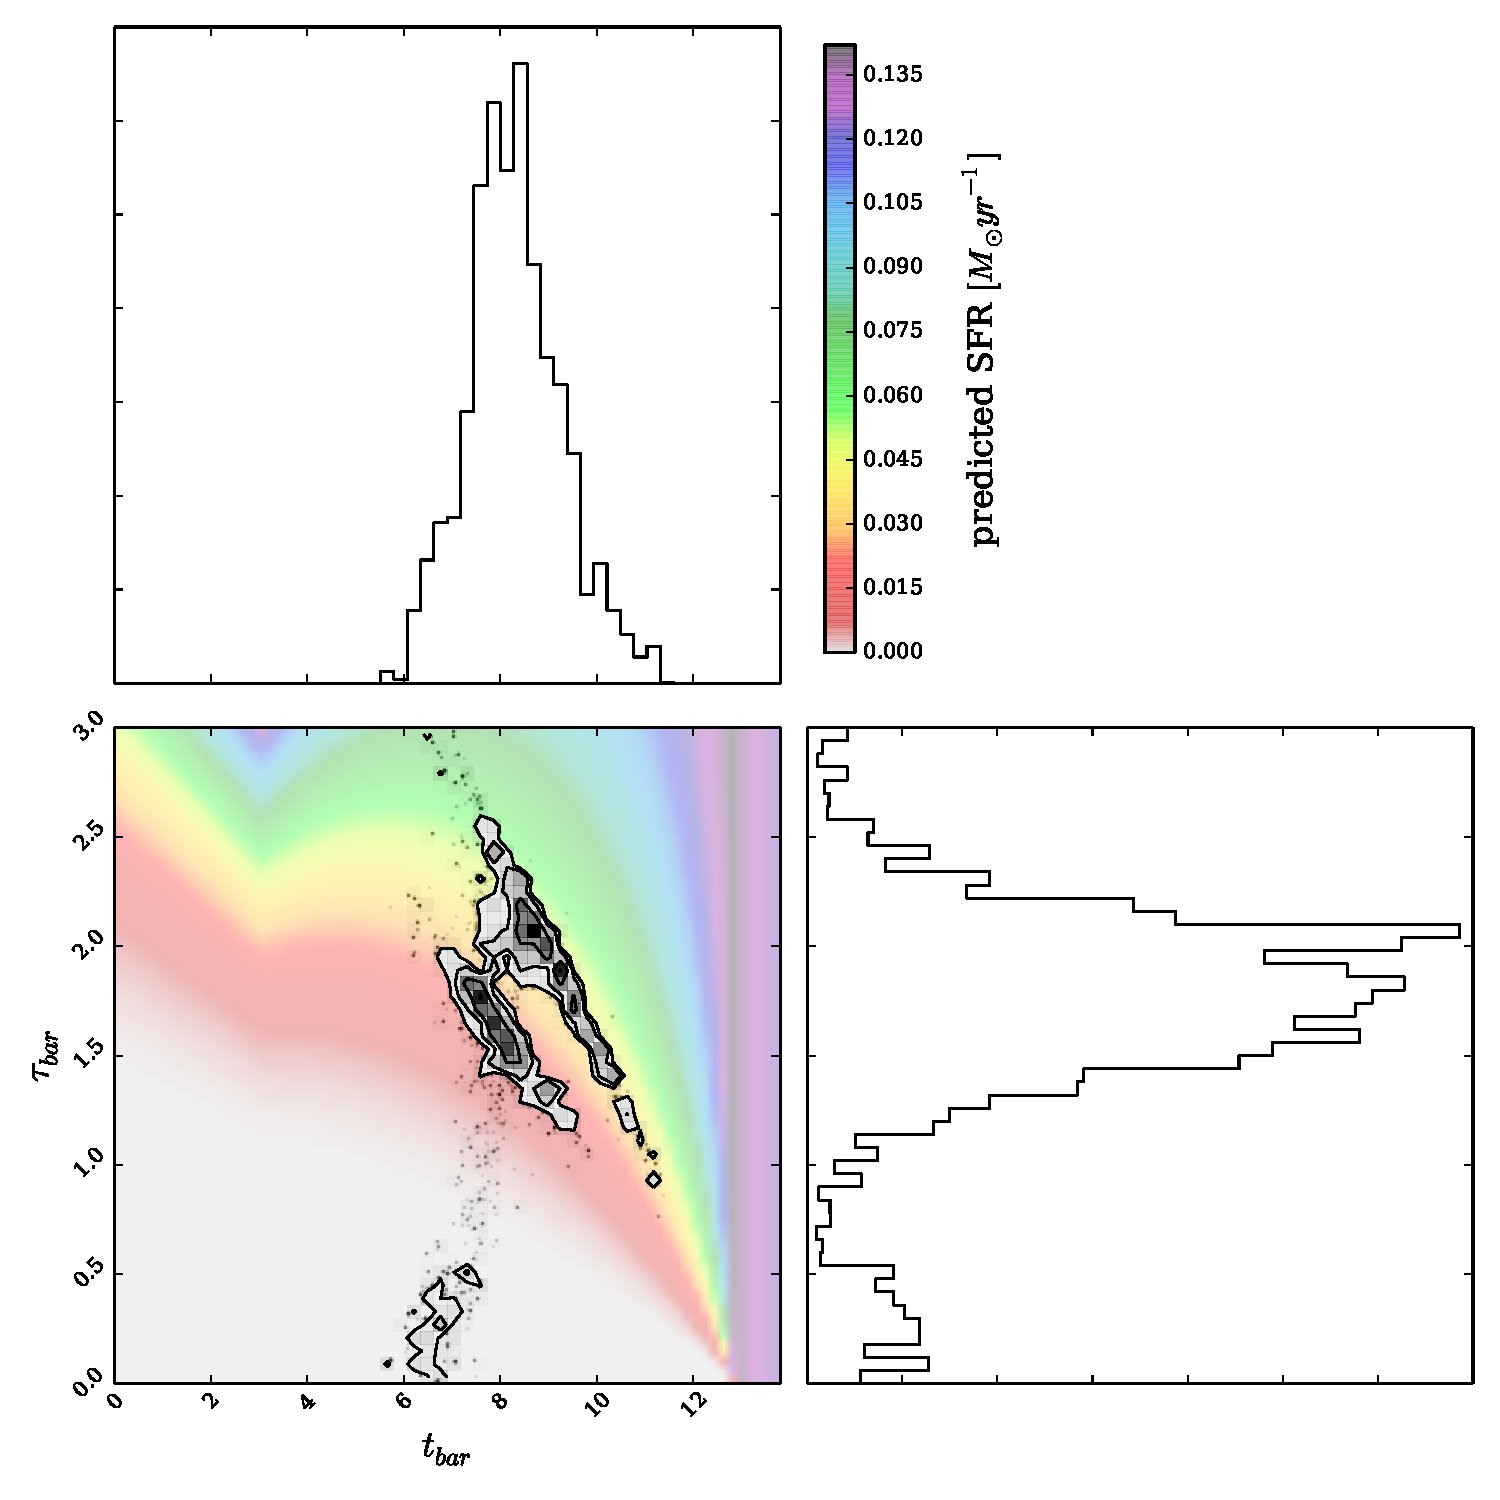
\includegraphics[width=0.4975\textwidth]{bars.pdf}
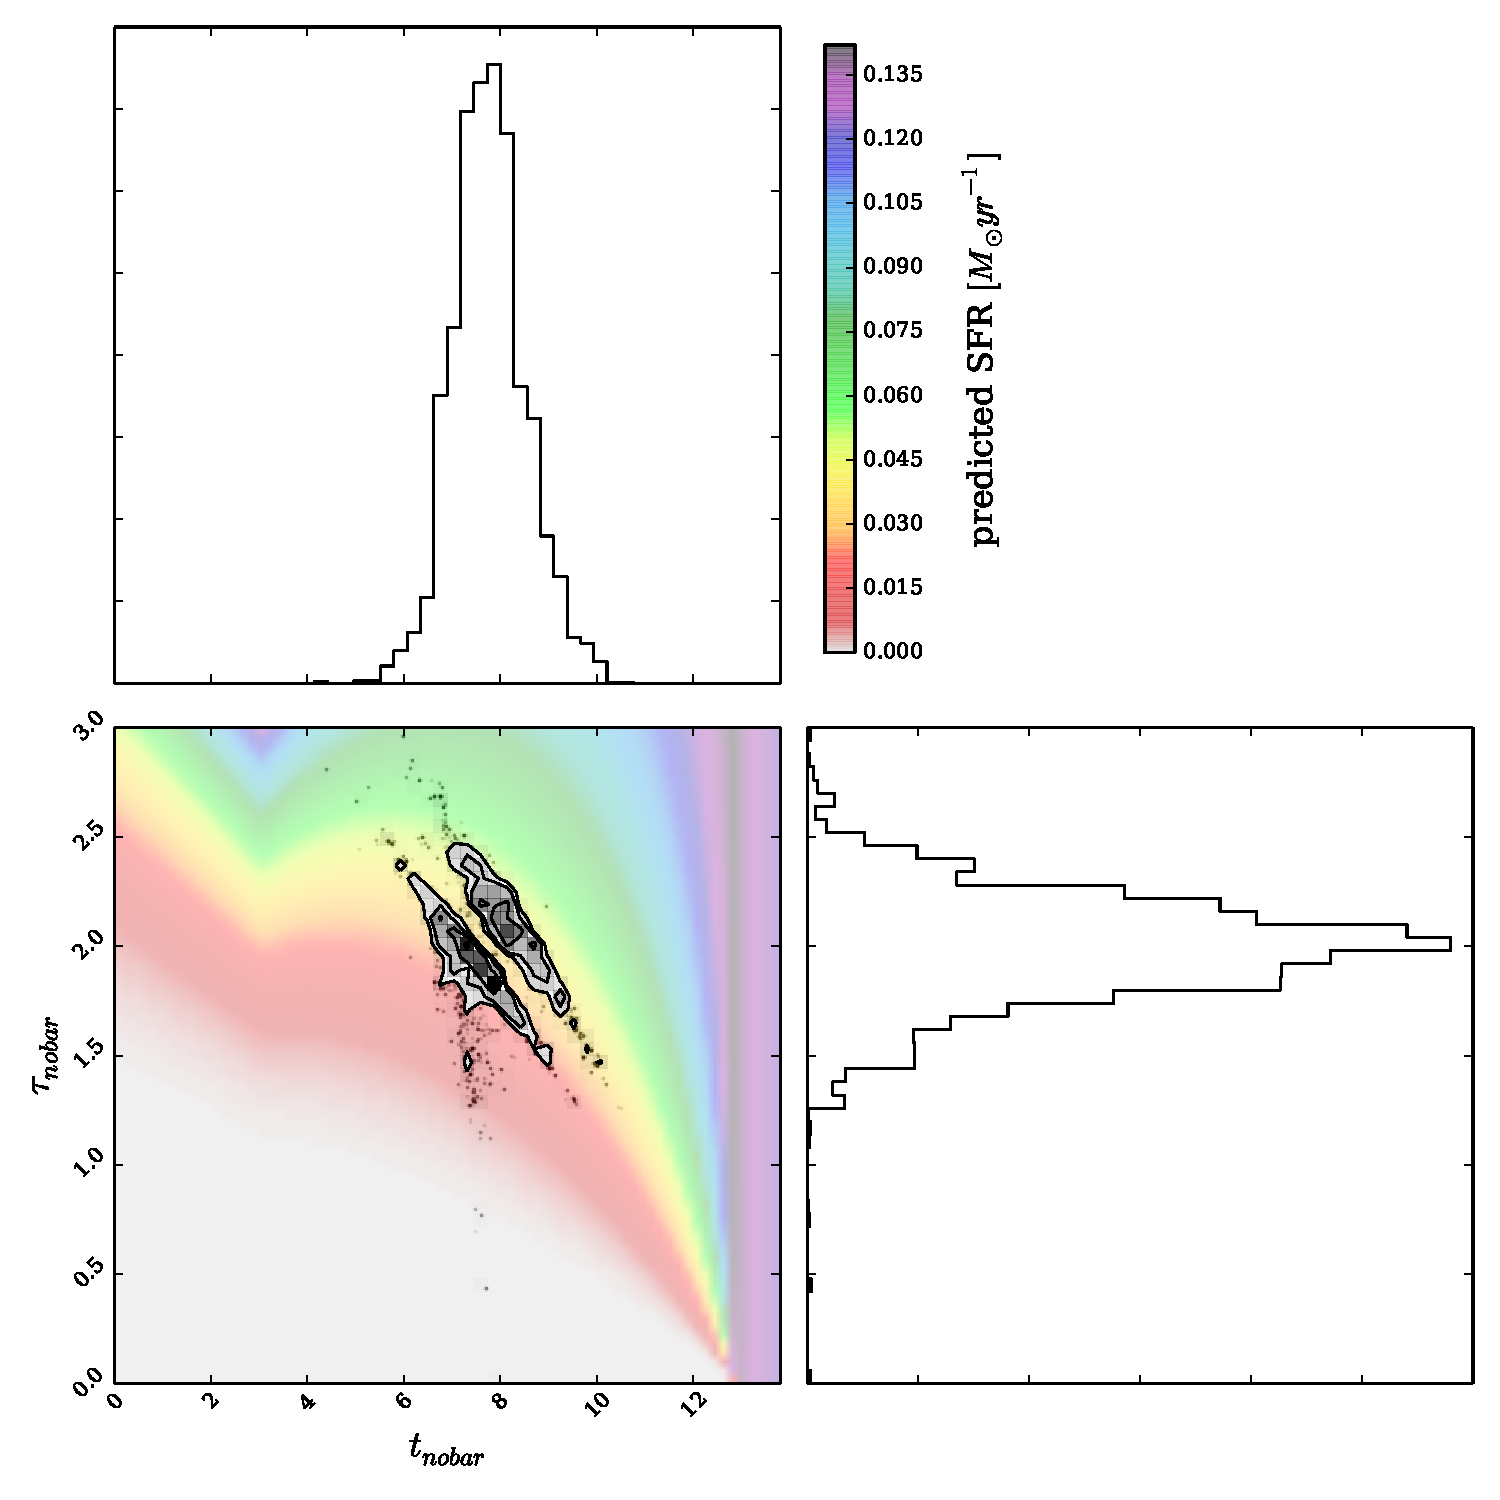
\includegraphics[width=0.4975\textwidth]{no_bars.pdf}
\caption{Same as for Figure \ref{all} but for barred and non barred galaxies.}
\label{bars}
\end{figure*}

In figure \ref{bars} we can compare the star formation history parameters for barred and unbarred galaxies, selected so that $N_{count, bar} > 10$ and $N_{count, no bar} > 10$. The analysis was then run with $p_{bar}$ and $p_{no bar}$ in place of $p_{smooth}$ and $p_{disc}$ in the final equation in section \ref{stats}. We can see that two the populations occupy different areas in the SFH parameter space suggesting that bars have indeed undergone a different formation history to non barred disc galaxies.  Barred galaxies simultaneously are more likely to have both bluer and redder colours than non barred galaxies, as the bimodality seen in the SFH parameters of the non barred galaxies in the right hand panel of figure \ref{bars} has moved apart. 

This suggests that the argument for whether bars promote or quench star formation rates in galaxies could have evidence for both possibilities. Perhaps the amount and distribution of gas present in a galaxy prior to the formation of the bar determines what effect the bar will have on the star formation rate. There is also a region of likelihood at very rapid quenching timescales for barred galaxies which is not present in the parameters for the non barred galaxies, supporting the hypothesis that bars turn galaxies red (\emph{cite Maraston papers here}). To explain what we see here we can say either that:
\begin{enumerate}
\item As a bar forms it can cause a rapid quenching of star formation in it's host galaxy,
\item A rapid quenching of star formation in a galaxy can cause a bar to form.
\end{enumerate}
This analysis however, does not allow for this to be determined. 

\section{Colour-colour diagram evolution}
\begin{figure*}
\centering{
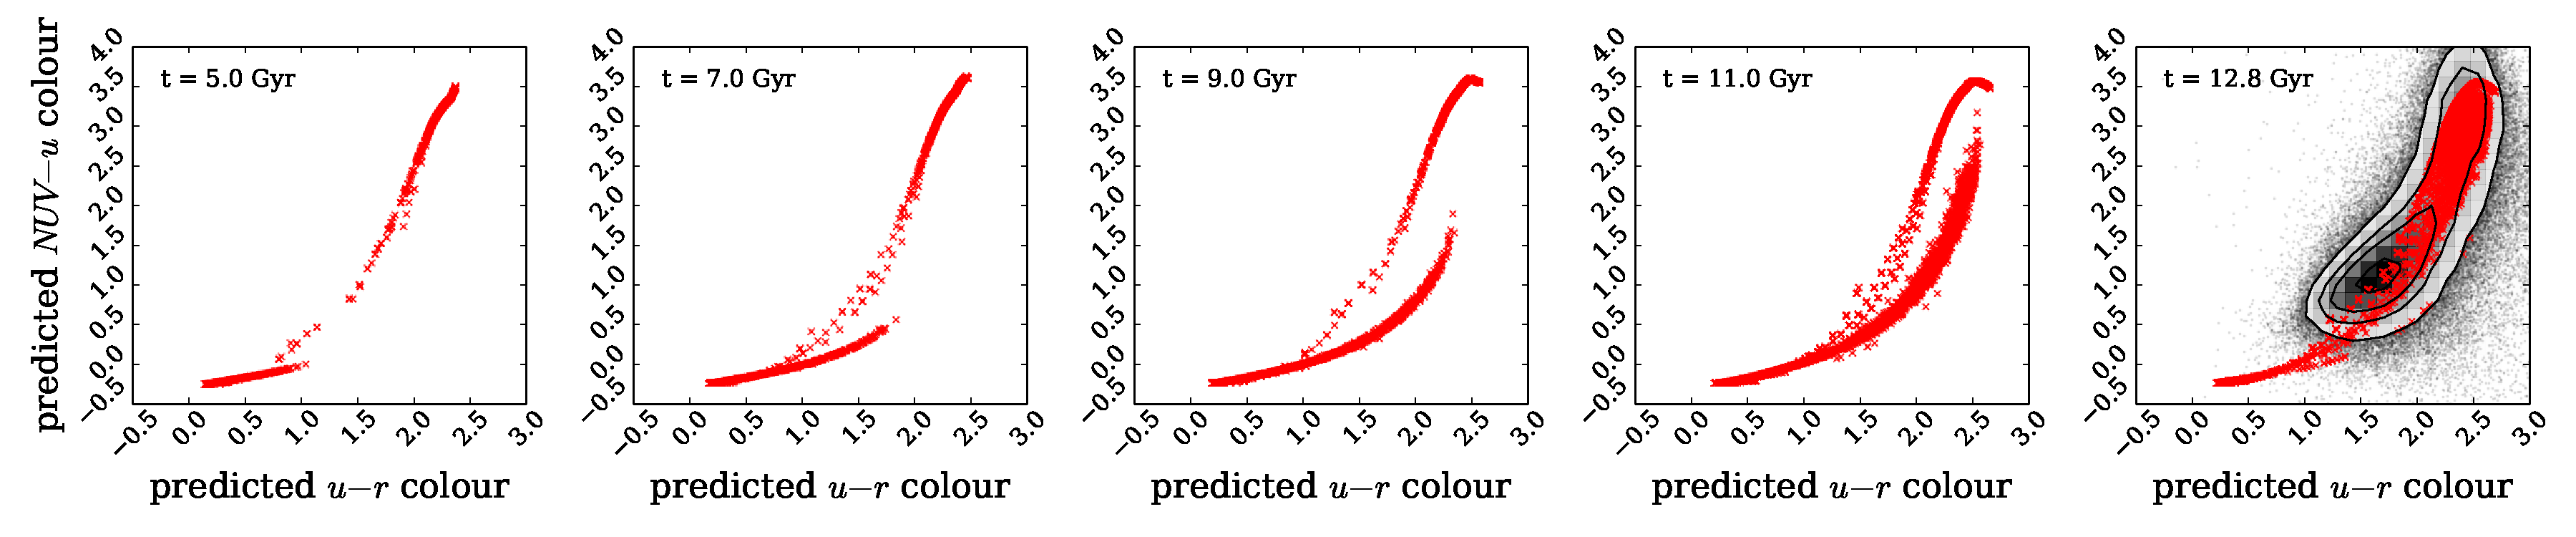
\includegraphics[width=\textwidth]{c_c_evo_numpy.pdf}}
\caption{Plots to show the evolution of the colour-colour diagram as predicted by the most likely exponential SFH model for each GZ2 galaxy. Each panel shows the model at different look-back times in the history of the Universe. The panel on the far right also includes the contours of the observed colours for the GZ2 galaxies in black, as well as the most likely predicted colours, in red, as a comparison.}
\label{c_c_evo}
\end{figure*}

\end{document}
